%==============================================================================
% Tento soubor použijte jako základ
% This file should be used as a base for the thesis
% Autoři / Authors: 2008 Michal Bidlo, 2022 Jaroslav Dytrych
% Kontakt pro dotazy a připomínky: sablona@fit.vutbr.cz
% Contact for questions and comments: sablona@fit.vutbr.cz
%==============================================================================
% kódování: UTF-8 (zmena prikazem iconv, recode nebo cstocs)
% encoding: UTF-8 (you can change it by command iconv, recode or cstocs)
%------------------------------------------------------------------------------
% zpracování / processing: make, make pdf, make clean
%==============================================================================
% Soubory, které je nutné upravit nebo smazat: / Files which have to be edited or deleted:
%   projekt-20-literatura-bibliography.bib - literatura / bibliography
%   projekt-01-kapitoly-chapters.tex - obsah práce / the thesis content
%   projekt-01-kapitoly-chapters-en.tex - obsah práce v angličtině / the thesis content in English
%   projekt-30-prilohy-appendices.tex - přílohy / appendices
%   projekt-30-prilohy-appendices-en.tex - přílohy v angličtině / appendices in English
%==============================================================================
%\documentclass[]{fitthesis} % bez zadání - pro začátek práce, aby nebyl problém s překladem
%\documentclass[english]{fitthesis} % without assignment - for the work start to avoid compilation problem
\documentclass[zadani]{fitthesis} % odevzdani do IS VUT a/nebo tisk s barevnými odkazy - odkazy jsou barevné
%\documentclass[english,zadani]{fitthesis} % for submission to the IS VUT and/or print with color links - links are color
%\documentclass[zadani,print]{fitthesis} % pro černobílý tisk - odkazy jsou černé
%\documentclass[english,zadani,print]{fitthesis} % for the black and white print - links are black
%\documentclass[zadani,cprint]{fitthesis} % pro barevný tisk - odkazy jsou černé, znak VUT barevný
%\documentclass[english,zadani,cprint]{fitthesis} % for the print - links are black, logo is color
% * Je-li práce psaná v anglickém jazyce, je zapotřebí u třídy použít 
%   parametr english následovně:
%   If thesis is written in English, it is necessary to use 
%   parameter english as follows:
%      \documentclass[english]{fitthesis}
% * Je-li práce psaná ve slovenském jazyce, je zapotřebí u třídy použít 
%   parametr slovak následovně:
%   If the work is written in the Slovak language, it is necessary 
%   to use parameter slovak as follows:
%      \documentclass[slovak]{fitthesis}
% * Je-li práce psaná v anglickém jazyce se slovenským abstraktem apod., 
%   je zapotřebí u třídy použít parametry english a enslovak následovně:
%   If the work is written in English with the Slovak abstract, etc., 
%   it is necessary to use parameters english and enslovak as follows:
%      \documentclass[english,enslovak]{fitthesis}

% Základní balíčky jsou dole v souboru šablony fitthesis.cls
% Basic packages are at the bottom of template file fitthesis.cls
% zde můžeme vložit vlastní balíčky / you can place own packages here

% Pro seznam zkratek lze využít balíček Glossaries - nutno odkomentovat i níže a při kompilaci z konzoly i v Makefile (plnou verzi pro Perl, nebo lite)
% The Glossaries package can be used for the list of abbreviations - it is necessary to uncomment also below. When compiling from the console also in the Makefile (full version for Perl or lite)
%\usepackage{glossaries}
%\usepackage{glossary-superragged}
%\makeglossaries 

% Nastavení cesty k obrázkům
% Setting of a path to the pictures
%\graphicspath{{obrazky-figures/}{./obrazky-figures/}}
%\graphicspath{{obrazky-figures/}{../obrazky-figures/}}

%---rm---------------
\renewcommand{\rmdefault}{lmr}%zavede Latin Modern Roman jako rm / set Latin Modern Roman as rm
%---sf---------------
\renewcommand{\sfdefault}{qhv}%zavede TeX Gyre Heros jako sf
%---tt------------
\renewcommand{\ttdefault}{lmtt}% zavede Latin Modern tt jako tt

% vypne funkci šablony, která automaticky nahrazuje uvozovky,
% aby nebyly prováděny nevhodné náhrady v popisech API apod.
% disables function of the template which replaces quotation marks
% to avoid unnecessary replacements in the API descriptions etc.
\csdoublequotesoff

\usepackage{url}

% =======================================================================
% balíček "hyperref" vytváří klikací odkazy v pdf, pokud tedy použijeme pdflatex
% problém je, že balíček hyperref musí být uveden jako poslední, takže nemůže
% být v šabloně
% "hyperref" package create clickable links in pdf if you are using pdflatex.
% Problem is that this package have to be introduced as the last one so it 
% can not be placed in the template file.
\ifWis
\ifx\pdfoutput\undefined % nejedeme pod pdflatexem / we are not using pdflatex
\else
  \usepackage{color}
  \usepackage[unicode,colorlinks,hyperindex,plainpages=false,pdftex]{hyperref}
  \definecolor{hrcolor-ref}{RGB}{223,52,30}
  \definecolor{hrcolor-cite}{HTML}{2F8F00}
  \definecolor{hrcolor-urls}{HTML}{092EAB}
  \hypersetup{
	linkcolor=hrcolor-ref,
	citecolor=hrcolor-cite,
	filecolor=magenta,
	urlcolor=hrcolor-urls
  }
  \def\pdfBorderAttrs{/Border [0 0 0] }  % bez okrajů kolem odkazů / without margins around links
  \pdfcompresslevel=9
\fi
\else % pro tisk budou odkazy, na které se dá klikat, černé / for the print clickable links will be black
\ifx\pdfoutput\undefined % nejedeme pod pdflatexem / we are not using pdflatex
\else
  \usepackage{color}
  \usepackage[unicode,colorlinks,hyperindex,plainpages=false,pdftex,urlcolor=black,linkcolor=black,citecolor=black]{hyperref}
  \definecolor{links}{rgb}{0,0,0}
  \definecolor{anchors}{rgb}{0,0,0}
  \def\AnchorColor{anchors}
  \def\LinkColor{links}
  \def\pdfBorderAttrs{/Border [0 0 0] } % bez okrajů kolem odkazů / without margins around links
  \pdfcompresslevel=9
\fi
\fi
% Řešení problému, kdy klikací odkazy na obrázky vedou za obrázek
% This solves the problems with links which leads after the picture
\usepackage[all]{hypcap}


% Informace o práci/projektu / Information about the thesis
%---------------------------------------------------------------------------
\projectinfo{
  %Prace / Thesis
  project={BP},            %typ práce BP/SP/DP/DR  / thesis type (SP = term project)
  year={2023},             % rok odevzdání / year of submission
  date={7. května 2023},             % datum odevzdání / submission date
  %Nazev prace / thesis title
  title.cs={Aplikace pro analýzu dat z~bankovních transakcí},  % název práce v češtině či slovenštině (dle zadání) / thesis title in czech language (according to assignment)
  title.en={Application for Analysis of Data from Bank Transactions}, % název práce v angličtině / thesis title in english
  title.length={10cm}, % nastavení délky bloku s titulkem pro úpravu zalomení řádku (lze definovat zde nebo níže) / setting the length of a block with a thesis title for adjusting a line break (can be defined here or below)
  %sectitle.length={14.5cm}, % nastavení délky bloku s druhým titulkem pro úpravu zalomení řádku (lze definovat zde nebo níže) / setting the length of a block with a second thesis title for adjusting a line break (can be defined here or below)
  %dectitle.length={14.5cm}, % nastavení délky bloku s titulkem nad prohlášením pro úpravu zalomení řádku (lze definovat zde nebo níže) / setting the length of a block with a thesis title above declaration for adjusting a line break (can be defined here or below)
  %Autor / Author
  author.name={Petr},   % jméno autora / author name
  author.surname={Hýbl},   % příjmení autora / author surname 
  %author.title.p={Bc.}, % titul před jménem (nepovinné) / title before the name (optional)
  %author.title.a={Ph.D.}, % titul za jménem (nepovinné) / title after the name (optional)
  %Ustav / Department
  department={UIFS}, % doplňte příslušnou zkratku dle ústavu na zadání: UPSY/UIFS/UITS/UPGM / fill in appropriate abbreviation of the department according to assignment: UPSY/UIFS/UITS/UPGM
  % Školitel / supervisor
  supervisor.name={Vladimír},   % jméno školitele / supervisor name 
  supervisor.surname={Bartík},   % příjmení školitele / supervisor surname
  supervisor.title.p={Ing.},   %titul před jménem (nepovinné) / title before the name (optional)
  supervisor.title.a={Ph.D.},    %titul za jménem (nepovinné) / title after the name (optional)
  % Klíčová slova / keywords
  keywords.cs={webová aplikace, bankovní transakce, analýza umělou inteligencí, React, Javascript, Python, Flask, bankovní výpisy}, % klíčová slova v českém či slovenském jazyce / keywords in czech or slovak language
  keywords.en={web application, bank transaction, analysis by artificial intelligence, React, Javascript, Python, Flask, bank statements}, % klíčová slova v anglickém jazyce / keywords in english
  %keywords.en={Here, individual keywords separated by commas will be written in English.},
  % Abstrakt / Abstract
  abstract.cs={Cílem této práce je navrhnout a implementovat webovou aplikaci pro analýzu bankovních transakcí. Aplikace využívá  na serveru webový framework Flask a na klientu framework React. Při práci byl kladen důraz zejména na jednoduchost a uživatelský zážitek. Hlavní funkcí této aplikace je automatická kategorizace transakcí pomocí umělé inteligence. Podstatou této funkce je dvouvrstvá architektura. V této architektuře se podařilo dosáhnout úspěšnosti 85 \%. Tato aplikace umožňuje uživatelovi nahrát měsíční výpis a zobrazit si přehledný graf s kategorií, kde nejvíc utrácí. Dále může uživatel porovnávat jednotlivé měsíce a přemýšlet nad tím jak optimalizovat své finance. }, % abstrakt v českém či slovenském jazyce / abstract in czech or slovak language
  abstract.en={The goal of this thesis is to design and implement a web application for analyzing bank transactions. The application uses the Flask web framework on the server and the React framework on the client. The focus of the work was simplicity and user experience. The main function of this application is automatic categorization of transactions using artificial intelligence. The core of this feature is a two-layer architecture. In this architecture we were able to achieve a success rate of 85 \%. This application allows the user to upload a monthly statement and view a summary graph with the category where they spend the most money. In addition, the user can compare each month and think about how to optimize their finances.}, % abstrakt v anglickém jazyce / abstract in english
  %abstract.en={An abstract of the work in English will be written in this paragraph.},
  % Prohlášení (u anglicky psané práce anglicky, u slovensky psané práce slovensky; u projektové praxe lze zakomentovat) / Declaration (for thesis in english should be in english; for project practice can be commented out)
  declaration={Prohlašuji, že jsem tuto bakalářskou práci vypracoval samostatně pod vedením pana Ing. Vladimíra Bartíka, Ph.D.
Uvedl jsem všechny literární prameny, publikace a další zdroje, ze kterých jsem čerpal.},
  %declaration={I hereby declare that this Bachelor's thesis was prepared as an original work by the author under the supervision of Mr. X
% The supplementary information was provided by Mr. Y
% I have listed all the literary sources, publications and other sources, which were used during the preparation of this thesis.},
  % Poděkování (nepovinné, nejlépe v jazyce práce; nechcete-li, zakomentujte pro skrytí nadpisu) / Acknowledgement (optional, ideally in the language of the thesis; comment out for hiding including heading)
  acknowledgment={Děkuji vedoucímu práce panu Ing. Vladimírovi Bartíkovi, Ph.D. za veškeré odborné konzultace a poskytnuté rady v celém průběhu tvorby této práce. Poděkování taktéž patří mé rodině a kamarádům, kteří mi poskytli jejich bankovní výpisy.},
  %acknowledgment={Here it is possible to express thanks to the supervisor and to the people which provided professional help
%(external submitter, consultant, etc.).},
  % Rozšířený abstrakt (cca 3 normostrany) - lze definovat zde nebo níže / Extended abstract (approximately 3 standard pages) - can be defined here or below
  %extendedabstract={Do tohoto odstavce bude zapsán rozšířený výtah (abstrakt) práce v českém (slovenském) jazyce.},
  %extabstract.odd={true}, % Začít rozšířený abstrakt na liché stránce? / Should extended abstract start on the odd page?
  %faculty={FIT}, % FIT/FEKT/FSI/FA/FCH/FP/FAST/FAVU/USI/DEF
  faculty.cs={Fakulta informačních technologií}, % Fakulta v češtině - pro využití této položky výše zvolte fakultu DEF / Faculty in Czech - for use of this entry select DEF above
  faculty.en={Faculty of Information Technology}, % Fakulta v angličtině - pro využití této položky výše zvolte fakultu DEF / Faculty in English - for use of this entry select DEF above
  department.cs={DEF}, % Ústav v češtině - pro využití této položky výše zvolte ústav DEF nebo jej zakomentujte / Department in Czech - for use of this entry select DEF above or comment it out
  department.en={DEF} % Ústav v angličtině - pro využití této položky výše zvolte ústav DEF nebo jej zakomentujte / Department in English - for use of this entry select DEF above or comment it out
}

% Rozšířený abstrakt (cca 3 normostrany) - lze definovat zde nebo výše / Extended abstract (approximately 3 standard pages) - can be defined here or above
%\extendedabstract{Do tohoto odstavce bude zapsán výtah (abstrakt) práce v českém (slovenském) jazyce.}
% Začít rozšířený abstrakt na liché stránce? / Should extended abstract start on the odd page?
%\extabstractodd{true}

% nastavení délky bloku s titulkem pro úpravu zalomení řádku - lze definovat zde nebo výše / setting the length of a block with a thesis title for adjusting a line break - can be defined here or above
%\titlelength{14.5cm}
% nastavení délky bloku s druhým titulkem pro úpravu zalomení řádku - lze definovat zde nebo výše / setting the length of a block with a second thesis title for adjusting a line break - can be defined here or above
%\sectitlelength{14.5cm}
% nastavení délky bloku s titulkem nad prohlášením pro úpravu zalomení řádku - lze definovat zde nebo výše / setting the length of a block with a thesis title above declaration for adjusting a line break - can be defined here or above
%\dectitlelength{14.5cm}

% řeší první/poslední řádek odstavce na předchozí/následující stránce
% solves first/last row of the paragraph on the previous/next page
\clubpenalty=10000
\widowpenalty=10000

% checklist
\newlist{checklist}{itemize}{1}
\setlist[checklist]{label=$\square$}

% Kompilace po částech (rychlejší, ale v náhledu nemusí být vše aktuální)
% Compilation piecewise (faster, but not all parts in preview will be up-to-date)
% Další informace viz / For more information see https://www.overleaf.com/learn/latex/Multi-file_LaTeX_projects
% \usepackage{subfiles}

% Nechcete-li, aby se u oboustranného tisku roztahovaly mezery pro zaplnění stránky, odkomentujte následující řádek / If you do not want enlarged spacing for filling of the pages in case of duplex printing, uncomment the following line
% \raggedbottom

\begin{document}
  % Vysazeni titulnich stran / Typesetting of the title pages
  % ----------------------------------------------
  \maketitle
  % Obsah
  % ----------------------------------------------
  \setlength{\parskip}{0pt}
    \setcounter{tocdepth}{1}
  {\hypersetup{hidelinks}\tableofcontents}
  
  % Seznam obrazku a tabulek (pokud prace obsahuje velke mnozstvi obrazku, tak se to hodi)
  % List of figures and list of tables (if the thesis contains a lot of pictures, it is good)
  %\ifczech
    %\renewcommand\listfigurename{Seznam obrázků}
  %\fi
  %\ifslovak
   % \renewcommand\listfigurename{Zoznam obrázkov}
  %\fi
 % {\hypersetup{hidelinks}\listoffigures}
  
  \ifczech
    \renewcommand\listtablename{Seznam tabulek}
  \fi
  \ifslovak
    \renewcommand\listtablename{Zoznam tabuliek}
  \fi
  % {\hypersetup{hidelinks}\listoftables}

  % Seznam zkratek / List of abbreviations
  %\ifczech
  %  \renewcommand*\glossaryname{Seznam zkratek}%
  %  \renewcommand*\entryname{Zkratka}
  %  \renewcommand*\descriptionname{Význam}
  %\fi
  %\ifslovak
  %  \renewcommand*\glossaryname{Zoznam skratiek}%
  %  \renewcommand*\entryname{Skratka}
  %  \renewcommand*\descriptionname{Význam}
  %\fi
  %\ifenglish
  %  \renewcommand*\glossaryname{List of abbreviations}%
  %  \renewcommand*\entryname{Abbreviation}
  %  \renewcommand*\descriptionname{Meaning}
  %\fi
  % Definice zkratek - z textu se odkazují např. \Gls{TF–IDF}
  % Definition of abbreviations - referred from the text e.g. \Gls{TF–IDF}
  %\newglossaryentry{TF–IDF}
  %{
  %  name={TF–IDF},
  %  description={Term Frequency-Inverse Document Frequency}
  %}
  % 
  %\setglossarystyle{superragged}
  %\printglossaries


  \ifODSAZ
    \setlength{\parskip}{0.5\bigskipamount}
  \else
    \setlength{\parskip}{0pt}
  \fi

  % vynechani stranky v oboustrannem rezimu
  % Skip the page in the two-sided mode
  \iftwoside
    \cleardoublepage
  \fi

  % Text prace / Thesis text
  % ----------------------------------------------
  \ifenglish
    \input{projekt-01-kapitoly-chapters-en}
  \else
    % Tento soubor nahraďte vlastním souborem s obsahem práce.
%=========================================================================
% Autoři: Michal Bidlo, Bohuslav Křena, Jaroslav Dytrych, Petr Veigend a Adam Herout 2019

% Pro kompilaci po částech (viz projekt.tex), nutno odkomentovat a upravit
%\documentclass[../projekt.tex]{subfiles}
%\begin{document}

\chapter{Úvod}
Zlepšení finanční gramotnosti v~České republice je stále téma, které mnoho odborníků neví jak řešit. Moje motivace není v~celkovém řešení společenského problému, nýbrž chci přivést na trh nástroj, který dokáže pomoci běžnému občanu České republiky v~každodenním rozhodování o~jeho financích. Sestavením rodinného rozpočtu se zabývám několik posledních let a~tato zkušenost mě přivedla k~vytvoření této práce a~pomoci nejen sobě, ale i~ostatním v~oblasti finanční zodpovědnosti. Zároveň zde mohu zúročit, vše co mě naučila vysoká škola v~oblasti umělé inteligence a~programování webových aplikací.

Proto jsem se rozhodl vytvořit tuto práci a~vytvořit nekomerční řešení pro správu rodinných financí.

Cílem této bakalářské práce je vytvořit webovou aplikaci, která bude analyzovat transakce
a~řadit je do předem určených kategorií. Po registraci uživatelovi tato aplikace dovolí nahrát své měsíční bankovní výpisy. Uživatel si vybere svou bankovní společnost, díky které se aplikuje šablona formátu výpisu na jeho formát.

Následně se extrahují jednotlivé transakce a~pomocí umělé inteligence se roztřídí do různých obecných kategorií, např. jídlo, transport, potraviny a~energie. Následně se tyto transakce zobrazí v~přehledném grafu s~informacemi, ve které sekci má nejvyšší výdaje. 
Součástí aplikace bude také ruční úprava transakcí, pokud umělá inteligence špatně zvolí kategorii nebo nedokáže sama tuto kategorii zařadit. Uživatel může i~ručně odebírat transakce a~prohlížet si grafy z~minulých měsíců. Aplikace si bude zakládat na uživatelské přívětivosti a~jednoduchosti používání.

V~první kapitole shrnu a~rozeberu současné aplikace na trhu a~důvody, proč vytvářím aplikaci novou. Každou aplikaci shrnu v~pár větách a~zdůvodním její nedostatky.

Prvním bodem mého zadání bylo se seznámit s~problematikou vytváření webových aplikací. Součástí je i~následné vyhodnocení a~výběr vhodného frameworku a~architektury, která bude použita pro realizaci výsledné aplikace.

V~další kapitole se seznámíme s~dostupnými formáty výpisů, které poskytují přední bankovní instituce v~České republice a~provedu analýzu požadavků pro naši aplikaci pomocí diagramu případů užití.

Druhým bodem je analýza popisu transakcí a~extrakce údajů. Tato data poté využijeme na kategorizaci transakcí umělou inteligencí. Následujícím krokem je sestavení vhodného modelu pro umělou inteligenci a~jeho následné trénování na testovacích datech.

Třetí část souvisí s~návrhem výsledné aplikace a~s~tímto bodem také spojená tvorba ER diagramu. Detailně zde bude popsán návrh uživatelského rozhraní a~API.

V~následující části uvedu, jak vypadá implementace samotné aplikace a~rozeberu automatickou klasifikaci transakcí.
V~předposlední kapitole shrnu výsledky testování celé aplikace a~vyzkouším aplikaci testováním na několika lidech.

V~poslední kapitole shrnu výsledky práce, zmiňuji se i~o~její použitelnosti a~také o~možnostech pro její budoucí rozvoj.

\chapter{Analýza průzkumu trhu}
V~následující kapitole budou popsány nejznámější aplikace pro správu financí. 
\section{Mobilní aplikace}
V~dnešní době jsou mobilní aplikace důležitější a~rozšířenější, než kdy dříve. V~oblasti financí jsou mobilní aplikace stále důležitější pro uživatele, kteří chtějí být informováni o~stavech na bankovních účtech a~plánovat své výdaje. Trh s~mobilními aplikacemi, které se zabývají rozpočtem je opravdu obrovský, každá umí něco jiného a~má svá specifika, jak ji používat.
\subsection*{Spendee}
Nejoblíbenější aplikací na trhu je aplikace Spendee\footnote{\url{https://www.spendee.com/}}. Aplikace dokáže sledovat vaši útratu pomocí propojení na bankovní API. Jako jediná aplikace se dokáže napojit i~na české banky. Tato služba zní velmi zajímavě bohužel její hlavní nevýhoda je, že je placená. Měsíční předplatné stojí buď 2\$ nebo dražší 3\$. Aplikace je na trhu již od roku 2018. Spendee nabízí uživatelům také přehledné statistiky o~jejich výdajích a~příjmech. Aplikace zobrazuje grafy a~tabulky, které umožňují uživatelům vidět, jak se stav jejich financí vyvíjí v~průběhu času. Díky tomu mohou uživatelé lépe plánovat své budoucí výdaje a~sledovat, jak se jim daří hospodařit s~penězi. Aplikace cílí na masovou společnost, která chce jednoduché ovládání a~pěkné barevné GUI. Během testování jsem zaznamenal problémy s~propojením s~Komerční bankou, kdy aplikace často přerušovala spojení. Spendee je určitě skvělou volbou pokud chceme sledovat naše finance a~nevadí nám časté přihlašování do bankovního API. Rozhraní aplikace můžeme vidět na obrázku \ref{fig:speende1} a~rozvržení grafu na obrázku \ref{fig:speende2}.

\begin{figure}[H]
  \centering
  \begin{minipage}[b]{0.4\textwidth}
    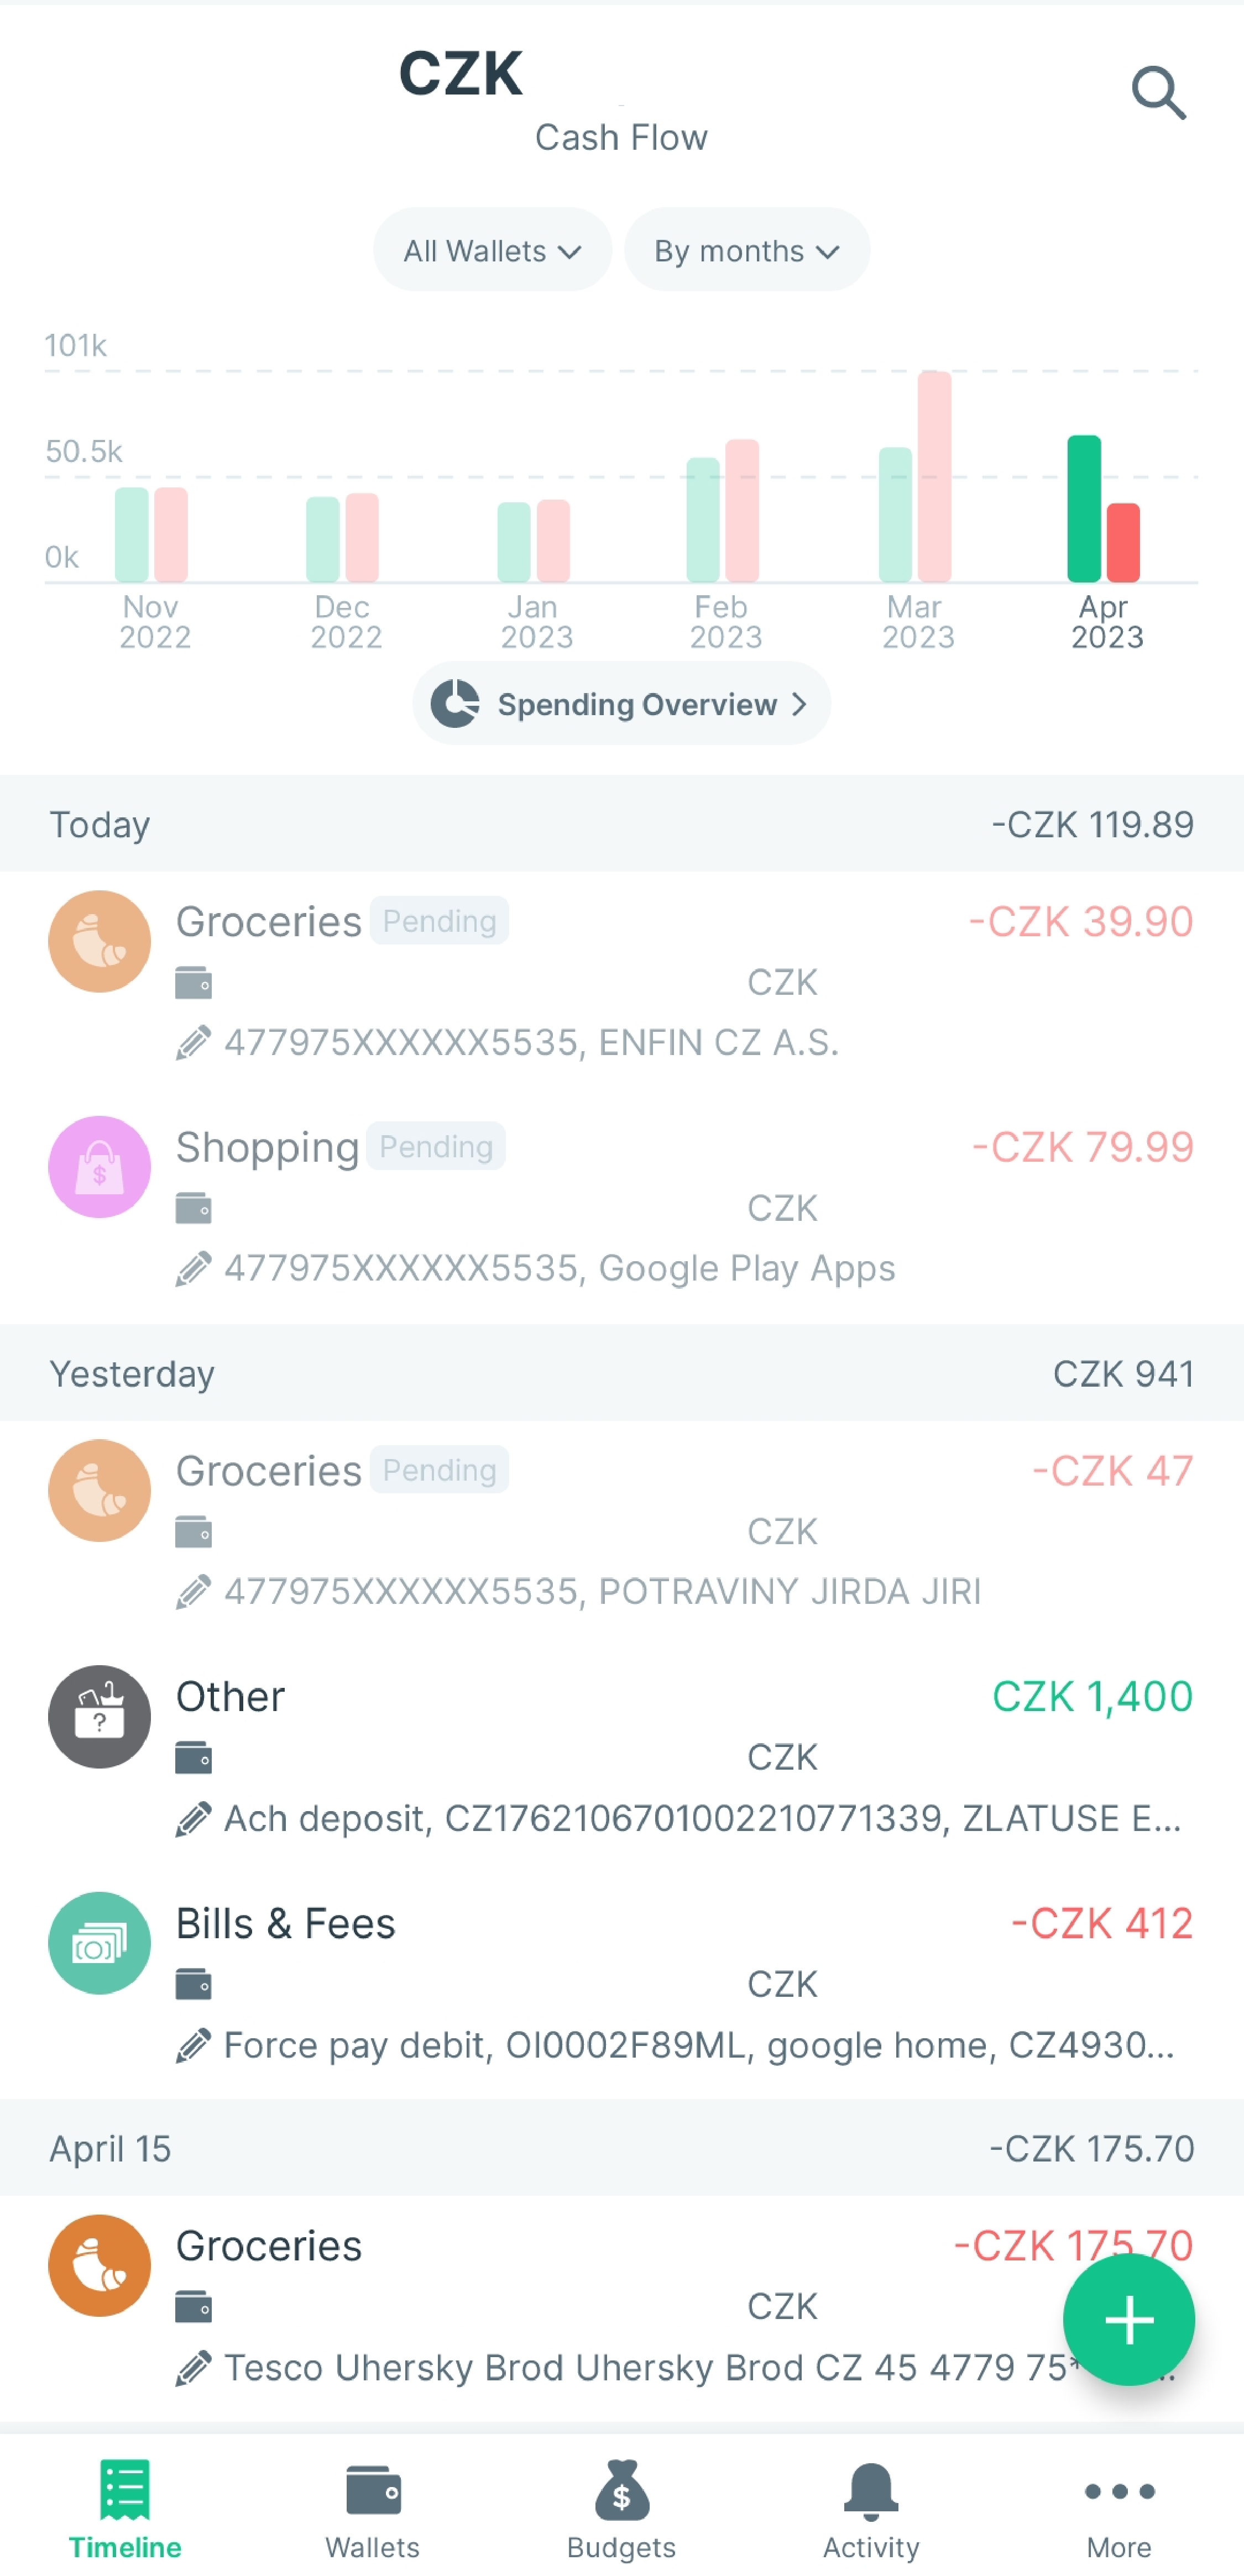
\includegraphics[height=10cm]{spendeecropped.pdf}
    \caption{Aplikace Spendee souhrn výdajů.}
    \label{fig:speende1}
  \end{minipage}
  \hfill
  \begin{minipage}[b]{0.4\textwidth}
    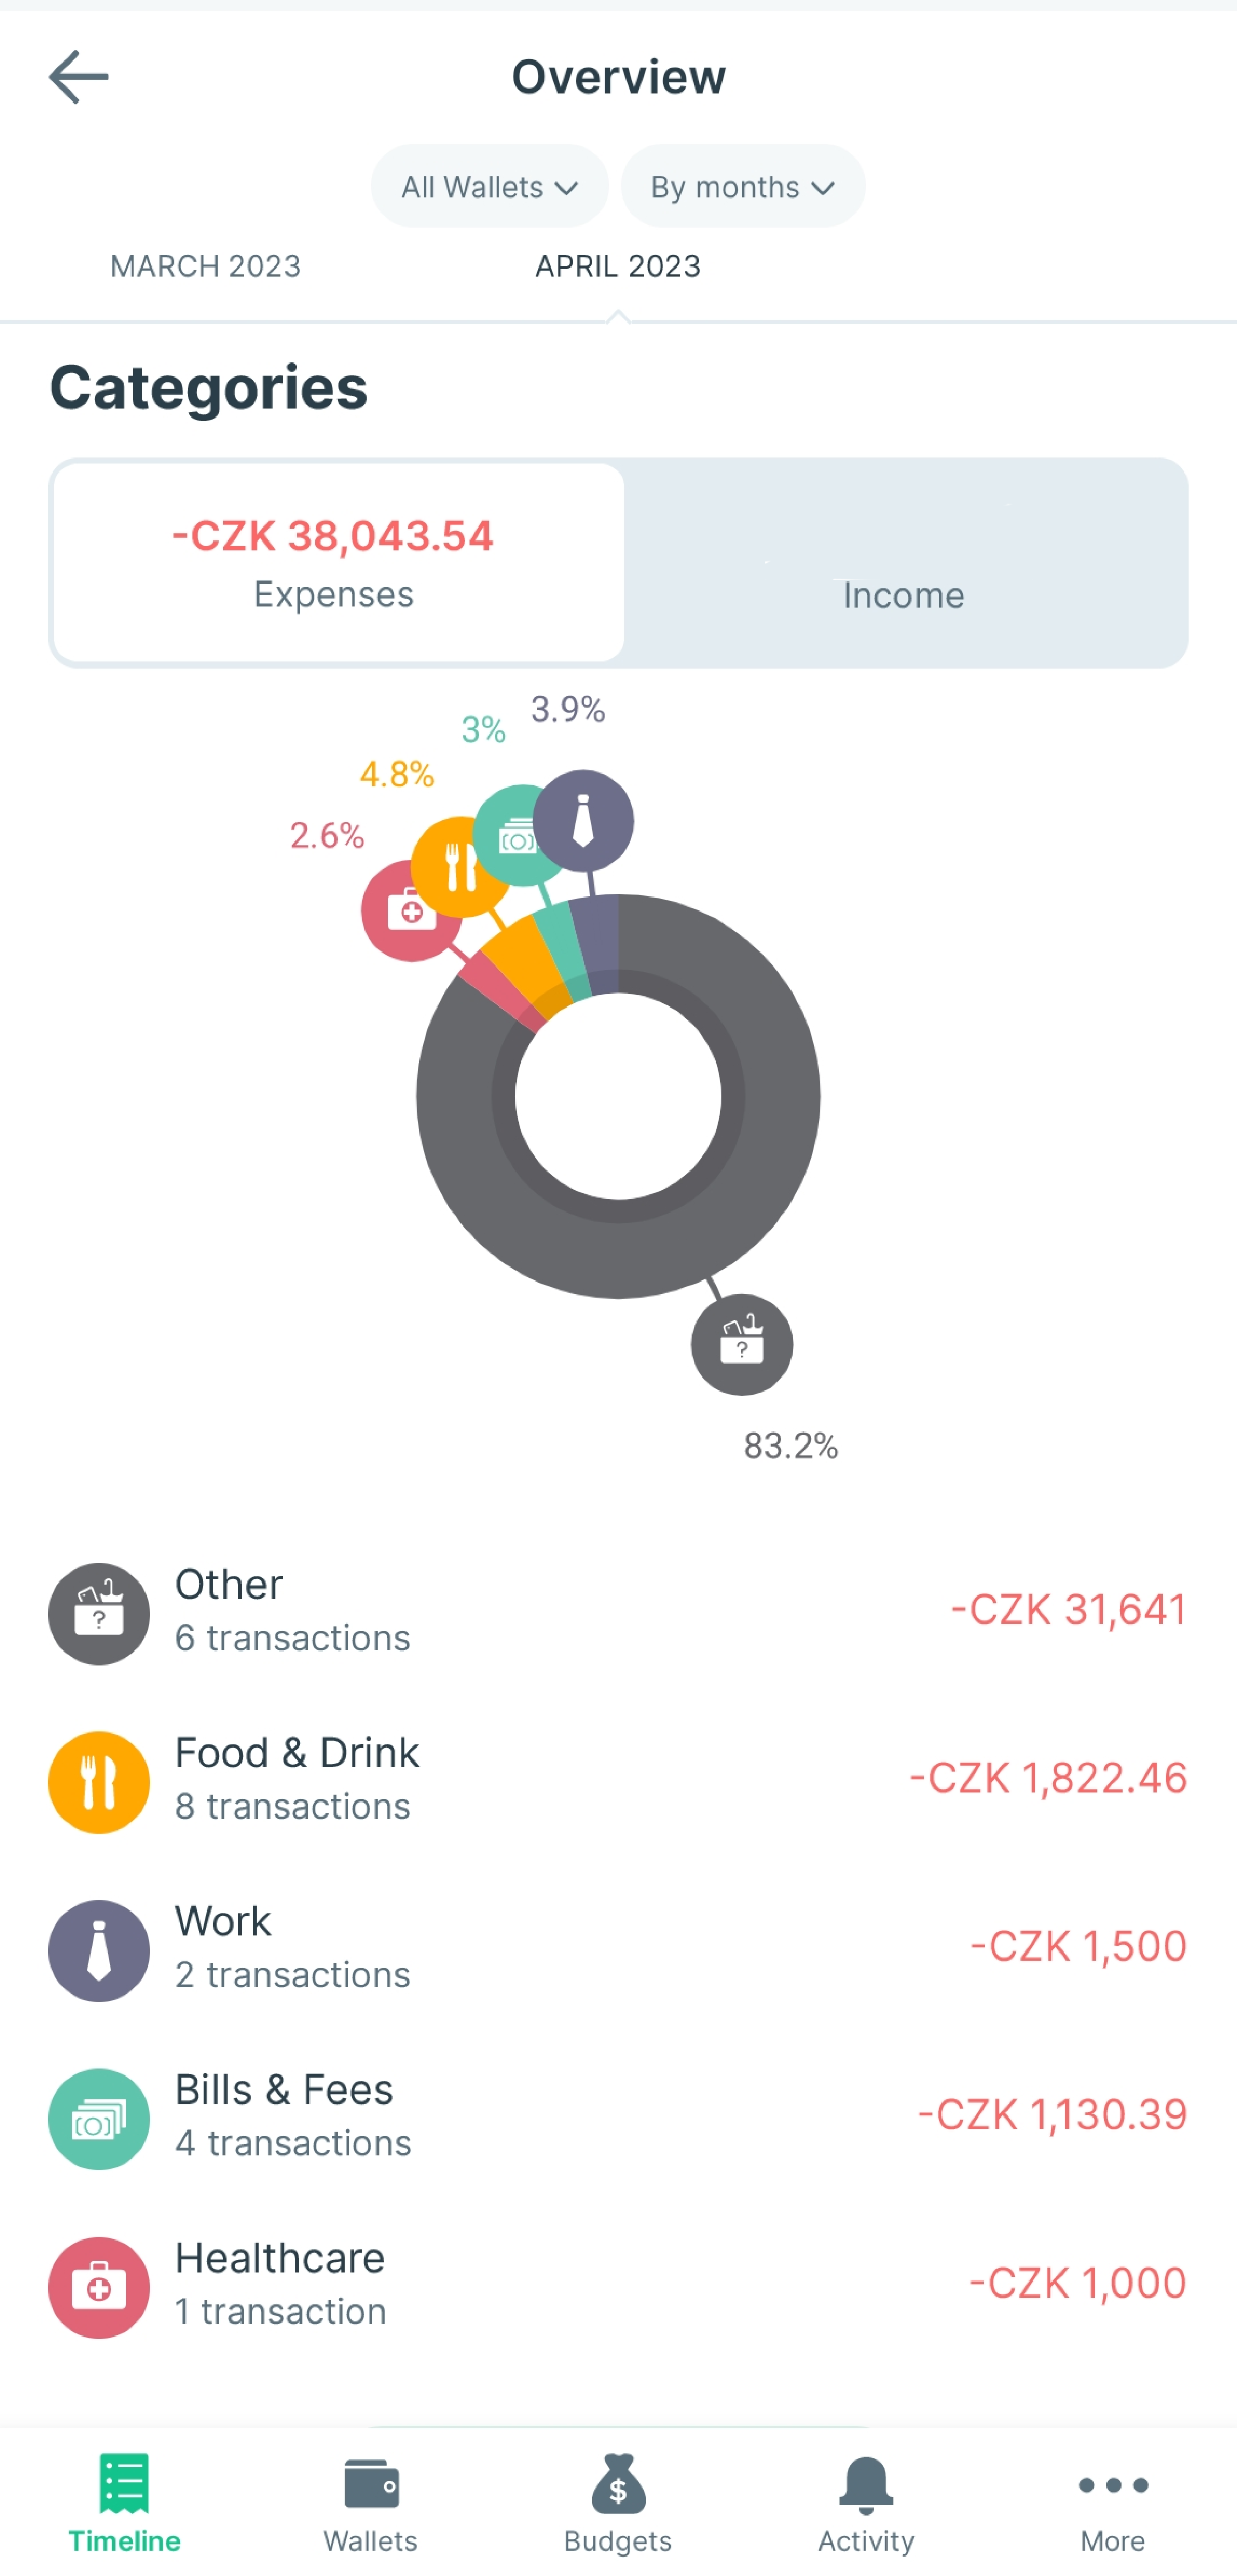
\includegraphics[height=10cm]{obrazky-figures/spendee1.pdf}
    \caption{Aplikace Spendee souhrn graf.}
    \label{fig:speende2}
    
  \end{minipage}
\end{figure}
\subsection*{YNAB (You need a~budget)}

YNAB\footnote{\url{https://www.ynab.com/}} (You Need A~Budget) je aplikace pro správu osobních financí, která pomáhá uživatelům získat kontrolu nad svými financemi a~plánovat své výdaje. Tato aplikace se zaměřuje na tzv. pravidlo 4 kroků, které zní:
\begin{itemize}
    \item Přiřazuj každý dolar k~nějakému výdaji.
    \item Sleduj všechny výdaje.
    \item Stanov si priority pro výdaje.
    \item Zůstávej v~mezích svého rozpočtu.
\end{itemize}
YNAB pomáhá uživatelům žít podle svého rozpočtu a~plánovat si své výdaje s~předstihem, což umožňuje snížit stres z~financí a~dosáhnout finanční svobody.
Aplikace stojí 15\$ měsíčně a~nemá žádnou neplacenou verzi. Do aplikace si postupně zapíšete svoje měsíční výdaje a~následně vás aplikace požádá o~doplnění transakcí. Aplikace také nabídne napojení na API banky, ale v~seznamu se nenachází žádná česká banka. Aplikace umožní nahrání CSV souboru pouze přes webové prostředí, které je značně nepřehledné a~je nutné upravit CSV soubor, který nám poskytne banka. Na obrázku \ref{fig:ynab} můžeme vidět modální okno pro nahrání souboru.
\begin{figure}[ht]
    \centering
    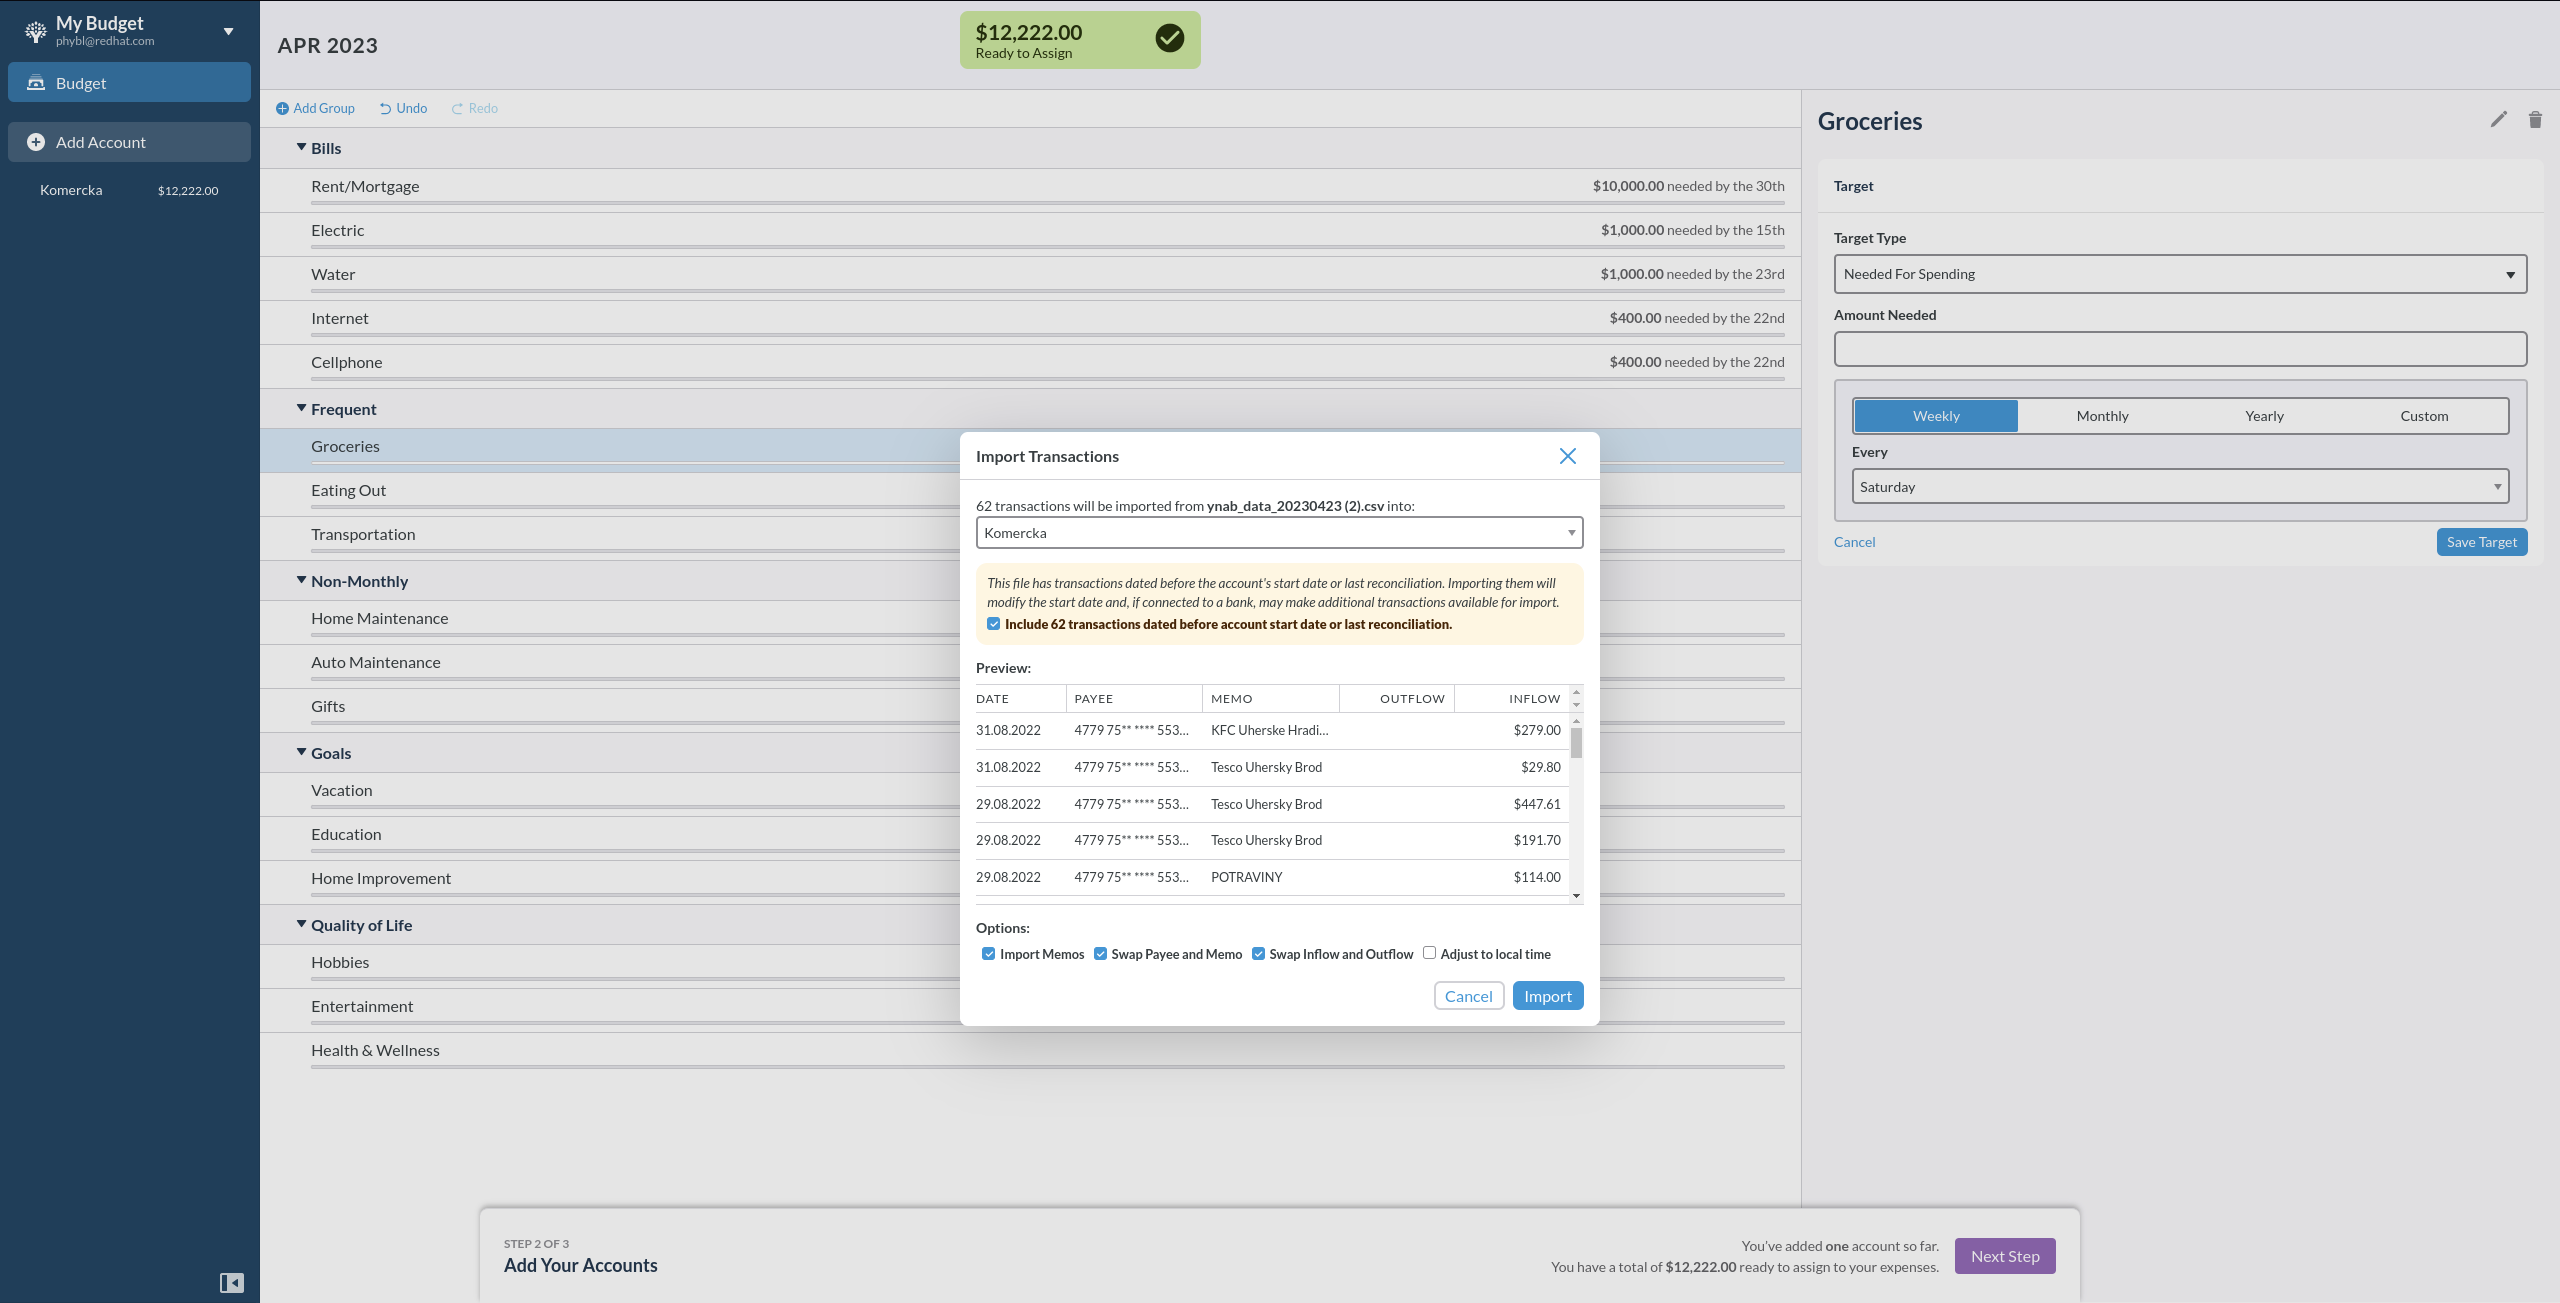
\includegraphics[width=\textwidth]{obrazky-figures/ynab.png}
    \caption{Nahrávání výpisu do YNAB.}
    \label{fig:ynab}
\end{figure}
\section{Webové aplikace}

Webové aplikace jsou programy, které běží v~internetovém prohlížeči uživatele a~umožňují interakci s~obsahem na internetu. Tyto aplikace jsou stále populárnějšími, neboť jsou snadno dostupné, nemusí se instalovat a~mohou být používány na jakémkoli přístroji s~připojením k~internetu. Ve světě financí si lidé zvykli na internetové bankovnictví. Byla to první možnost komunikace s~bankou bez bankéře a~lidé je používají i~dnes, a~právě proto si myslím, že v~dnešní době dává smysl mít finanční aplikace dostupné na webu.

\subsection{Mint}
Aplikace Mint\footnote{\url{https://mint.intuit.com/}} je nástroj pro správu financí, která slouží ke sledování a~správě vašich osobních financí. Tato aplikace vám umožňuje propojit vaše bankovní účty, kreditní karty, investiční účty a~další finanční účty, aby vám poskytla celkový přehled o~vašich finančních aktivitách. Mint vám umožňuje sledovat vaše příjmy a~výdaje, kategorizovat transakce a~sledovat vaše výdaje v~reálném čase. Aplikace vám také poskytuje různé nástroje a~funkce, např. upozornění na zůstatek na účtu, sledování kreditního skóre, plánování rozpočtu a~investiční nástroje. Webová aplikace není dostupná v~České republice, nepodporuje banky působící na tuzemském trhu, ale v~zahraničí je velmi oblíbená, podobně jako Spendee. Také zde přidáváme své transakce po jedné a~následně vidíte grafy, kde se co dá zlepšit. Aplikace působí přehledně.

\subsection{Goodbudget}
Goodbudget\footnote{\url{https://goodbudget.com/}} je aplikace pro správu osobních financí, která pomáhá uživatelům plánovat své výdaje pomocí obálkové metody. Tato metoda spočívá v~tom, že uživatelé si přiřadí k~jednotlivým kategoriím své výdaje do obálky s~určitými peněžními limity a~snaží se tyto limity nepřekročit. Goodbudget umožňuje uživatelům sledovat, kolik peněz jim zbývá v~každé kategorii, a~tím koordinovat následující výdaje. Aplikace také umožňuje sdílet účty s~rodinou.
Webová aplikace nabízí jednoduché nahrání CSV souboru, dokonce ve webovém prostředí nabídne úpravu CSV souboru. Moje testovací výpisy z~Komerční banky, ale byly velmi špatně rozpoznány a~ani v~jedné transakci nebyla správná hodnota transakce, jak můžeme vidět na obrázku \ref{fig:goodbudget}
\begin{figure}[ht]
    \centering
    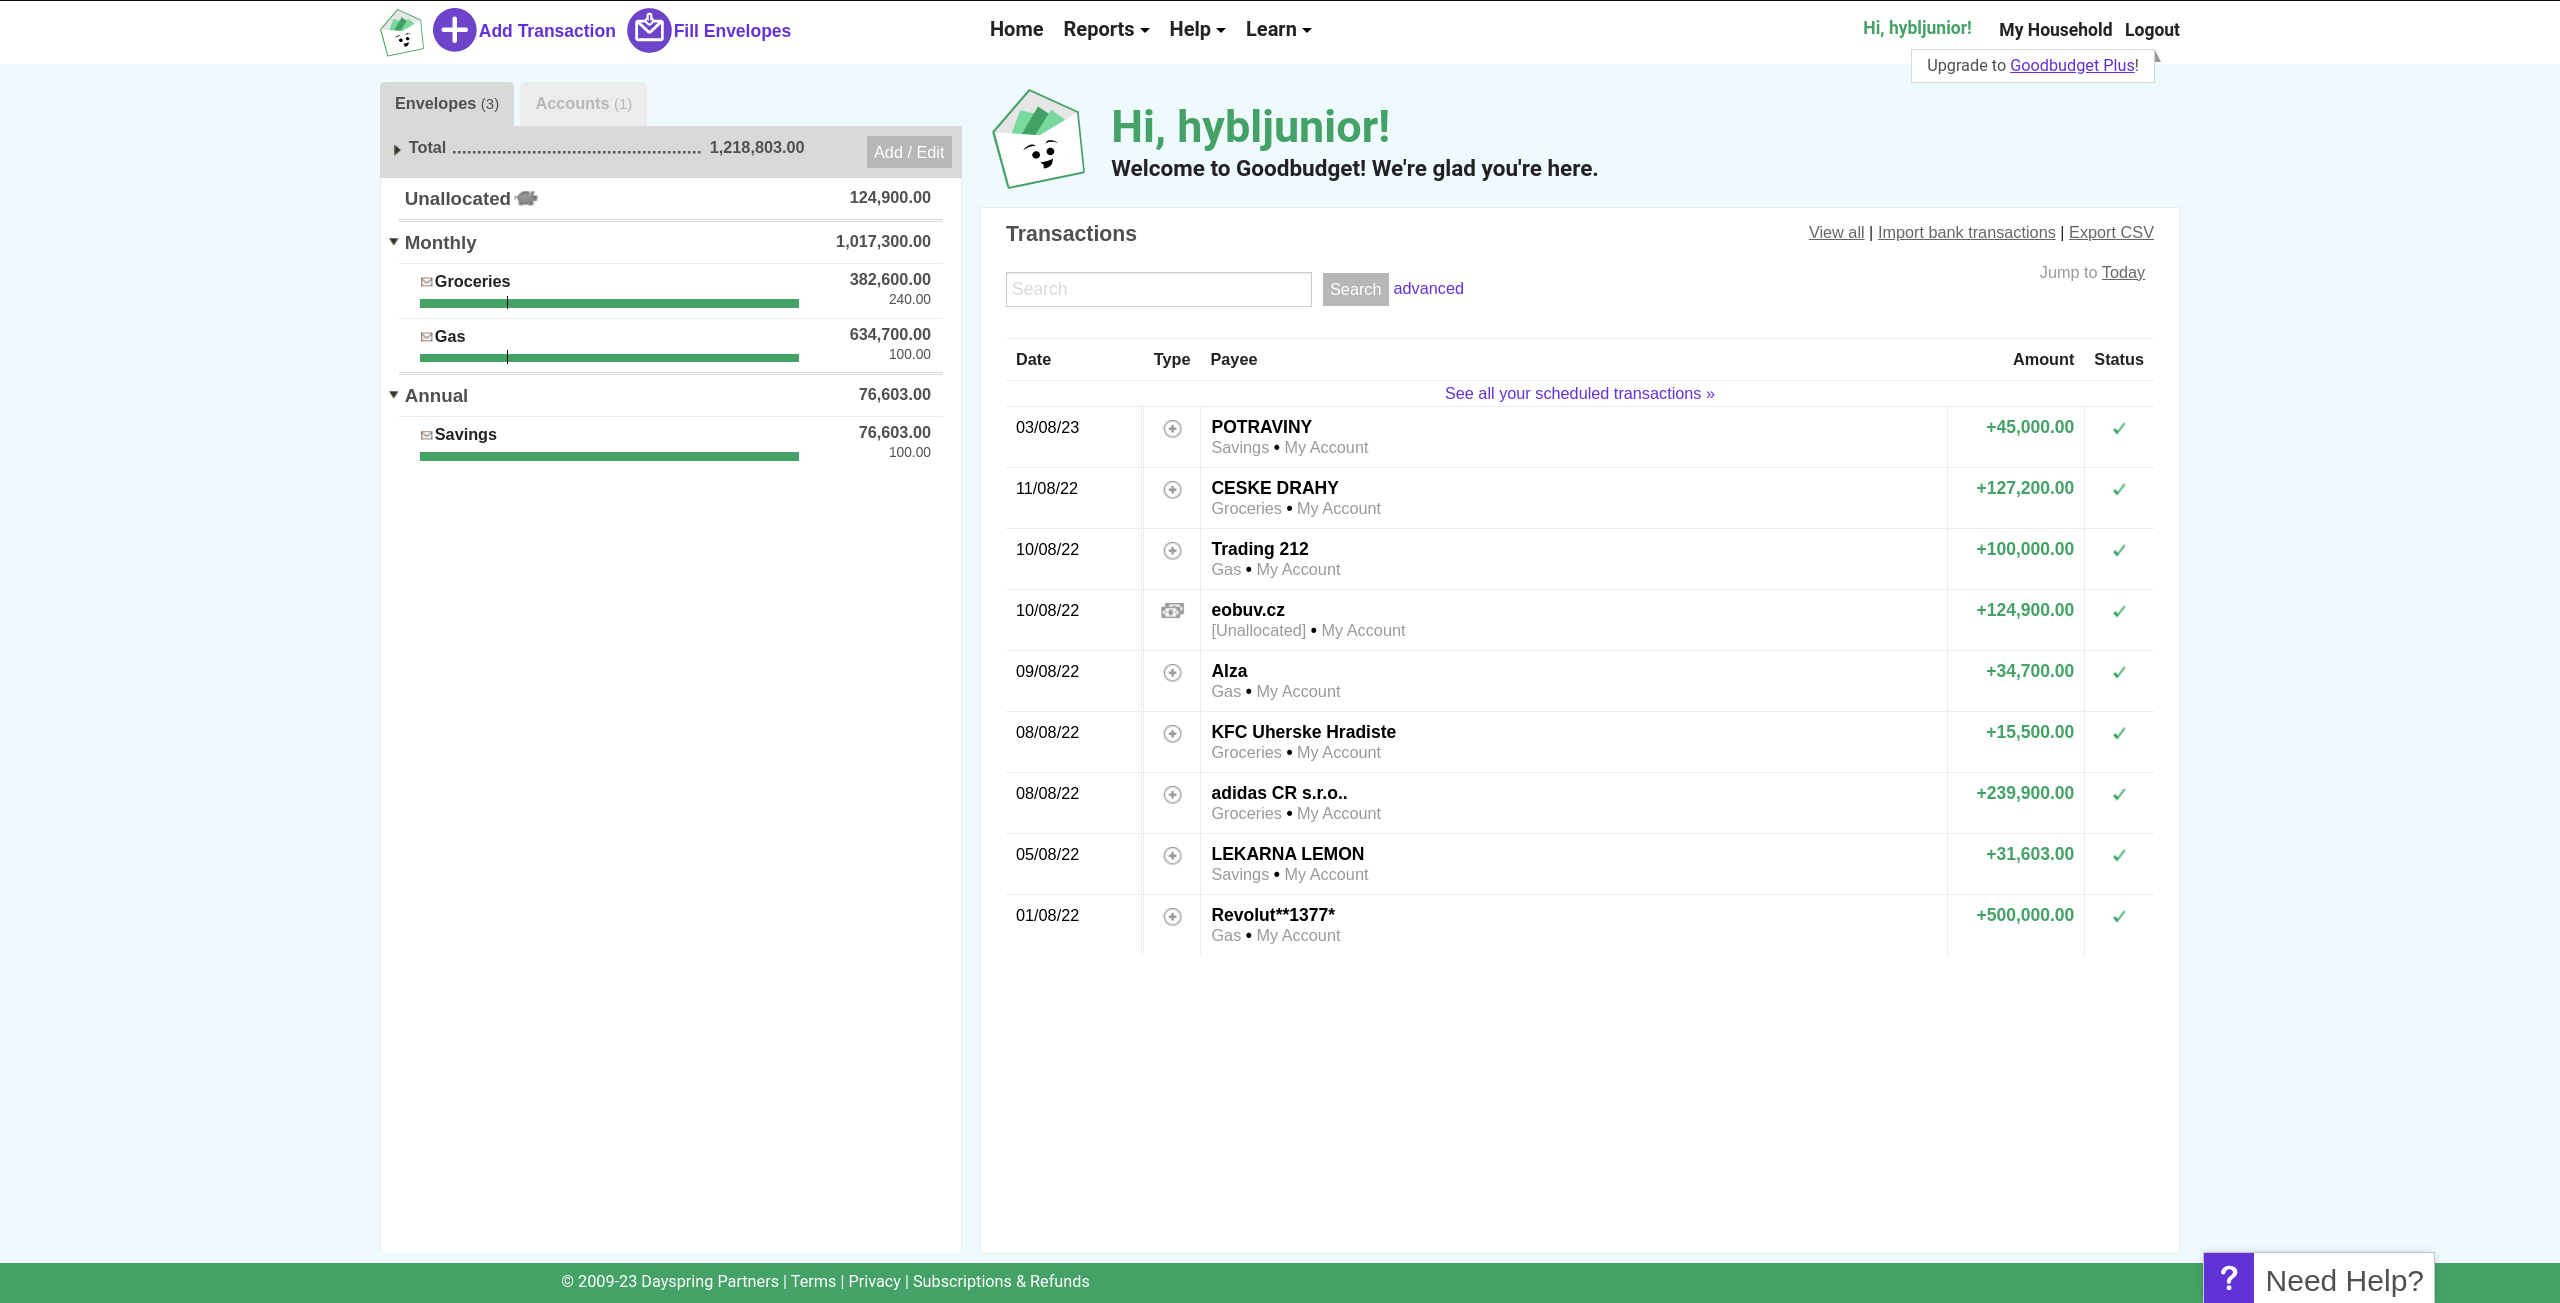
\includegraphics[width=\textwidth]{obrazky-figures/goodbudget.png}
    \caption{Přehled transakcí v~Goodbudget.}
    \label{fig:goodbudget}
\end{figure}

\section{Závěr}
Shrnul jsem zde 4 aplikace pro správu osobních financí, které jsou v~dnešní době dle různých internetových magazínů nejpopulárnější a~také jsem si je mohl osobně vyzkoušet. Největší negativa těchto aplikací jsou uživatelská nekomfortnost při nahrávání vašich výpisů a~placení měsíčních poplatků. Z~této analýzy jsem dospěl k~závěru, že v~České republice chybí nekomerční aplikace pro kategorizaci vašich výdajů.

\chapter{Použité technologie}
V~této kapitole budou prezentovány informace o~použitých technologiích při vývoji aplikace a~důvody pro volbu daných technologií.
\section{Webové frameworky}

Dny, kdy se weby psaly pouze v~HTML a~CSS jsou již za námi. Ani s~přidaným Javascriptem na rozpohybování HTML elementů, již dnes plnohodnotnou webovou aplikaci nenapíšeme jednoduše. Z~webů se staly robustnější aplikace tzv. webové aplikace, které potřebují složitější logiku a~tak vznikly webové frameworky.

Webové technologie jsou jedny z~nejrychleji vyvíjejících technologií v~oblasti informačních technologií. Webové aplikace jsou v~podstatě aplikace na architektuře klient--server, kterou si popíšeme později. Běží ve webovém prohlížeči a~komunikují přes protokol HTTP. Novým standardem pro webové aplikace se staly webové frameworky, které nám ulehčují jejich vývoj.

\subsection{Single--page weby}
Single--page aplikace je webová aplikace, jejíž veškerý obsah je tvořen jedinou stránkou. Uživatel této aplikace nemusí po každém kliknutí na nový obsah stránky stahovat celou stránku znovu, stačí pouze načíst obsah, který potřebujeme obnovit~\cite{barborakoouskov_2020_co}.
Single--page aplikace se v~dnešní době dělají pomocí javascriptových frameworků a~knihoven. Na obrázku \ref{graf:stack} můžeme vidět 6 nejvyhledávanějších a~nejvyužívanějších webových frameworků v~roce 2022~\cite{stackoverflow}:

\begin{figure}[H]
    \centering
    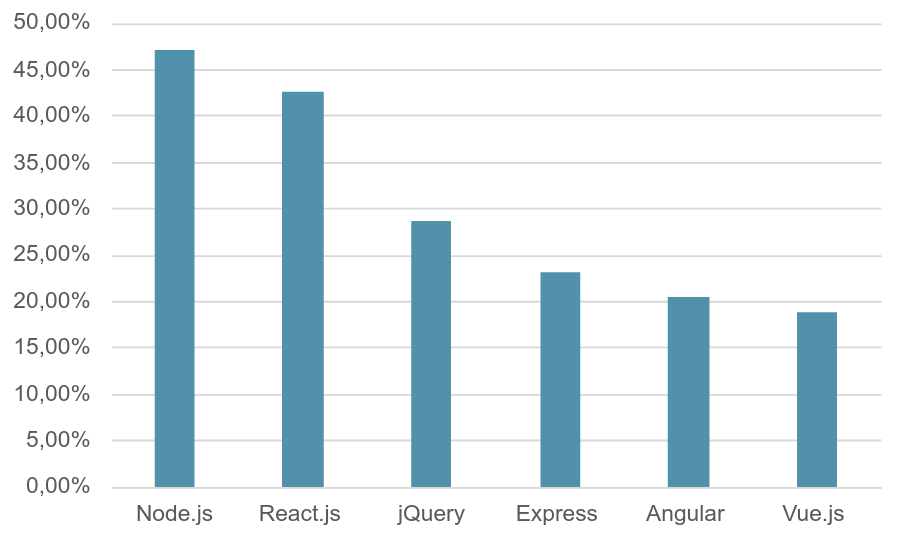
\includegraphics[width=\textwidth]{obrazky-figures/table1.png}
    \caption{Popularita webových frameworků v~roce 2022 \cite{stackoverflow}.}
    \label{graf:stack}
\end{figure}
Všechny si postupně rozebereme v~následujících kapitolách.
\subsection{Node.js}
Node.js\footnote{\url{https://nodejs.org/en}} umožňuje programátorům používat JavaScript na straně serveru, což znamená, že lze vytvářet komplexní webové aplikace pomocí jediného jazyka -- JavaScriptu~\cite{mal_2010_nodejs}. Node.js je ideální pro tvorbu rychlých, škálovatelných a~vysoce výkonných webových aplikací, API nebo serverových služeb~\cite{barborakoouskov_2020_pro}. V~předchozích letech Node.js nebyl považován za webový framework, ale v~dnešní době ho již mnoho vývojařů považuje za plnohodnotný framework a~tvoří základ pro vytváření dalších webových frameworků, jako například Express.js, který poskytuje další vrstvu abstrakce. V~mé práci by volba Node.js dávala smysl pouze při volbě jazyka JavaScript pro serverovou část aplikace.

\subsection{React.js}
React.js\footnote{\url{https://react.dev/}} je javascriptová knihovna pro tvorbu uživatelského rozhraní. Vytvořena byla zaměstnancem firmy Facebook a~je dále rozvíjena firmou Meta (dříve Facebook)~\cite{fedosejev2015react}. Hlavní výhodou a~také důvodem, proč v~této práci bude použit React je virtuální DOM (Document Object Model), díky kterému může aplikace rychle reagovat na změny v~datovém modelu a~držet přitom stabilní výkon aplikace. Další skvělou výhodou je jedna z~největších komunitních základen a~rozsáhlá dokumentace. Správa stavů a~synchronizace aplikace s~datovým modelem je zde implementována přívětivě.

\subsection{jQuery}
jQuery\footnote{\url{https://jquery.com/}} je javascriptová knihovna s~širokou podporou prohlížečů, která klade důraz na interakci mezi JavaScriptem a~HTML. Byla vytvořena v~roce 2006\footnote{\url{https://blog.jquery.com/2006/08/26/jquery-10/}} a~jedná se tak o~nejstarší knihovnu v~našem výběru a~hlavně kvůli stáří ji nechci ve své práci používat.

\subsection{Express}
Express\footnote{\url{https://expressjs.com/}} je populární open--source framework pro Node.js, který umožňuje vytvářet webové aplikace a~API. Express poskytuje jednoduché a~minimalistické rozhraní pro vytváření serverových aplikací. Express je serverový javascriptový framework a~protože bude náš server hodně pracovat s~úpravou dat Javascript není úplně správná volba, proto ho nebudeme v~naší práci používat.

\subsection{Flask}
Flask\footnote{\url{https://flask.palletsprojects.com/en/2.2.x/}} je open--source webový framework pro programování webových aplikací v~jazyce Python. Je to lehký framework, který nabízí jednoduchou a~elegantní architekturu, což umožňuje programátorům rychle a~snadno vytvářet webové aplikace. 
Mezi výhody použití Flasku patří jeho jednoduchá architektura, která umožňuje programátorům rychle se s~ním seznámit a~začít s~vývojem webových aplikací. Flask také umožňuje rozšiřování a~přizpůsobení podle potřeb vývojářů, což z~něj činí vhodný framework pro malé a~střední webové projekty. Flask také obsahuje rozsáhlou dokumentaci a~silnou komunitu, což umožňuje vývojářům rychle najít řešení problémů. V~naší aplikace bude Flask běžet na serveru a~díky jazyku Python nám umožní zprovoznění umělé inteligence přes knihovnu PyTorch. Python je též skvělý a~použitelný pro dolování z~dat a~práci s~řetězcem textu.

\subsection{Angular}
Angular\footnote{\url{https://angular.io/}} je open--source webový framework vyvíjený společností Google, který slouží k~vývoji moderních a~dynamických webových aplikací. Angular využívá jazyk TypeScript, který umožňuje psát kód s~větší jistotou, což zlepšuje jeho čitelnost a~údržbu.
Mezi nevýhody použití Angularu patří jeho složitější syntaxe, která může být pro programátory náročná. Angular také vyžaduje větší množství zbytečného kódu a~konfigurace než jiné webové frameworky, což může vést k~většímu objemu kódu a~zvýšené složitosti aplikace. 

\subsection{Vue.js}
Vue.js\footnote{\url{https://vuejs.org/}} je moderní a~open--source frontendový framework pro vývoj webových aplikací a~uživatelských rozhraní (UI). Byl vytvořen v~roce 2014 a~jeho hlavním tvůrcem je Evan You\footnote{\url{https://vuejs.org/about/faq.html}}. Jeho cílem je poskytnout jednoduchý a~flexibilní framework pro vývoj moderních webových aplikací. Hlavní nevýhodou tohoto frameworku je malá komunita, což může vést k~menšímu počtu návodů, knihoven a~rozšíření.

\section{Architektura}
Správná architektura webové aplikace může výrazně ovlivnit úspěch a~celkovou kvalitu aplikace. Tím pádem je důležité pečlivě zvážit při návrhu architektury webové aplikace různé faktory jako jsou potřeby uživatelů, požadavky na výkon a~škálovatelnost, zabezpečení a~další. Celá architektura je postavena na konceptu Třívrstvé architektury. Následující kapitola je převzata z~\cite{rouse_2021_threetier}.
\subsection{Třívrstvá architektura}
Je to metoda rozdělení architektury aplikace do tří nezávislých vrstev -- prezentační, aplikační a~datová. Každá má svůj specifický úkol. Na obrázku \ref{fig:trivstva} můžete vidět diagram propojení celé architektury.


\begin{figure}[ht]
\centering
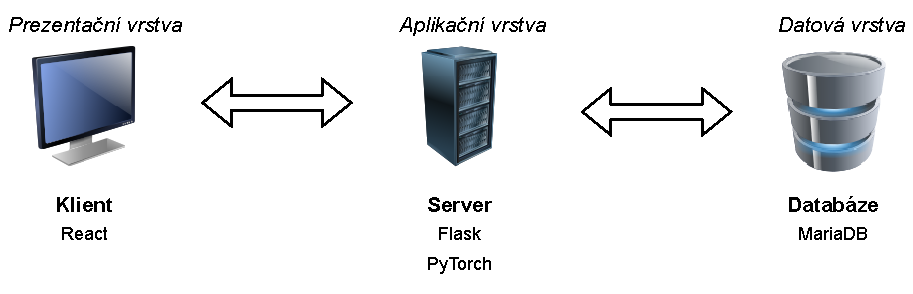
\includegraphics[width=\textwidth]{./obrazky-figures/server_klient.pdf}
\caption{Třívrstvá architektura.}
\label{fig:trivstva}
\end{figure}

\subsubsection{Prezentační vrstva}
Jediná vrstva se kterou interaguje uživatel, ten zadá vstupní data a~zobrazí se mu výstupní data ve srozumitelné formě. Zahrnuje různé typy UI prvků, jako jsou formuláře, tlačítka, seznamy, tabulky a~další. Tyto prvky umožňují uživatelům zadávat data, procházet seznamy a~zobrazovat výsledky svých akcí. Prezentační vrstva má také vliv na celkový vzhled a~pocit z~aplikace. Vývojáři musí zvážit různé faktory, jako jsou typy uživatelů, účel aplikace, obecné návyky uživatelů a~další faktory, při navrhování uživatelského rozhraní. V~dnešní době se také klade důraz na přístupnost a~zohlednění přístupu pro lidi s~nějakým postižením. Prezentační vrstva je zastoupena v~mé práci klientem a~bude implementována frameworkem React.js.
\subsubsection{Aplikační vrstva}
Tato vrstva má na starosti logiku celé aplikace a~stará se o~zpracování dat. Přijímá požadavky prezentační vrstvy a~ty dále zpracovává. Hlavním úkolem aplikační vrstvy je zpracování požadavků uživatelů. Aplikační vrstva je v~mé práci zastoupena serverem a~bude implementována frameworkem Flask. V~této vrstvě bude probíhat kategorizace transakcí pomocí modelu umělé inteligence s~knihovnou PyTorch.
\subsubsection{Datová vrstva}
Datová vrstva je nejnižší vrstva architektury, která se stará o~ukládání a~získávání dat z~databáze. Hlavním úkolem datové vrstvy je zajistit, aby data byla ukládána bezpečně, konzistentně a~efektivně, a~aby byla snadno dostupná pro další zpracování v~aplikaci. Správná funkčnost datové vrstvy je zásadní pro celkovou funkčnost aplikace, protože zajišťuje, že data jsou uložena a~zpracována správným způsobem. V~této vrstvě budu používat MariaDB.
\subsection{Server}
Na serveru budu využívat webový framework Flask, který nabízí celou řadu užitečných funkcionalit, včetně efektivní práce s~textovými řetězci a~schopnosti stavět API ve formě logických celků. Python disponuje rozsáhlou knihovnou funkcí a~modulů jako např. knihovnu pro práci s~umělou inteligencí PyTorch.
\subsection{Klient}
Pro klienta budu využívat webový framework React. Vybral jsem si jej zejména díky komunitní základně a~využití virtuálního DOM modelu, který se bude hodit při tvorbě aplikace a~zjednoduší některé činnosti. Díky propojení přes API nemusím řešit žádnou kompatibilitu mezi frameworky na serveru a~klientu.
\subsection{Databáze}
Správná volba databázového systému je klíčová pro úspěšné dokončení projektu. MariaDB\footnote{\url{https://mariadb.com/}} je relační databázový systém, který vznikl v~roce 2009 jako fork MySQL\footnote{\url{https://www.mysql.com/}}, a~díky svým vlastnostem a~výhodám si získal popularitu mezi uživateli i~vývojáři. Je to open-source software s~velkou komunitou uživatelů a~vývojářů, což umožňuje uživatelům upravovat a~rozšiřovat systém podle svých potřeb. MariaDB má silnou reputaci na trhu databázových systémů. MariaDB obsahuje několik vylepšených funkcí, které nejsou v~MySQL k~dispozici např. pokročilé dotazy, lepší indexování, optimalizaci dotazů, nové úložiště pro datové typy a~další~\cite{mariadb}.

\section{Síťová komunikace}
V~následující části budu popisovat, jakými protokoly a~formáty server a~klient komunikují mezi sebou. Přenos dat je šifrován přes HTTPS, data se posílají ve formátu JSON.
\subsection{HTTP}
HTTP (Hypertext Transfer Protocol) je protokol aplikační vrstvy. Dnes je hlavně používaný na přenos dat po síti. Základní princip tohoto protokolu je odesílání požadavku a~očekávání odpovědi ze serveru. Protokol si neukládá jednotlivé požadavky, to značí že je bezstavový~\cite{a2021_ibm}. Bezstavovost budeme řešit pomocí autentizačních hlaviček s~tokeny. 
\subsubsection{Základní HTTP metody}
HTTP metody jsou používány k~určení, jakým způsobem bude zpracován požadavek odeslaný klientem na server. Při odesílání na adresu se přidávají k~metodám také informace o~verzi protokolu a~různé hlavičky. Existují čtyři základní metody~\cite{gourley2002http}:
\begin{itemize}
\item \texttt{GET} -- Odesílá požadavek na získání informací na serveru.
\item \texttt{POST} -- Odesílá informace, které mají být zpracovány na serveru.
\item \texttt{PUT} -- Odesílá kompletní zdrojový soubor na server.
\item \texttt{DELETE} -- Odesílá informace, které se mají smazat na webovém serveru.
\end{itemize}
Dále existují také další metody, jako např. \texttt{HEAD}, \texttt{OPTIONS}, \texttt{TRACE} nebo \texttt{CONNECT}, které se používají v~speciálních případech, v~mé práci nebudou potřeba.
Při přijímání odpovědi na požadavek dostáváme odpověď ve formě číselného kódu:
\begin{itemize}
    \item 1xx -- informační charakter,
    \item 2xx -- operace schválena, akceptována,
    \item 3xx -- operace přesměrování, potřeba dalších úprav pro splnění požadavku,
    \item 4xx -- operaci nelze splnit,
    \item 5xx -- chyba na straně serveru,
\end{itemize}

\subsection{HTTPS}
HTTPS (Hypertext Transfer Protocol Secure) je rozšíření již uvedeného aplikačního protokolu HTTP. Hlavní nevýhoda původního protokolu byla možnost sledování a~čtení komunikace mezi serverem a~klientem a~takovou vlastnost u~aplikace zaměřenou na finance nechceme.
U~HTTPS jsou použity kryptovací protokoly s~asymetrickým šifrováním. Toto šifrování chrání komunikaci mezi klientem a~server. Tato technologie zabraňuje podvržení zpráv i~jejich čitelnost někým jiným než serverem a~klientem, kteří mezi sebou tuto komunikaci vedou~\cite{rfchttps}.

\subsection*{Application Programming Interface}

API (Application Programming Interface) je komunikační rozhraní, které používají webové služby pro komunikaci mezi servrem a~klientem.
API jednoznačně odděluje prezentační část od aplikační a~dovoluje napojit webovou i~mobilní aplikaci pomocí stejného rozhraní.
Mezi nejpoužívanější architekturu patří REST.
\subsubsection{REST API}
REST (Represational State Transfer) komunikuje prostřednictvím protokolu HTTP. Díky tomu může využívat již implementované hlavičky, metody, tělo a~stavové kódy. Základní HTTP metody (GET, POST, PUT a~DELETE) se přetransformují na CRUD (Create, Read, Update a~Delete) operace, které zprostředkuje server~\cite{restapibook}:
\begin{itemize}
\item \texttt{POST} $\rightarrow$ Create -- Odesílá požadavek na vytvoření dat.
\item \texttt{GET} $\rightarrow$ Read -- Posílá zpátky informace o~datech.
\item \texttt{PUT} $\rightarrow$ Update -- Odesílá požadavek na úpravu dat.
\item \texttt{DELETE} $\rightarrow$ Delete --  Odesílá požadavek na smazání dat.
\end{itemize}
REST architektura má obecně definované principy~\cite{restapibook}, které jsem se snažil dodržet v~mé práci:
\begin{itemize}
    \item Jednotné rozhraní
    \item Architektura klient--server
    \item Bezstavová logika
    \item Vrstvená architektura
    \item Kód na vyžádání
    \item Ukládání dat do cache
\end{itemize}

\subsection{JSON}
JSON (JavaScript Object Notation) je formát pro přenos dat. Jeho syntaxe je založena na JavaScriptových objektech a~polích a~umožňuje reprezentovat data ve formátu hierarchických stromů. Data jsou uloženy ve formátu \texttt{\{"klíč":"hodnota"\}}. Tento formát je čitelný jak pro stroje, tak i~pro lidské oko~\cite{rfcjson}.

\section{Autentizace}
Autentizace neboli ověření uživatelovy identity lze provádět mnoha způsoby. V~mé aplikaci jsem zvolil klasický způsob ověření, a~to přes uživatelův email a~heslo. Tento email bude pro každého uživatele taktéž jedinečný identifikátor. Kromě tohoto klasického způsobu se stále více využívá biometrie, díky její rychlosti a~přesnosti. U~bankovních aplikací jsou také rozšířené PIN kódy, bezpečnostní kódy a~nebo osobní otázky. V~rámci zvýšení zabezpečení může společnost používat i~více druhů autentizace a~tak zvýšit bezpečnost na úkor uživatelské přívětivosti~\cite{dasgupta2017advances}.

\subsection*{JWT token}
JWT (JSON Web Token) je internetový standard pro formát tokenu, který lze použít pro autentizaci a~autorizaci. 
Jedná se o~kompaktní a~samostatně přenositelný způsob přenosu informací o~uživateli mezi různými částmi aplikace. JWT obsahuje zakódované informace o~uživateli v~JSON formátu, které jsou podepsané digitálním podpisem pro zajištění integrity dat~\cite{rfc7519}.
Po autentizaci se vytvoří na serveru token (API endpointem \texttt{/token}), který pomocí API rozhraní přijme prohlížeč a~uloží si ho do Local Storage. Local Storage (Web Storage) je jedna z~funkcionalit moderních webových prohlížečů, která dovoluje aplikacím ukládat data na počítači uživatele. Tato data se ukládají přímo do paměti prohlížeče a~jsou k~dispozici i~po restartu prohlížeče~\cite{shwetank_2013_web}. Při každém dalším volání API se do HTTP hlavičky přidá řádek s~autentizačním tokenem. Tak server pozná o~jakého uživatele se jedná a~podle toho uzpůsobí dál svoje chování.


\chapter{Analýza požadavků}
V~následující kapitole budou popsány jaké formáty bankovní společnosti nabízejí.
\section{Formáty souborů bank}
\label{chap:formaty}
Při zkoumání výpisů formátu aplikace jsem kontaktoval všechny přední banky v~České republice formou telefonického hovoru nebo emailem a~zeptal jsem se, jaké formáty nabízí pro výpisy. Základním formát souboru je PDF, ten nabízí všechny bankovní společnosti. Tento formát se velmi špatně čte z~pohledu automatizovaného procesu programem. Strojově čitelné formáty pro programy jsou třeba CSV nebo XML. Dle mého průzkumu minimálně jeden z~těchto formátů poskytuje každá banka působící v~ČR. Ze získaných informací jsem složil tabulku \ref{tabulkabank}. V~tabulce můžeme vidět, jaká banka které formáty používá.

\begin{center}
\begin{table}[h]
\begin{tabular}{ |c| c| c| c| c| c| }
\hline
\textbf{Bankovní společnost} & \textbf{CSV}  & \textbf{CSV kódování} & \textbf{XML}  & \textbf{XML kódování} &  \textbf{PDF} \\ 
\hline
Moneta & \checkmark & UTF--8 BOM & \checkmark & UTF--8 & \checkmark \\ 
\hline
Komerční banka & \checkmark & Windows--1250 & $\times$ & $\times$ & \checkmark \\ 
\hline
Equa & $\times$ & $\times$ & \checkmark & UTF--8 & \checkmark \\  
\hline
Creditas & $\checkmark$ & UTF--8 & \checkmark & UTF--8 & \checkmark \\
\hline
mBank & \checkmark & Windows--1250 & $\times$ & $\times$ & \checkmark \\
\hline
Raiffeisenbank & \checkmark & UTF--8 & $\times$ & $\times$ & \checkmark \\ 
\hline
AirBank & \checkmark & Windows--1250 & $\times$ & $\times$ & \checkmark \\ \hline
ČSOB & $\times$ & $\times$ & \checkmark & UTF--8 & \checkmark \\ 
\hline
Fio & \checkmark & UTF--8 & $\times$ & $\times$ & \checkmark \\ 
\hline
UniCredit bank & \checkmark & Windows--1250 & $\times$ & $\times$ & \checkmark \\ 
\hline
\end{tabular}
\caption{Formáty souborů bank.}
\label{tabulkabank}
\end{table}
\end{center}
V~následujících kapitolách si stručně popíšeme jednotlivé formáty a~představíme, která data budeme využívat.

\subsection*{Formát PDF}
Portable Document Format je formát souboru pro elektronické uložení dokumentu, který byl vyvinut společností Adobe. Je to jeden z~nejpopulárnější formátů pro dokumenty, protože dokáže zobrazit a~uložit dokument v~podobě, ve které bude vypadat stejně nezávisle na softwaru a~hardwaru, kde se prohlíží nebo vytváří. PDF dokumenty jsou často používány pro publikace, prezentace, formuláře a~další dokumenty, které mají být zachovány v~původním formátu, bez nutnosti úprav. PDF dokumenty lze zobrazovat a~tisknout na různých zařízeních, včetně počítačů, tabletů a~chytrých telefonů. PDF formát je otevřený standard a~existuje mnoho různých nástrojů pro tvorbu, úpravu a~zobrazování PDF dokumentů~\cite{iso32000-1}. Strojové čtení PDF dokumentů může být náročné, protože PDF není primárně určen pro strojové zpracování. PDF dokumenty jsou v~podstatě digitální obrazy původních dokumentů, které obsahují text, obrázky a~další prvky, a~ty jsou uloženy v~grafickém formátu.
Existuji technologie, které dokážou strojově číst tyto soubory jako třeba OCR (Optical Character Recognition), ale přesné rozpoznávání znaků může být problematické, pokud jsou v~PDF dokumentu použity různé fonty, velikosti písma nebo pokud jsou texty zakřivené.

\subsection*{Formát XML}
Extensible Markup Language (zkráceně XML) je formát souboru pro značkovací zápis (zápis obohacený o~informace o~struktuře, významu a~zobrazení textu). Vytvořený mezinárodní konsorciem W3C\footnote{\url{https://www.w3.org/}}. XML umožňuje strukturovat data pomocí značek a~atributů, podobně jako HTML. Detailní specifikace tohoto formátu je dostupná z~\cite{RFCXML}.
Nicméně na rozdíl od HTML je XML univerzálnější a~může být použit pro různé typy dat. Neexistuje žádná standardizace mezi bankami a~tak používá každá banka jiné zápisy. XML jde velmi pěkně strojově číst, proto ho využijeme v~naší práci.
\\
Příklad výpisu jedné transakce od Monety:
\begin{lstlisting}[language=XML,breaklines=true]
<transaction id="220610V0385345" other-account-number="PLATBA KARTOU" date-post="2022-06-09" date-eff="2022-06-13" var-sym="4152280774" con-sym="1178" spec-sym="" amount="-24.90" contactless="0" mobile-payment="0">
	<trn-messages type="description">
		<trn-message position="2">ALBERT VAM DEKUJE BRNO CZ</trn-message>
	</trn-messages>
</transaction>
\end{lstlisting}
Příklad výpisu jedné transakce od ČSOB (zkráceno):
\begin{lstlisting}[language=XML,breaklines=true]
<Ntry>
    <NtryRef>20503</NtryRef>
    <Amt Ccy="CZK">154.90</Amt>
    <CdtDbtInd>DBIT</CdtDbtInd>
    <RvslInd>false</RvslInd>
    <Sts>BOOK</Sts>
    <BookgDt>
	<Dt>2023-01-11</Dt>
	</BookgDt>
	<BkTxCd>
		<Prtry>
			<Cd>30000301000</Cd>
			<Issr>Czech Banking Association</Issr>
		</Prtry>
	</BkTxCd>
	<NtryDtls>
		<TxDtls>
		<Refs><AcctSvcrRef>20503</AcctSvcrRef></Refs>
			<BkTxCd>
			<Prtry><Cd>30000301000</Cd>
			<Issr>Czech Banking Association</Issr></Prtry>
			</BkTxCd>
		<RmtInf> <Ustrd>Misto: Penny Mocidla 2369 Uhersky Brod Castka: 154.9 CZK 09.01.2023</Ustrd>
		</RmtInf>
		</TxDtls>
    </NtryDtls>
</Ntry>
\end{lstlisting}



\subsection*{Formát CSV}
Comma--Separated Values (zkráceně CSV) je formát souboru pro ukládání tabulkových dat. Každý řádek v~souboru reprezentuje jeden záznam a~každý sloupec představuje jednu hodnotu v~záznamu. Data ve sloupci jsou oddělená oddělovačem. Jako oddělovač je nejčastěji používána čárka nebo středník. CSV formát je velmi jednoduchý a~snadno čitelný pro stroje i~lidi, což ho činí ideálním pro výměnu dat mezi různými aplikacemi a~systémy. Detailní specifikace tohoto formátu je dostupná z~\cite{rfccsv}.
CSV formát není v~bankovnictví standardizovaný a~může se lišit v~závislosti na společnosti, která ho používá.
\\
Příklad výpisu Komerční banky (zkráceno):
\begin{verbatim}
"Datum splatnosti";"Datum odepsání z jiné banky";"Protiúčet a kód banky";
"Název protiúčtu";"Částka";"Originální částka";"Originální měna";"Kurz";
"VS";"KS";"SS";"Identifikace transakce";"Systémový popis";"Popis příkazce";
"Popis pro příjemce";"AV pole 1";"AV pole 2";"AV pole 3";"AV pole 4";
"21.11.2022";;"123-3114990237/0100";"PRIME VISA - PLATEBNÍ KARTY CZ";
"-448,00";"";"";"";"10310525";"1178";"102112001";
"244-21112022 10860416769942";"Nákup na internetu ";
"0416769942 0416769942";"0010310525    000000";
"GOPAY  *GACINEMA.CZ";"gacinema.cz 
\end{verbatim}
Příklad výpisu Fio banky:
\begin{verbatim}
"ID operace";"Datum";"Objem";"Měna";"Protiúčet";"Název protiúčtu";
"Kód banky";"Název banky";"KS";"VS";"SS";"Poznámka";
"Zpráva pro příjemce";"Typ";"Provedl";"Upřesnění";"Poznámka";
"BIC";"ID pokynu"
"24022016996";"01.02.2022";"-3500";"CZK";"35-1323700217";"";"0100";
"Komerční banka a.s.";"";"";"";"";"";"Bezhotovostní platba";
"";"";"";"";"30251738792"    
\end{verbatim}

\section{Diagram případů užití}
Diagram případů užití zachycuje vnější pohled na modelovaný systém. Modeluje hlavně hranice systému a~požadované aktivity aktérů.

\begin{figure}[h]
\centering
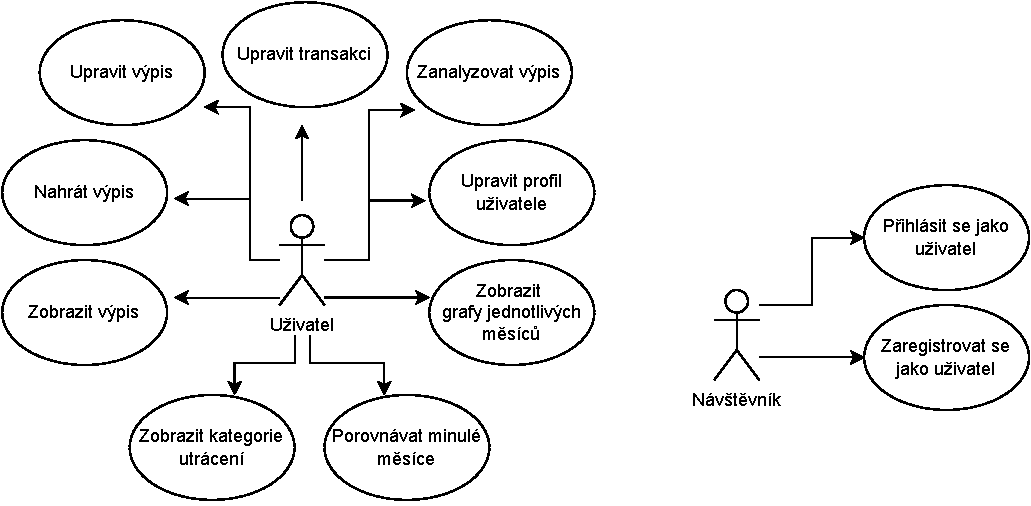
\includegraphics[width=\textwidth]{obrazky-figures/use_case.pdf}
\caption{Diagram případů užití.}
\label{fig;usecase}
\end{figure}

Na obrázku \ref{fig;usecase} můžeme vidět vymodelovaný diagram pro náš navrhovaný systém. Bude mít dva aktéry uživatele a~návštěvníka.
\subsection*{Uživatel}
Uživatelova hlavní akce bude nahrát výpis. Při nahrání výpisu uživatel také může nechat výpis zanalyzovat umělou inteligencí. Od této akce se odvíjí celá řada dalších akcí. Bude mít tyto možnosti: porovnávat jednotlivé měsíce, zobrazit kategorie utrácení, zobrazit daný výpis, upravit jednotlivé transakce, upravit výpis a~upravit profil. 

\subsection*{Návštěvník}
Návštěvník aplikace, kterého potřebujeme rozpoznat a~zajistit mu jednoznačný identifikátor. Tento návštěvník má možnost se zaregistrovat nebo přihlásit se a~tím se přepnout na aktéra uživatel.


\chapter{Návrh}
V~této kapitole bude popsán návrh jednotlivých částí aplikace.

\section{Entity--relationship model}
ER model se v~softwarovém inženýrství používá pro abstraktní a~konceptuální znázornění dat. Znázorňuje, jak bude vypadat naše rozložení dat v~databázi a~jejich vzájemné vztahy~\cite{er_diagram}. 
\begin{figure}[H]
\centering
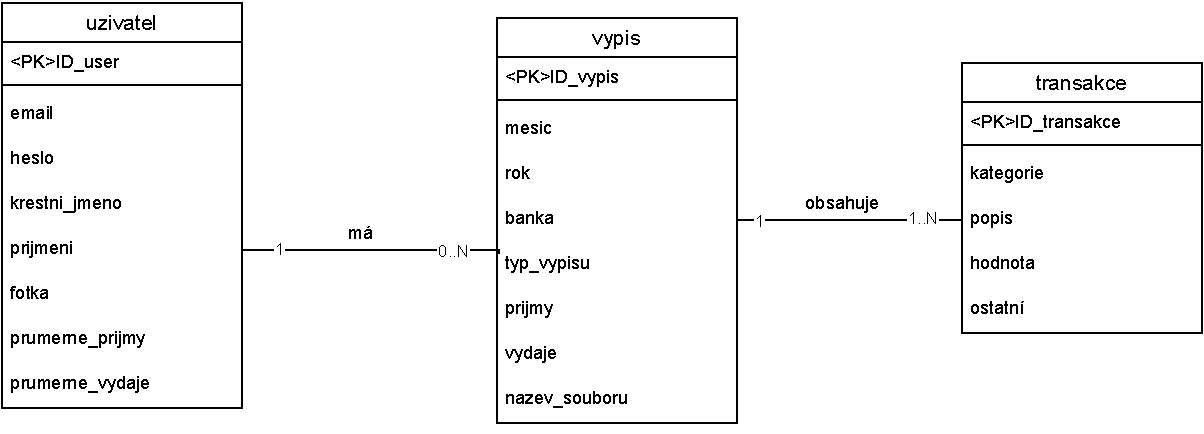
\includegraphics[width=\textwidth]{obrazky-figures/er_diagram.pdf}
\caption{ER diagram.}
\label{fig:erdiagram}
\end{figure}
Náš diagram (obrázek \ref{fig:erdiagram}) bude mít tři entitní množiny -- uživatel, výpis a~transakce.
Uživatel bude mít atributy id, email, heslo, křestní jméno, příjmení, fotka, průměrné příjmy a~průměrné výdaje. Výpis bude mít atributy id, měsíc, rok, banku, typ výpisu, příjmy, výdaje a~název souboru. Transakce bude mít atributy id, kategorie, popis, hodnota a~ostatní.

\section{Návrh uživatelského rozhraní}
Navrhování uživatelského rozhraní (UI design) se v~dnešní digitální době stalo nezbytnou součástí tvorby jakékoliv webové aplikace. Cílem je, aby uživatelé byli schopni snadno ovládat produkt, najít informace a~vykonat požadované úkoly bez zbytečného stresu nebo frustrace. Při mém prvotním navrhováním, jak bude mít aplikace rozmístěné UI prvky jsem zvolil následující rozvržení (obrázek \ref{fig;wireframe}).
\begin{figure}[h]
\centering
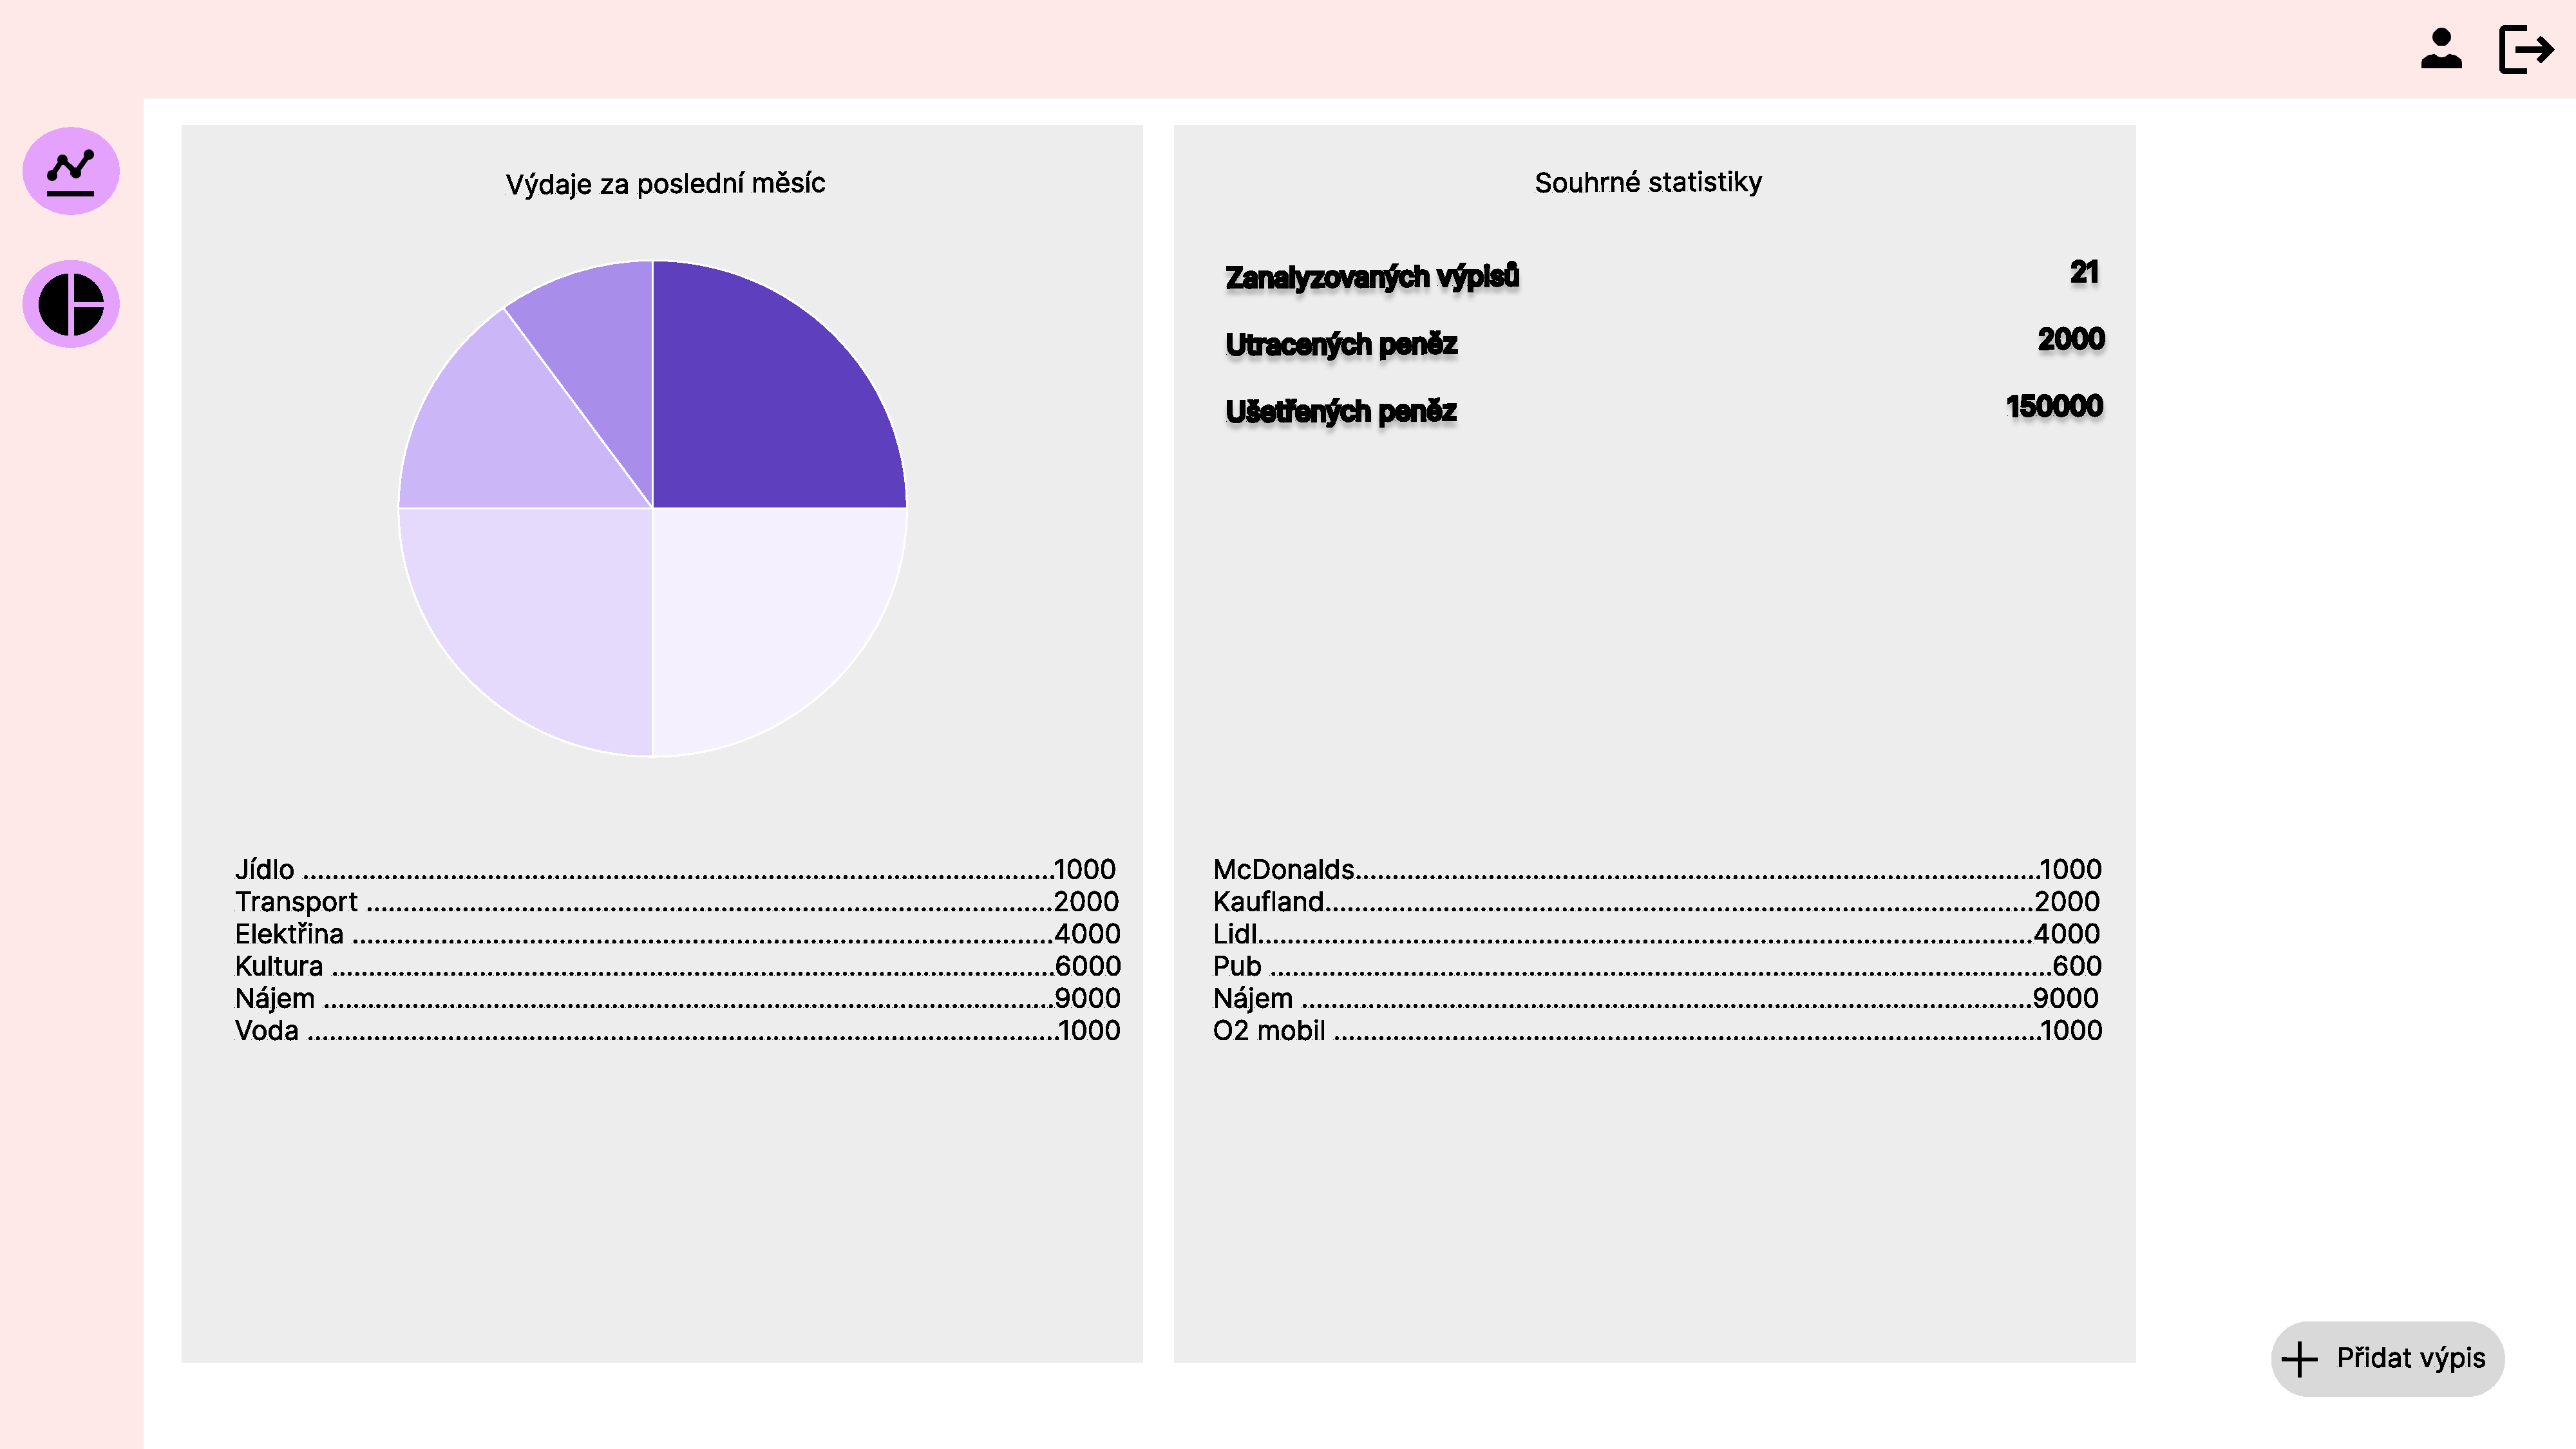
\includegraphics[width=\textwidth]{obrazky-figures/navhrui1.pdf}
\caption{Wireframe domovské obrazovky.}
\label{fig;wireframe}
\end{figure}

Hlavní a~\uv{úvodní} obrazovka, kterou uživatel uvidí první po přihlášení, bude obrazovka s~analýzou výpisu z~posledního měsíce. Nejsignifikantnějším prvkem bude graf s~barevně rozlišenými kategoriemi. Tady si po pravé straně uživatel bude moct prohlížet a~upravovat transakce z~posledního měsíce. Uživatel bude moci najet myší na graf a~zobrazit přesně, ke~které barvě patří jaká kategorie a~kolik v~ní utratil.
Navigace bude mít 5 nejdůležitějších tlačítek Domů, Výpisy, Grafy, Profil a~Odhlášení. Nejdůležitější tlačítko volající o~akci uživatele bude v~levém dolním rohu \texttt{+ Přidat výpis}. Stisknutím tlačítka uživatel nahraje výpis a~následně spustí analýzu transakcí. To vše v~modálním okně, které bude taky znovu použitelné pro editace transakcí nebo výpisů. Kde ve formuláři bude každé políčko jeden atribut z~ER Diagramu (obrázek \ref{fig:erdiagram}) a~půjde jednoduše upravovat.

Na druhé hlavní obrazovce se statistikou může uživatel pozorovat své finance v~dlouhodobém měřítku. Může usoudit, ve které oblasti je potřeba zlepšit své osobní finanční rozhodování. Bude mít k~dispozici souhrnné grafy za posledních několik měsíců, jak lze vidět na obrázku~\ref{fig;wireframe2}.
\begin{figure}[H]
\centering
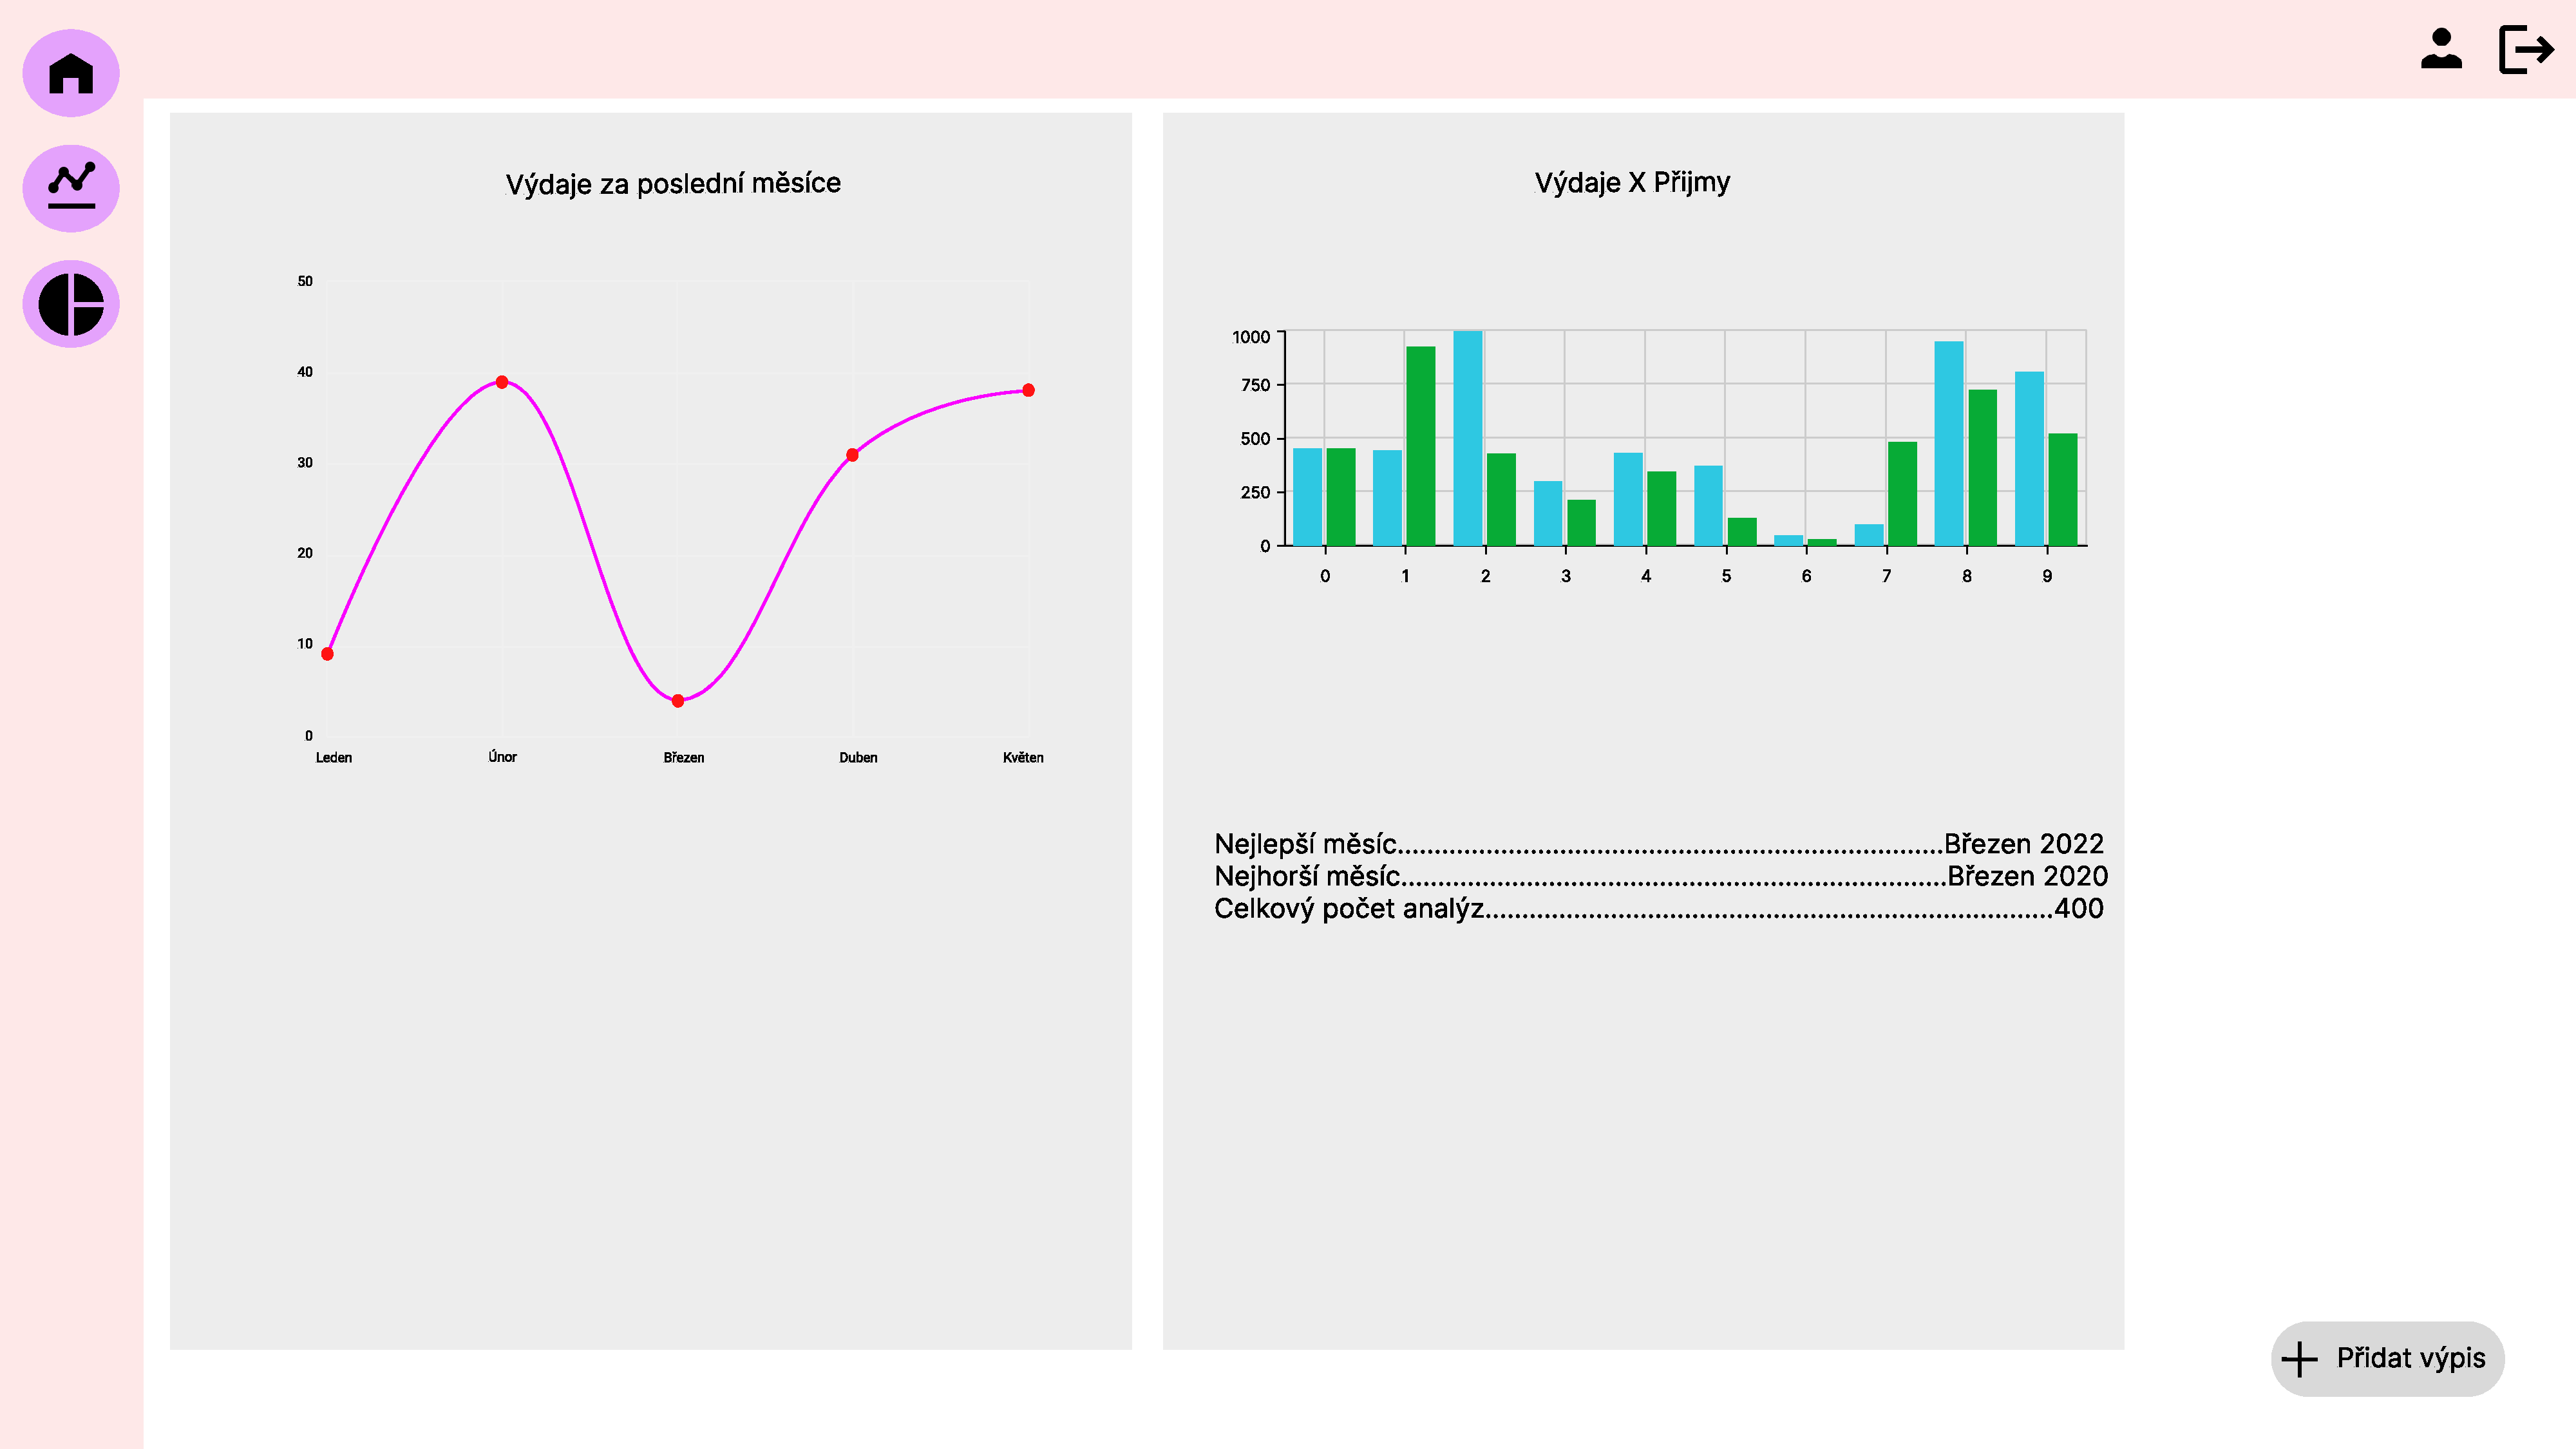
\includegraphics[width=\textwidth]{obrazky-figures/navrhui2.pdf}
\caption{Wireframe obrazovky se statistikou.}
\label{fig;wireframe2}
\end{figure}

\section{Návrh API}
Správný návrh API je klíčovým prvkem při vývoji aplikace a~je nutné se mu věnovat s~dostatečnou pozorností a~pečlivosti. Základní předpoklad pro návrh API je analýza návrhu UI. Zde je potřeba popřemýšlet, jaké datové podklady na které stránce jsou potřeba.
Pro každou entitu je potřeba navrhnout 4 základní HTTP metody. Tyto metody nám poslouží k~vytvoření nové entity, získání dat o~entitě, úpravu entity a~smazání entity. Tento druh endpointů je základ kvalitní aplikace.
Seznam navržených endpointů na serveru, které vyvolávají akci:
 \begin{itemize}
     \item \texttt{GET, POST /user}
     \item \texttt{PUT, DELETE /user/<user\_id>}
     \item \texttt{POST /statement}
     \item \texttt{GET, PUT, DELETE /statement/<statement\_id>}
     \item \texttt{POST /transaction}
     \item \texttt{GET, PUT, DELETE /transaction/<trans\_id>}
     \item \texttt{POST /token}
     \item \texttt{GET /lateststatement}
     \item \texttt{GET /allstatements/}
     \item \texttt{GET /statement/<statement\_id>/transactions}
     \item \texttt{GET /analyze/<statement\_id>}
 \end{itemize}
Pojmenování těchto CRUD endpointů se řídí pravidly REST API. To znamená, že~endpointy~(transakce, výpis) se pojmenovávají dle tohoto klíče. GET, PUT a~DELETE \break \texttt{/<jméno\_entity>/<identifikační\_číslo>} a~POST \texttt{/<jméno\_entity>/}. Na výpisu \ref{lst:httpget} lze vidět jak požadavek a~odpověď vypadají.
\begin{lstlisting}[breaklines=true,caption={Příklad požadavku \texttt{GET /statement/84}.},label={lst:httpget}]
GET http://127.0.0.1:5000/statement/84
{
    "bank": "Komercka",
    "filename": "kb_november.csv",
    "id": 84,
    "income": 40462,
    "month": 12,
    "spending": 40090,
    "type": "Checkings",
    "year": 2022
}
\end{lstlisting}

Pojmenování endopointu pro entitu uživatel je odlišné, protože díky JWT autentizačnímu tokenu v~hlavičce požadavku dokážeme rozeznat uživatele bez potřeby identifikačního čísla umístěného na konci endpointu. Z~tohoto důvodu bude pro metody GET a~POST endpoint pojmenován \texttt{/uzivatel/} a~pro PUT a~DELETE bude pojmenován\break \texttt{/uzivatel/<identifikační\_číslo>}.

Další endpoint \texttt{/token} slouží na získání autentizačního tokenu JWT, který následně vloží klient do hlavičky HTTP požadavku. Tento endpoint je důležitý pro přihlášení a~autentizaci uživatele.

Následuje skupina endpointů \texttt{/lateststatement}, který vrací výpis z~posledního měsíce a~\texttt{/allstatements}, který vrací všechny uživatelovi výpisy, zjištění uživatele lze znova poznat pomocí autentizační hlavičky.
Kombinovaný endpoint dvou entit \break \texttt{/statement/<statement\_id>/transactions} vrací data o~všech transakcích, které daný výpis obsahuje.

Poslední endpoint \texttt{/analyze} nevrací nic, pouze provede na daném výpisu kategorizaci transakcí a~přidá transakce do databáze.


\chapter{Implementace}
V~následující kapitole budou popsány implementační detaily serveru a~klienta.

\section{Implementace serveru}
Server běží na webovém frameworku Flask. Server je rozdělen do několika podsouborů. Hlavní soubor, který tvoří jádro celé aplikace je pojmenovaný \texttt{server.py}, zde běží celé API, a~v~dalších třech souborech běží model umělé inteligence (\texttt{model.py}), extrakce dat z~výpisu (\texttt{template\_analyze.py}) a~kategorizace výpisů 
 bez AI (\texttt{static\_analyze.py}).
 
\subsection{Implementace API}
Flask nabízí jednoduché a~minimalistické vytvoření API. K~rozběhání serveru stačí inicializovat Flask do proměnné \texttt{app} a~následně ji spustit. Pro napojení na databázi potřebujeme Python knihovnu SQLAlchemy\footnote{\url{https://www.sqlalchemy.org/}}. Tato knihovna nám umožní pracovat s~databází v~prostředí Python a~zpřístupní nám možnost vymodelovat databázi. Podobně jako Flask i~SQLAlchemy se musí inicializovat a~následně pracovat pod proměnou \texttt{db}. Pro každou entitu z~ER diagramu vytvoříme třídu s~definicí, jaké atributy má daná třída mít v~databázi. Pro získávání dat z~databáze pomocí dotazů je vytvořena speciální třída se schématem, který je typově stejný jako související třída pro databázový model. Tato třída je z~knihovny Marshmallow\footnote{\url{https://flask-marshmallow.readthedocs.io/en/latest/}} slouží pro deserializaci databázového objektu. To znamená, že díky převodu na schéma je možné rovnou posílat data v~JSON formátu.


Každý endpoint se definuje ve webovém frameworku Flask pomocí \break \texttt{@app.route('/cesta', methods=["POST"])}, zde si může nastavit požadovanou URI a~povolené HTTP metody.

V~metodě GET pomocí knihovny SQLAlchemy je vytvořen hledací dotaz do databáze \break (např. \texttt{User.query.filter\_by(id=user\_id).first()}). Tento příklad vrací objekt User s~hledaným identifikátorem, díky převodu na schéma můžou být informace o~objektu poslány zpět na klienta.

V~metodě POST se odeslaná data z~klienta na serveru přijmou ve formátu JSON. Na serveru se uloží do proměnné pomocí \texttt{request.json} všechny informace z~těla HTTP zprávy. Tato proměnná použije funkci \texttt{data.get('klíč')}. Klíč definuje, která hodnota z~JSON formátu bude vybrána a~uložena. Poté se všechny hodnoty uloží do třídy s~příslušným názvem a~pomocí \texttt{db.session.add('třída')} a~\texttt{db.commit()} se objekt vkládá do databáze.

Metoda PUT operuje podobně jako metoda POST s~tím rozdílem, že se první pokusí najít objekt, který má upravovat v~databázi.

Metoda DELETE pouze vyhledá v~databázi objekt a~příkazem \break \texttt{db.session.delete(objekt)} smaže objekt.
Po každé úpravě databáze musí být volána funkce \texttt{db.session.commit()} pro perzistentní stav databáze.


\subsection{Extrakce dat z~šablony}
Jak jsem již formuloval v~kapitole \ref{chap:formaty}, každá banka má rozdílné výpisy transakcí. Proto je potřeba pro každou banku vytvořit vlastní funkci k~extrakci dat.
\subsubsection{AirBank}
AirBank používá formát CSV v~kódování WIN-1250. Funkce \texttt{Airbank\_analyze()} otevře soubor pro čtení a~pomocí knihovny pro čtení CSV souboru otevře soubor a~hledá požadované sloupečky v~souboru: \uv{Název protistrany} a \uv{Částka v~měně účtu} tyto dvě informace nám stačí pro vytvoření objektu Transakce a~spuštění automatické klasifikace transakce.

\subsubsection{Fio}
Fio nabízí své výpisy v~CSV formátu. Postup je podobný jako u~AirBank. Otevřeme CSV soubor a~hledáme sloupečky v~souboru, které obsahují podrobné informace o~transakci (\uv{Název obchodníka} popřípadě \uv{Poznámka}, \uv{Zaúčtovaná částka}).

\subsubsection{Československá obchodní banka}
ČSOB nabízí výpisy ve formátu XML i~s~jejich detailně popsanou dokumentací\footnote{\url{https://www.csob.cz/portal/documents/10710/1927786/ceb-vypisy-format-xml.pdf}}. Pomocí knihovny XML pro načtení stromové struktury do proměnné postupně procházíme strukturou a~hledáme položky s~tagem \uv{Ntry} pro zjištění, že se jedná o~záznam o~transakci. V~transakci hledáme \uv{Amt} pro zjištění částky a~dále zjišťujeme pomocí tagu \uv{CdtDbtInd} zda je platba kladná (\uv{CRDT}) nebo záporná (\uv{DBIT}). A~po dalším zanoření hledáme \uv{NtryDtls} neboli detail transakce. A~pro samotný popis transakce se musíme zanořit ještě o~dvě úrovně níž na položku \uv{Ustrd}, ze které musíme odstranit lokaci a~částku pro další kategorizaci.

\subsubsection{Moneta}
Moneta taktéž nabízí výpisy ve formátu XML a~poskytuje jejich detailně popsanou strukturu\footnote{\url{https://www.moneta.cz/documents/20143/11740743/mmb-ib-struktura-vypisu-xml.zip}}. Moneta má na rozdíl od ČSOB jednodušší stromovou strukturu a~hledáme pouze elementy s~tagem \uv{transaction}, kde pak hledáme atributy s~názvem \uv{amount} pro částku a~pro popis transakce se zanoříme do \uv{trn-messages} a~následně do \uv{trn-message}. V~tomto bodě zanoření byl nalezen popis transakce a~můžeme spustit automatickou kategorizaci a~uložit objekt do databáze.

\subsubsection{Komerční banka}
Komerční banka poskytuje své výpisy ve formátu CSV. Na rozdíl od ostatních bank přidává do svých výpisů nadstandardně velkou hlavičku, kterou je nutné odstranit. Po analýze několika výpisů od různých lidí se mi potvrdilo, že nejlepší cestou bude otevřít soubor odstranit z~něj prvních 17 řádků, uložit a~až potom ho načíst knihovnou pro čtení CSV. Dále procházíme soubor a~hledáme sloupečky \uv{AV pole 1} a~pole \uv{Částka}. Tato data nám stačí pro přidání objektu Transakce do databáze. Zkusíme spustit automatickou detekci kategorie a~transakci uložíme.

\subsubsection{UniCredit bank}
UniCredit banka poskytuje výpisy ve formátu CSV. Tyto výpisy podobně jako výpisy z~Komerční banky obsahují hlavičku. Proto je nutné  odstranit z~nich prvních 5 řádků, uložit soubor a~až potom jej načíst knihovnou pro čtení CSV. Dále procházíme soubor a~hledáme sloupce \uv{Částka} a~\uv{Příjemce}. Následně spustíme automatické řazení transakcí a~uložíme transakce do databáze.


\subsubsection{Budoucí přidání dalších bank}
\label{chap:addbank}
Budoucí rozvoj aplikace a~přidávání všech českých a~světových bankovních společností je vítaným rozšířením. Největším problémem s~přidáním nové banky je získání dostatečného množství vzorků výpisů z~banky. Bankovní společnosti nebyly nejochotnější v~komunikaci s~poskytnutí testovacích výpisů. Po dostatečné analýze je potřeba pouze vytvořit novou funkci v~souboru \texttt{template\_analyze.py}. Je potřeba vytvořit funkci, která přečte celý soubor, najde příslušné položky ve výpisy (částku, popis transakce), provede kategorizací a~přidá transakci do databáze.


\section{Implementace klienta} 

Klient běží na webovém frameworku React. Celkové rozložení implementace je složeno z~menších komponent, které dohromady tvoří celé stránky v~aplikaci.
\subsection{Použité balíčky}
React má obrovskou komunitní základnu a~proto je k~dispozici mnoho balíčků, které nám s~ním umožní lépe pracovat. V~následujících kapitolách popíši jen ty nejzajímavější.
\subsubsection{Material UI}
Material UI\footnote{\url{https://mui.com/}} je open source knihovna uživatelského rozhraní pro React framework, která poskytuje předdefinované komponenty a~stylizaci v~souladu s~designovým jazykem Material Design od Google\footnote{\url{https://m1.material.io/}}. Material UI přináší rozsáhlou nabídku přizpůsobitelných komponent, zahrnujících tlačítka, formulářová pole, ikony, nabídky a~další prvky, které lze snadno implementovat pro vytvoření moderního, jednotného a~esteticky příjemného uživatelského rozhraní. Tato knihovna nabízí možnosti vysokého stupně flexibility a~přizpůsobení, což umožňuje vývojářům snadno upravit vzhled a~funkčnost komponent, které zrovna vývojář potřebuje. Knihovna disponuje skvěle zpracovanou dokumentací, což představuje jednu z~hlavních faktorů, proč jsem se rozhodl ji využít.

\subsubsection{Axios}
Axios\footnote{\url{https://www.npmjs.com/package/axios}} je Javascriptová knihovna, která umožňuje vytváření HTTP požadavků v~prostředích s~použitím React frameworku. Tato knihovna poskytuje vývojářům širokou knihovnu funkcí pro získávání a~odesílání dat mezi klientem a~serverem. 

\subsubsection{Toastify}
Toastify\footnote{\url{https://fkhadra.github.io/react-toastify/introduction}} je knihovna pro React, která umožňuje uživatele upozorňovat (tzv. toast zprávou) na různé změny a~události. Tyto upozornění se většinou nachází v~jednom ze čtyř rohů obrazovky.

\subsubsection{Recharts}
Knihovna Recharts\footnote{\url{https://recharts.org/en-US/}} je open--source a~slouží k~vytváření interaktivních grafů. Knihovna nabízí mnoho různých typů grafů, jako jsou liniové grafy, sloupcové grafy, koláčové grafy, časové osy a~další. Stala se velmi populární hlavně z~důvodů obrovské možnosti přizpůsobení grafů (např. barvy, šířku čar, styl os atd.).

\subsection{Komponenty}
Dle návrhu je práce rozdělena na několik menších stránek. Každá stránka se skládá ze samostatné komponenty nebo z~více komponent. 
Ve složce \texttt{src/componenets} je pro každou komponentu vyhrazen samostatný soubor.
Zajímavější komponenty jsem se snažil rozebrat v~následujících kapitolách.

\subsubsection{App.js}

Funkce \texttt{App} definuje a~inicializuje základní strukturu aplikace. Používá se zde komponenta BrowserRouter, která poskytuje routing pro aplikaci, a~inicializuje komponentu ToastContainer, která bude zobrazovat zprávy pro uživatele v~rámci celého prostředí aplikace. Routing pro aplikaci znamená, že vytvoří cesty pro jednotlivé stránky, aby měla každá stránka svou URL.
\subsubsection{UseToken.js}

Tato komponenta pracuje hlavně s~JWT tokenem. Obsahuje tři funkce \texttt{getToken}, \texttt{saveToken} a~\texttt{removeToken}. Funkce \texttt{saveToken} uloží JWT token do Local Storage a~pokud bude klient posílat další požadavky bude token jednoduše získatelný. Funkce \texttt{getToken} dokáže získat uložený JWT token z~Local Storage a~znovu ho použít při dalším HTTP požadavku. Funkce \texttt{removeToken} odstraní z~Local Storage token a~tím se uživatel nemá jak autentizovat při dalším HTTP požadavku.
\subsubsection{Login.js}

Je jedna z~nejdůležitějších komponent aplikace, zde se uživatel autentizuje do aplikace. Uživatelovi se zobrazí formulář pro zadání svých inicializačních údajů. Pomocí zadání své emailové adresy a~hesla, a~následným kliknutím na tlačítko \texttt{Sign in}, odešle klient pomocí Axios knihovny HTTP požadavek, který vrátí autentizační token. Pokud server vrátí úspěšnou odpověď na požadavek, přesměruje se klient na stránku \texttt{Home.js}. V~případě, že autentizace selže, dojde k~resetování polí pro zadání údajů a~zobrazení zprávy o~neúspěchu.

\subsubsection{Home.js}
Domovská obrazovka, jak z~návrhu vyplývá, je první obrazovka se kterou se setká uživatel. Vnitřní logika volá endpoint pro získání dat z~posledního výpisu a~následuje endpoint na všechny transakce daného výpisu. Tato data dále posílá jako argumenty do dalších komponent. Na obrázku \ref{fig:homescreen} lze vidět rozdělení na 4 komponenty -- Navigační lišta (\texttt{NavBar}), Nahrávání výpisu (\texttt{Upload}), Výpis transakcí (\texttt{Transaction}) a~Výsečový diagram (\texttt{Graph}). 

\begin{figure}[ht]
    \centering
    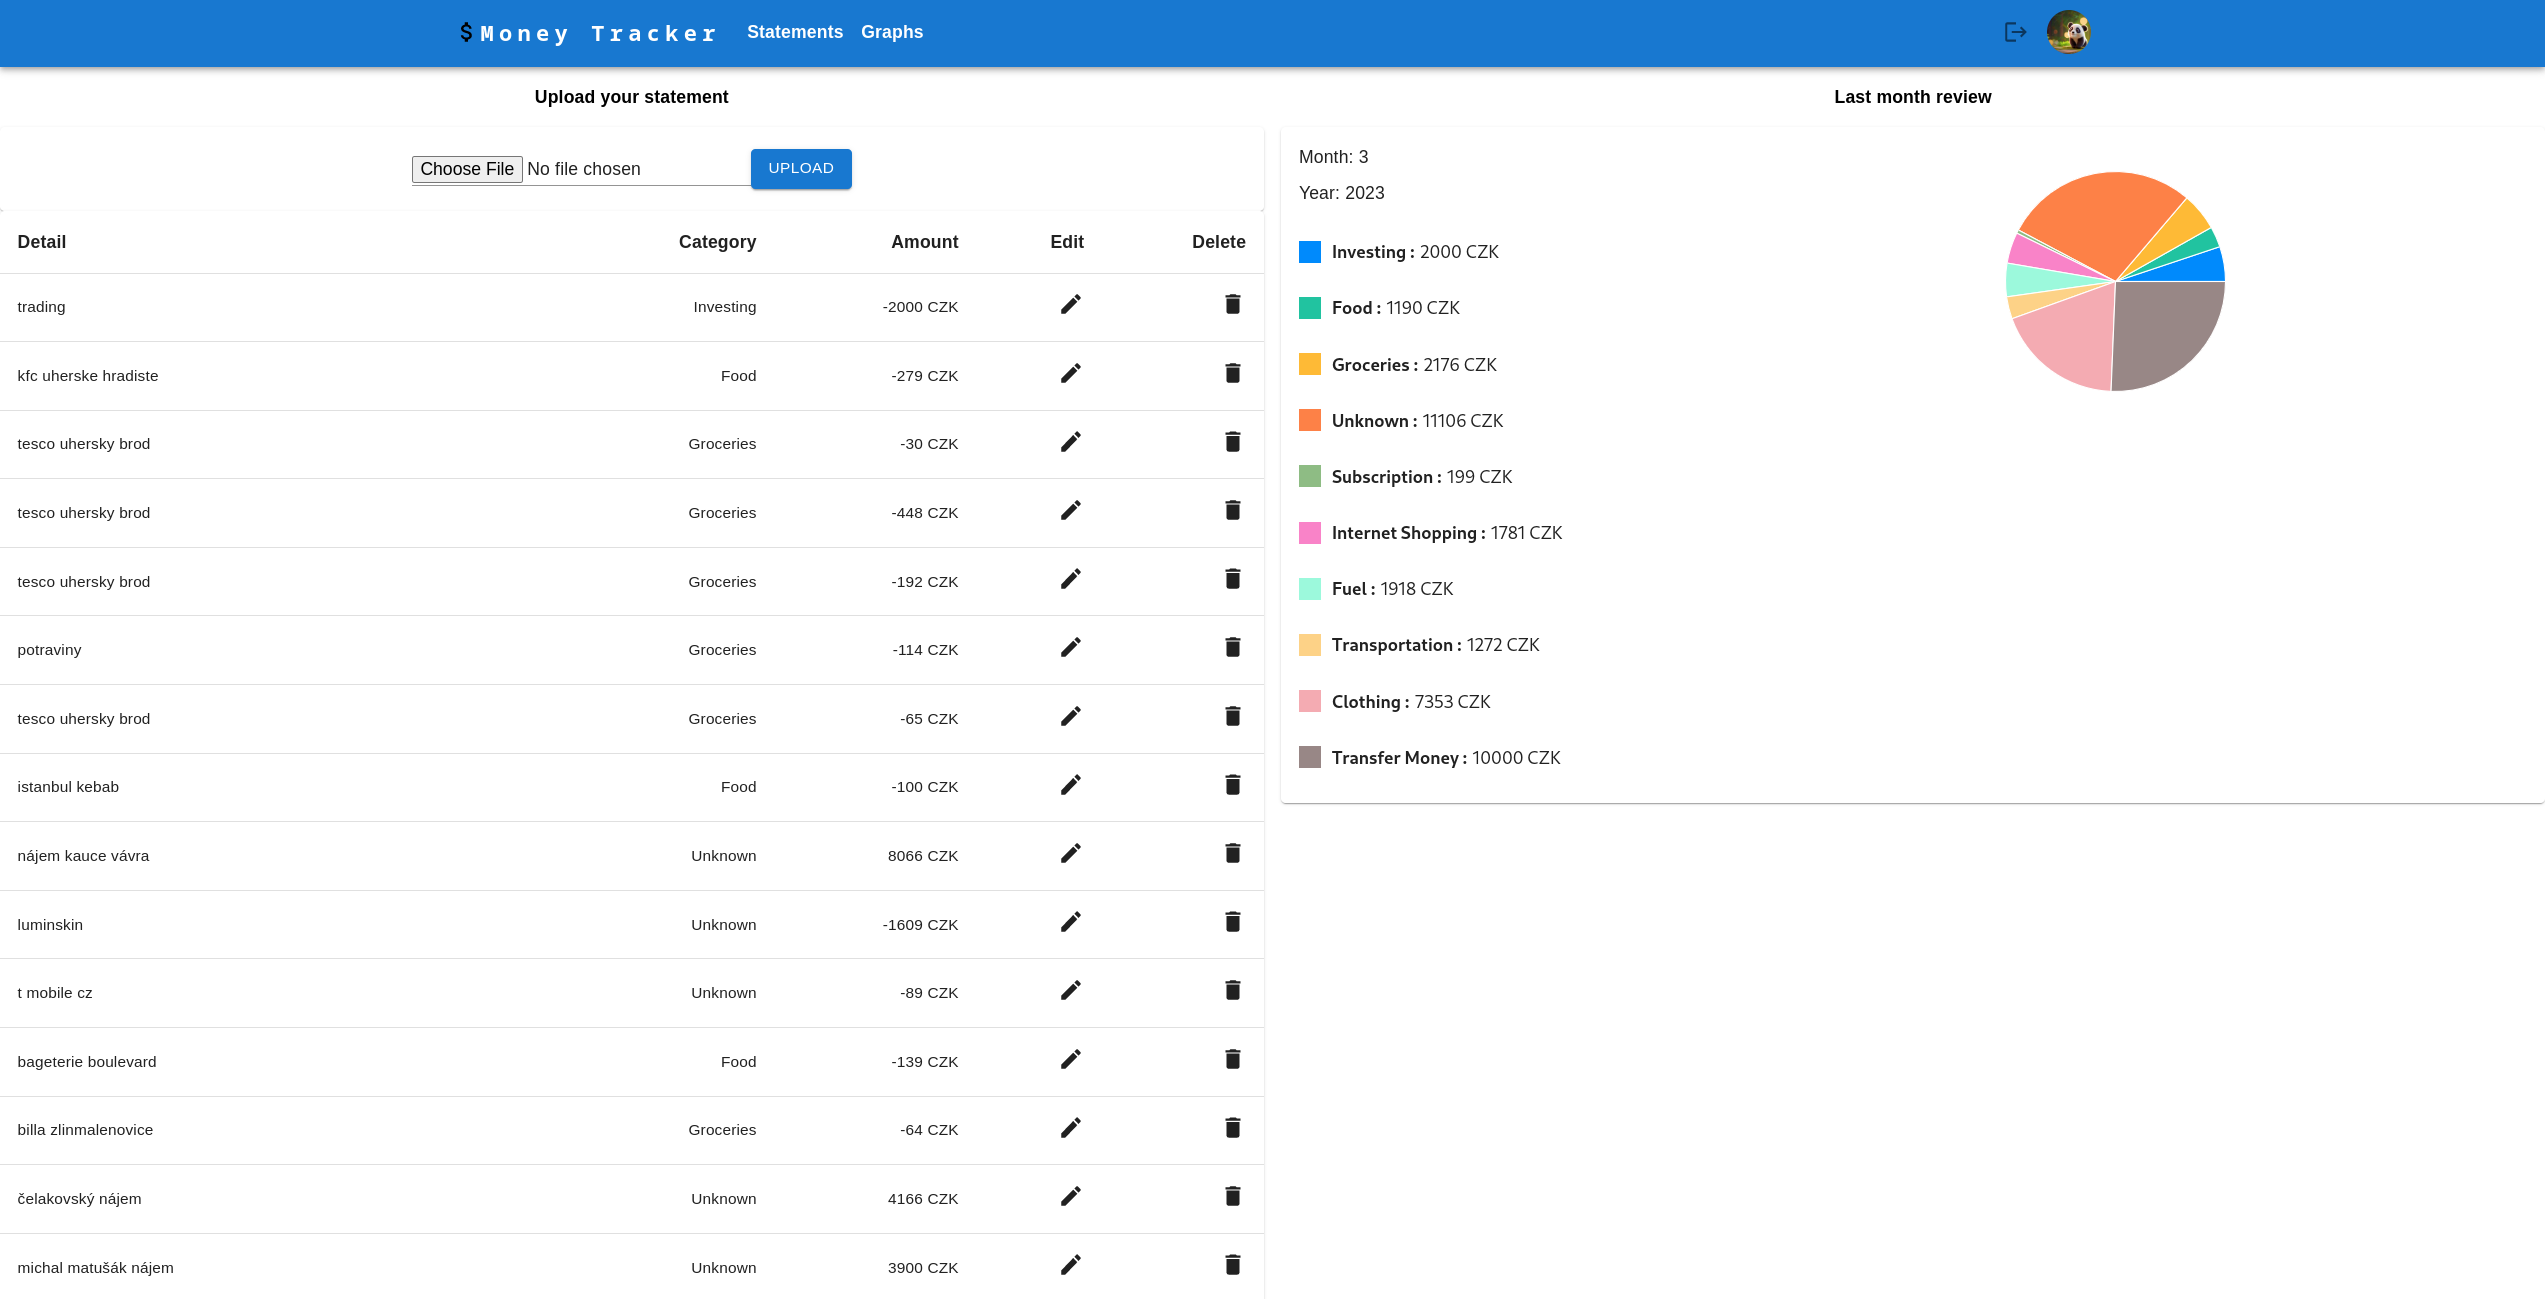
\includegraphics[width=\textwidth]{obrazky-figures/moneyhome.png}
    \caption{Domovská obrazovka aplikace.}
    \label{fig:homescreen}
\end{figure}

\subsubsection{Transaction.js}
Transactions zobrazuje tabulku všech transakcí, které jsou předány jako argument. Pomocí mapovací funkce \texttt{transaction.map()} se tabulka rozšíří nebo zmenší na základě poskytnutých dat. Tabulka zobrazí všechny důležité parametry entity Transakce. Uživatel může díky ikonám rychle upravovat jednotlivé transakce v~modální okně nebo je rovnou smazat.

\subsubsection{Graph.js}
Komponenta obsahuje funkci \texttt{countAmountByCategory}, která vezme data z~transakcí a~spočítá sumu za jednotlivé kategorie, které se nachází v~datech. Funkce data připraví do formátu \texttt{kategorie:částka}, aby je mohla knihovna \texttt{Recharts} použít. Tato data se potom zobrazí v~barevném grafu. 
Tato komponenta se zobrazuje Graf na základě dat transakcí, které komponenta dostane jako argument. 

\subsubsection{Upload.js}
Tato komponenta dovolí uživatelovi nahrát soubor. Po kliknutí na tlačítko \texttt{Upload} se soubor pomocí POST požadavku odešle na server a~pokud přijde kladná odpověď, klient si uloží identifikační číslo výpisu. Uživatelovi se zobrazí modální okno s~požadavkem na vyplnění dodatečných údajů, které se pomocí PUT požadavku pošlou zpět na serveru a~začne analýza transakcí. Dokud není hotova uživatel vidí načítací kolečko, jakmile klient přijme kladnou odpověď serveru přesměruje klienta na detail výpisu.
\begin{figure}[H]
    \centering
    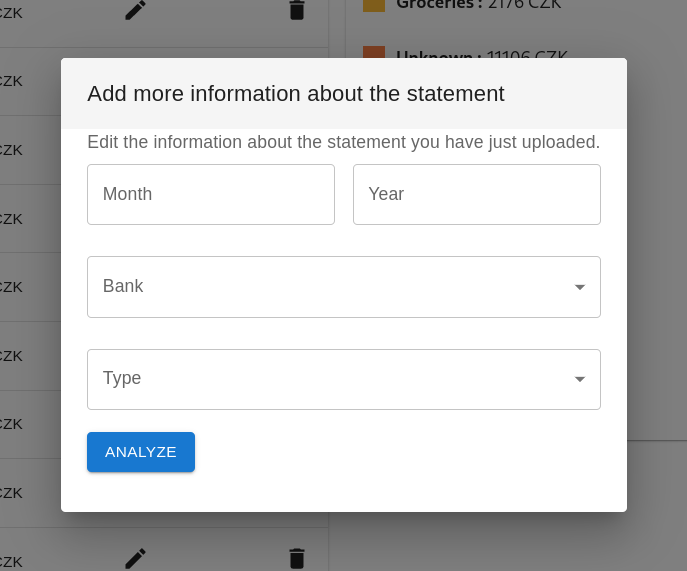
\includegraphics[width=7cm]{obrazky-figures/moneymodalwindow.png}
    \caption{Modální okno pro doplnění informací o~výpisu.}
    \label{fig:statements}
\end{figure}


\subsubsection{Graphs.js}
Stránka s~přehlednými grafy je schovaná v~komponentě \texttt{Graphs.js}. Zde se kromě Navigační lišty nachází dva grafy, jeden zobrazující porovnání příjmů a~výdajů v~průběhů měsíců v~daném roce. Na druhém grafu se zobrazuje křivka výdajů. Pomocí komponenty YearCalendar, která při změně vybraného roku vždy pošle nový požadavek na server a~znovu načte dotčené komponenty, může uživatel měnit časové rozmezí pro data v~grafu.
\begin{figure}[H]
    \centering
    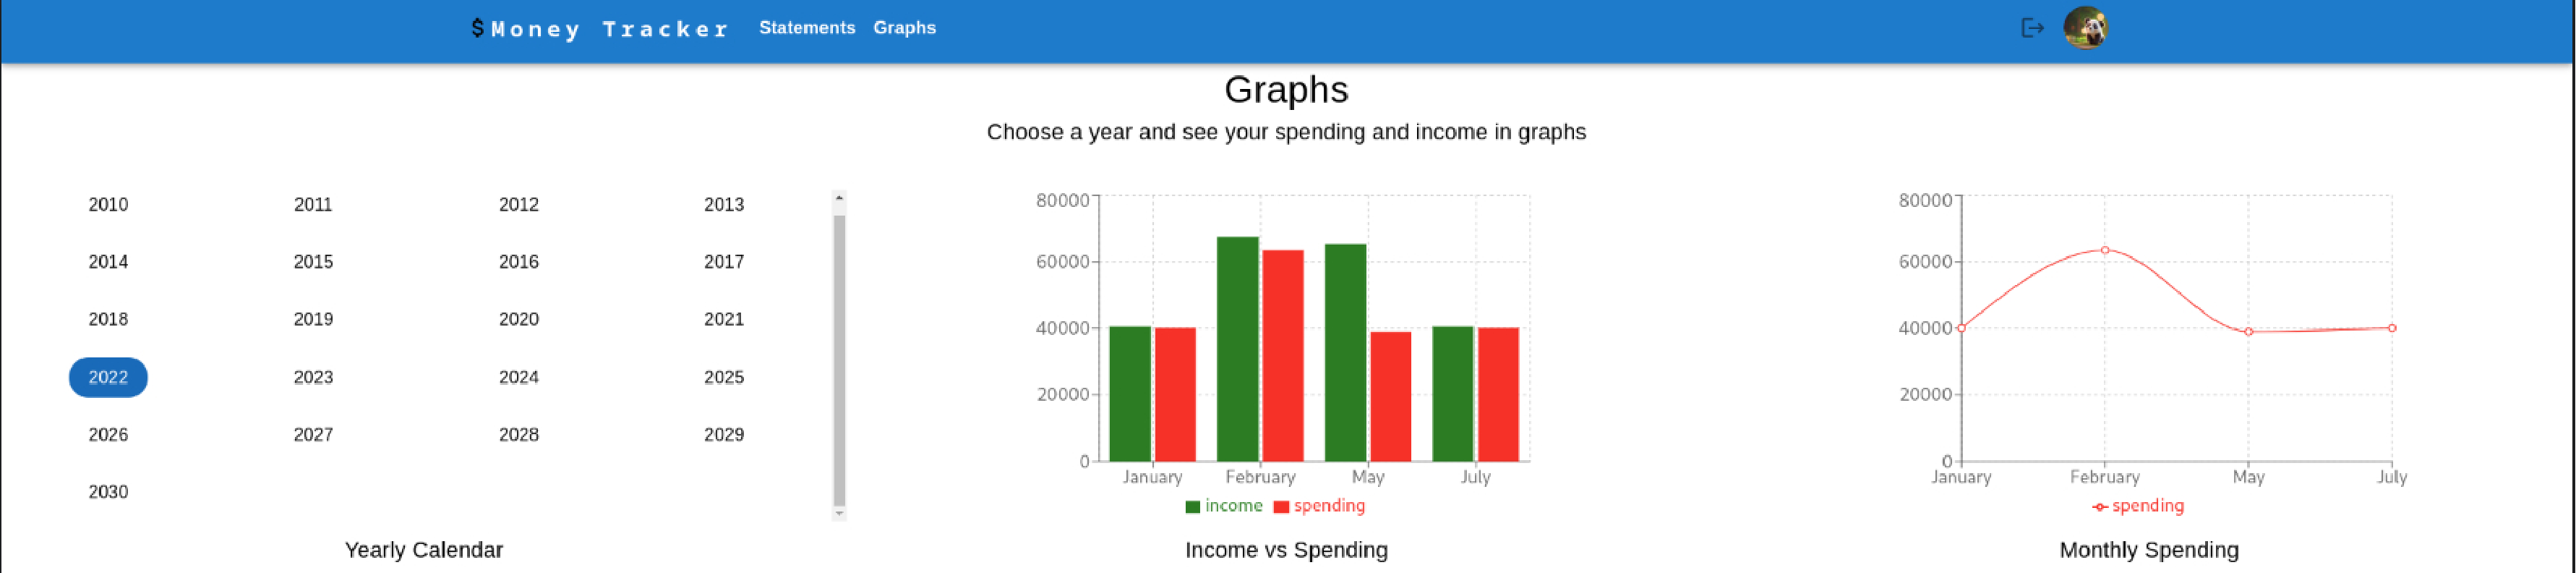
\includegraphics[width=\textwidth]{obrazky-figures/moneygraphs.pdf}
    \caption{Obrazovka pro sledování výdajů v~čase.}
    \label{fig:graphs}
\end{figure}


\subsubsection{Profile.js}
Tato stránka umožní uživateli upravit svůj profil, pomocí komponenty TextField z~Material UI. Předtím než uživatel bude moct data upravovat je zavolán endpoint \texttt{GET /user}, ten nám zajistí nahrání dat do formulářových polí. Uživatel může upravovovat všechny položky, které obsahuje entita Uživatel. Tlačítko vyvolá akci \texttt{SubmitPut}, tato akce zkontroluje zda heslo bylo upraveno a~zkontroluje zda bylo zadáno dvakrát. Tato kontrola je důležitá z~důvodu velice častých chyb, které může uživatel udělat. Následně odešle požadavek\break \texttt{PUT /user/<identifikační\_číslo>} a~klient zobrazí dle odpovědi serveru kladnou nebo zápornou zprávu. Na obrázku \ref{fig:profile} lze vidět úpravu jednoho z~uživatelů.

\begin{figure}[H]
    \centering
    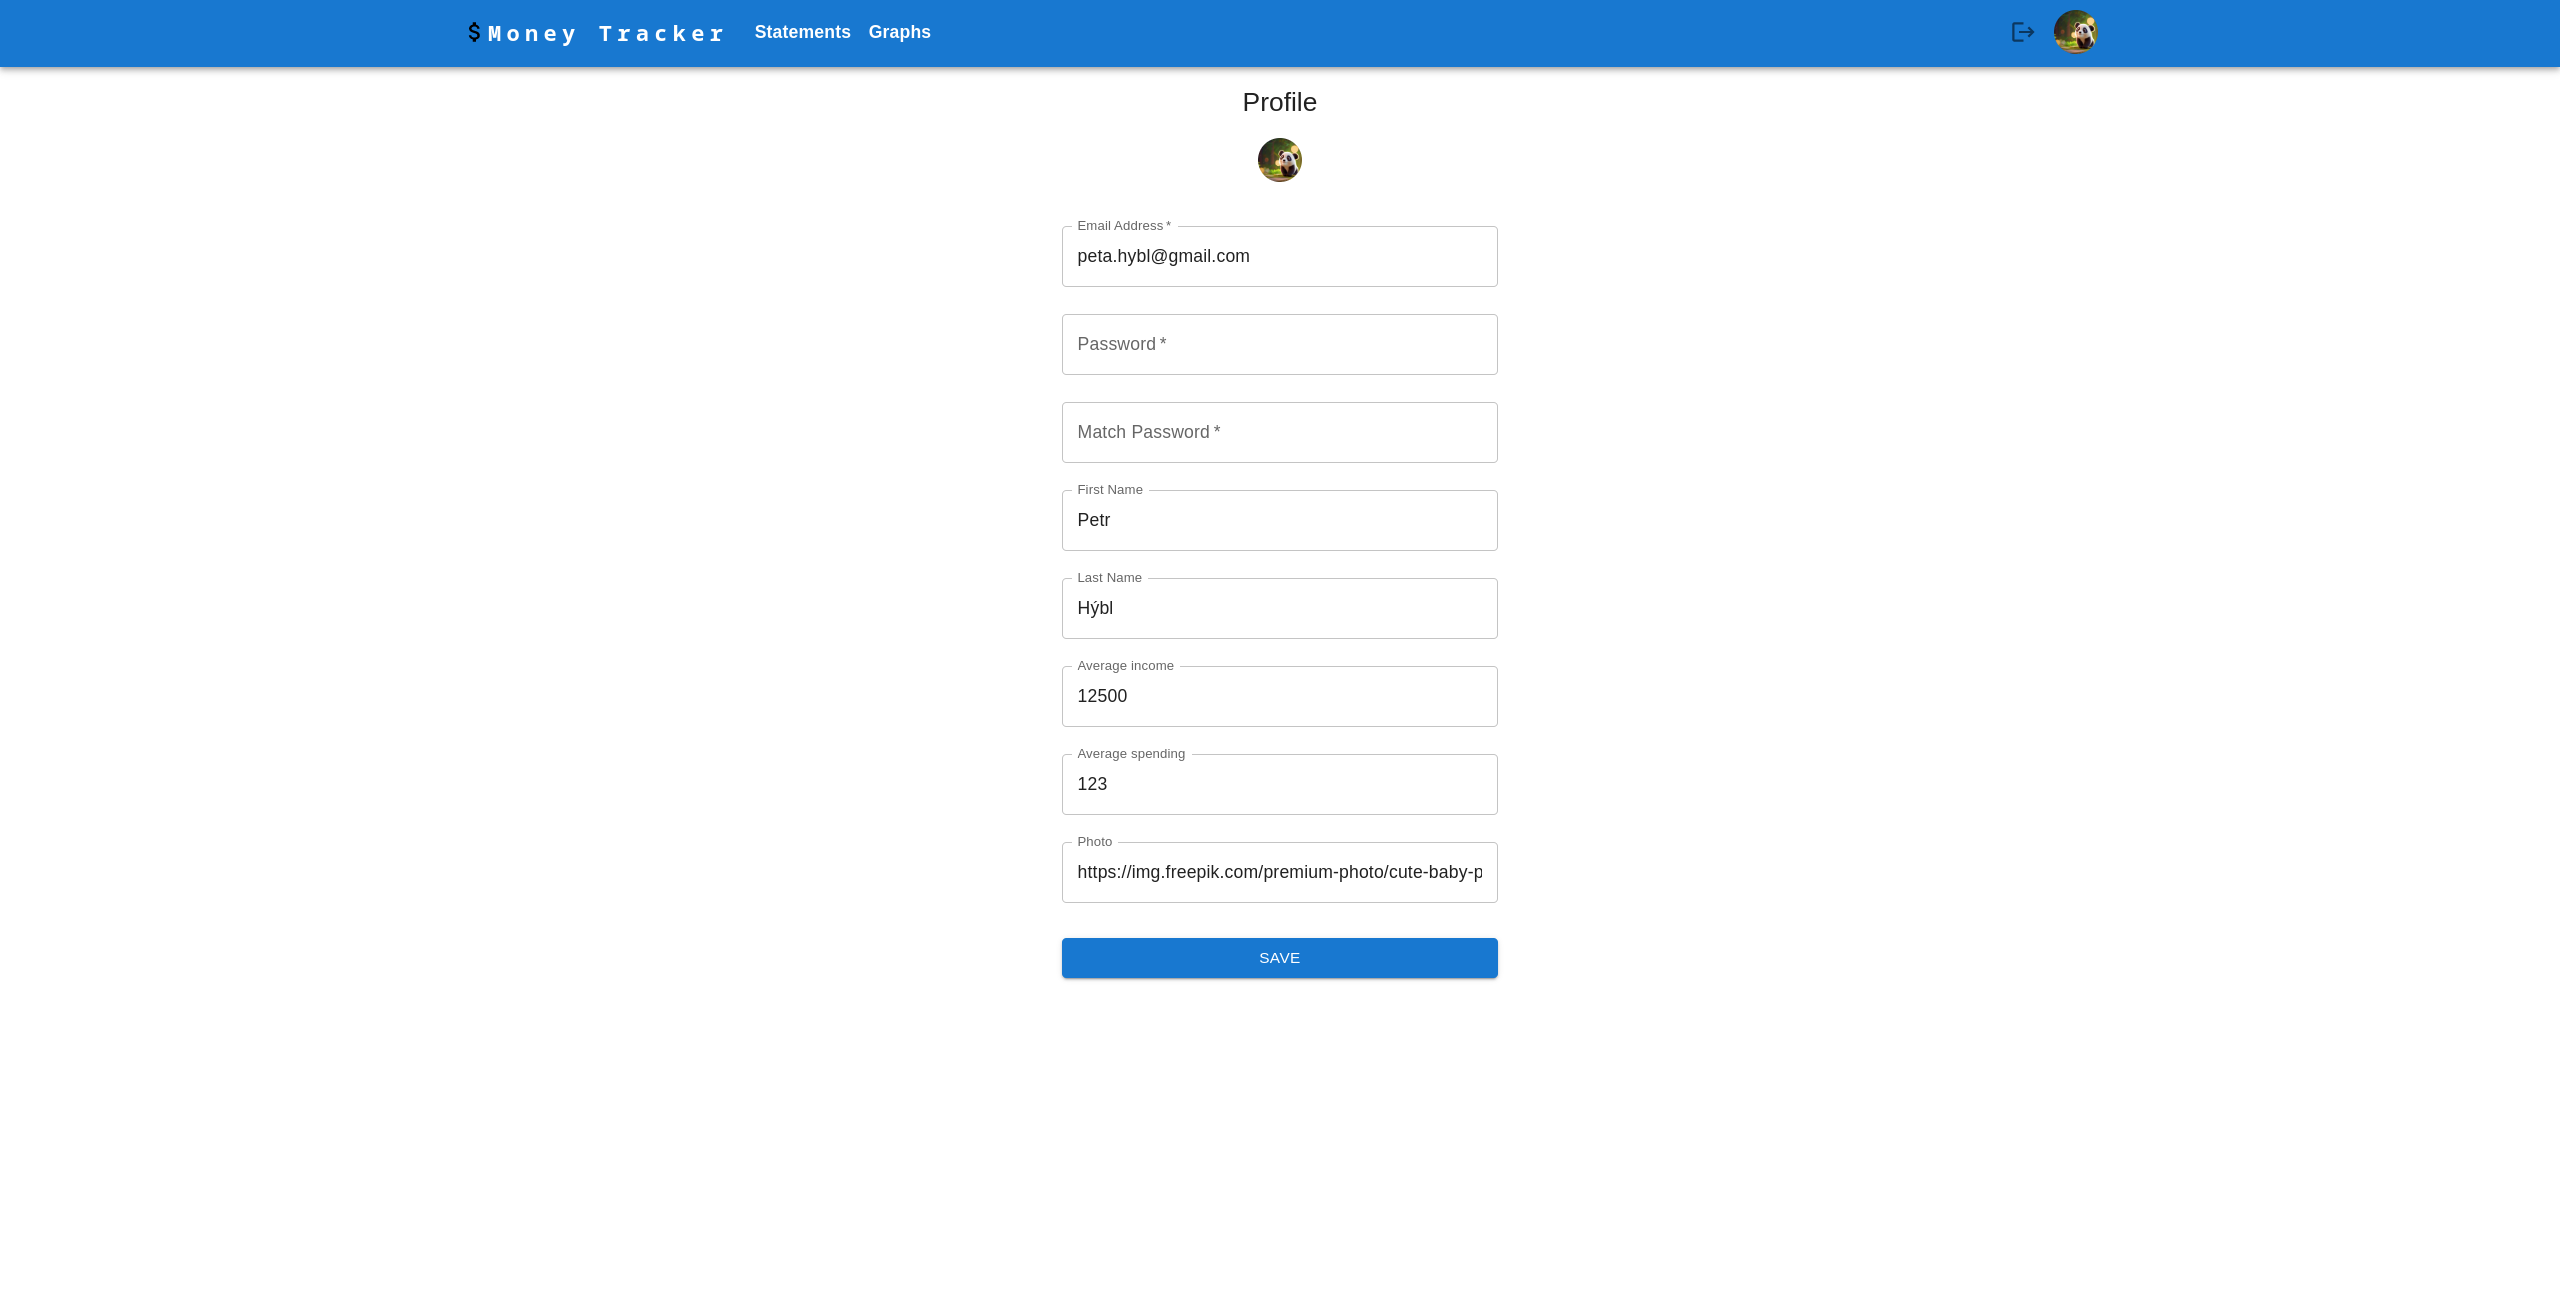
\includegraphics[width=\textwidth]{obrazky-figures/moneyprofile.png}
    \caption{Obrazovka pro úpravu uživatele.}
    \label{fig:profile}
\end{figure}

\subsubsection{Statements.js}
Uživatel využije tuto komponentu při zobrazování detailu jednoho určitého výpisu. Komponenta načítá data z~endpointu \texttt{/allstatements/}. Po načtení dat jsou zobrazeny v~tabulce, kde každý řádek odpovídá jednomu bankovnímu výpisu a~zahrnuje informace o~měsíci, roce, bance, typu, příjmu a~výdajích. Kliknutím na tlačítko \texttt{Edit} v~řádku daného bankovního výpisu se otevře dialogové okno s~editačním formulářem, který umožňuje změnit údaje v~daném záznamu. Po změně údajů je možné uložit změny na server pomocí tlačítka, které volá na endpoint \texttt{/statement/<identifikační\_číslo>}.




\chapter{Automatická klasifikace transakcí}
Různé banky nabízí různé formáty výpisů, jak jsem již uvedl v~kapitole \ref{chap:formaty}, a~tak pokud je chceme automaticky kategorizovat, je potřeba extrahovat stejná data z~každého výpisu. Nejdůležitějším parametrem je \uv{Popis transakce} (v~každé bankovní společnosti se tento parametr nazývá jinak např. \uv{Zpráva} nebo \uv{AV Pole 1} atd.). Tento parametr poskytuje mnoho užitečných informací, jako je jméno příjemce nebo název společnosti, který lze využít pro další kategorizaci.

\section{Python knihovny}
Automatická kategorizace pomocí umělé inteligence se neobejde bez doplňujících knihoven. V~následujících kapitolách si některé upřesníme k~čemu budou použity.
\subsection{PyTorch}
PyTorch\footnote{\url{https://pytorch.org/}} je framework pro strojové učení, který byl vyvinut především pro výzkum v~oblasti umělé inteligence a~neuronových sítí. Tato knihovna umožňuje vývojářům vytvářet a~trénovat složité neuronové sítě. Tuto knihovnu jsem si zvolil pro její vysokou flexibilitu a~efektivitu. PyTorch je základem pro další knihovny, které dále budu používat.

\subsection{Sentence Transformer}
Sentence Transformer je nadstavba pro framework PyTorch, která dokáže vytvořit reprezentaci vět, textů a~obrázků. Tento nástroj lze použít pro výpočet vektorů vět pro více než 100 jazyků, a~poté pomocí kosinové podobnosti porovnat věty s~podobným významem. Tato funkce je užitečná pro sémantické hledání podobností, sémantické vyhledávání nebo hledání parafrází. Nabízí spoustu předtrénovaných modelů a~pro moji práci zvolíme model \textsc{paraphrase-multilingual-mpnet-base-v2}, který byl vytrénován na vícejazyčném datasetu a~je tak vhodný i~na práci s~češtinou~\cite{sentencetransformer}.
Tento model slouží k~vytvoření vektorových reprezentací textu pomocí metody zvané \uv{sentence embedding}. Tato metoda umožňuje převést celou větu nebo odstavec na jednorozměrný vektor, který reprezentuje její sémantický obsah. Tento vektor obsahuje informace o~významu a~kontextu celé věty.
\subsubsection{Kosinová podobnost}
Kosinová podobnost je míra podobnosti dvou vektorů, která se získá výpočtem kosinu úhlu těchto vektorů~\cite{waelhgomaa_2013_a}. Tímto vektorovým porovnání dokážeme rozeznat podobnost jednoho textu k~dalšímu.

\subsection{Pandas}
Pandas\footnote{\url{https://pandas.pydata.org/}} je knihovna pro jazyk Python, která umožňuje efektivní zpracování dat. Knihovna pandas nabízí nástroje pro načítání, manipulaci a~analýzu dat v~různých formátech, včetně CSV, Excel, SQL databází a~mnoha dalších. Tato knihovna nám ulehčí práci při načítání datasetu pro trénování umělé inteligence.

\subsection{Natural Language Toolkit}
Natural Language Toolkit\footnote{\url{https://www.nltk.org/}} (NLTK) je knihovna pro jazyk Python, která umožňuje snadné zpracování a~analýzu přirozeného jazyka. NLTK poskytuje nástroje pro tokenizaci, stemming, lemmatizaci, syntaktickou analýzu a~mnoho dalších úloh v~oblasti zpracování textu. V~mé práci ji hlavně využijeme na tokenizaci textu.

\subsection{Bidirectional Encoder Representations from Transformers}

Bidirectional Encoder Representations from Transformers (BERT) je jazykový model pro strojové učení, který vytvořila společnost Google. Jedná se o~naučený model založený na architektuře transformátorů, který se specializuje na zpracování přirozeného jazyka. BERT je schopen provádět širokou škálu úloh, jako je například klasifikace textu, zodpovídání otázek, generování textu a~mnoho dalších~\cite{bertcitace}.
BERT s~knihovnou Sentence Transformer budou posuzovat podobnost transakcí.

\section{Implementace modelu AI}
Implementace modelu na serveru se inspiruje z~\cite{cuicategorize}.
Na serveru je modelu AI dedikován celý soubor \texttt{model.py}. Tento soubor nejdříve načte data a~funkce \texttt{clean\_text\_bert} je následně očistí od zbytečných znaků a~celou transakci promění na tokeny, které poté lépe dokáže zpracovat model.
Poté následuje inicializace modelu z~knihovny SentenceTransformer s~názvem \texttt{paraphrase-multilingual-mpnet-base-v2}. Dále se vytvoří vektorové reprezentace textu pro vstupní data. Výsledkem je objekt \texttt{embeddings}, který obsahuje vektorové reprezentace textu. 
\begin{lstlisting}[language=python,caption={\texttt{model.py}.},label={lst:modelpy},breaklines=true]
    df = pd.read_csv('dataset.csv')
    text_raw = df['Transaction']
    text_BERT = text_raw.apply(lambda x: clean_text_BERT(x))
    bert_input = text_BERT.tolist()
    model = SentenceTransformer('paraphrase-multilingual-mpnet-base-v2')
    embeddings = model.encode(bert_input, show_progress_bar=True)
    embedding_BERT = np.array(embeddings)
\end{lstlisting}
Při tvoření objektu transakce se volá funkce \texttt{ai\_categorization(text)}. Funkce spustí model umělé inteligence a~ten pomocí kosinové podobnosti a~jazykového modelu BERT se pokusí najít dle kontextu slov podobnou transakci z~datasetu a~pomocí této transakce se určí kategorie pro transakci. Zkrácenou verzi funkce můžeme vidět na výpisu~\ref{lst:aicategorizace}.
\begin{lstlisting}[language=python,caption={Funkce \texttt{ai\_categorization(text)}.},label={lst:aicategorizace},breaklines=true] 
def ai_categorization(transaction_text):
    data = [transaction_text]
    df_test = pd.DataFrame(data, columns=['Test'])
    text_test_raw = df_test['Test']
    text_test_BERT = text_test_raw.apply(lambda x: clean_text_BERT(x))
    bert_input_test = text_test_BERT.tolist()
    embeddings_test = model.encode(bert_input_test, show_progress_bar=True)
    embedding_BERT_test = np.array(embeddings_test)
    df_embedding_bert_test = pd.DataFrame(embeddings_test)
    similarity_new_data = cosine_similarity(embedding_BERT_test, embedding_BERT)
    similarity_df = pd.DataFrame(similarity_new_data)
    data_inspect = df.iloc[index_similarity, :].reset_index(drop=True)
    category = data_inspect['Category']
    return category[0]
\end{lstlisting}

\section{Trénování modelu}

Pro správnou funkčnost kategorizace je potřeba natrénovat model pro umělou inteligenci na nějakém vhodném datasetu. 
\\
Vyextrahoval jsem své osobní transakční data z~banky a~také data od rodinných příslušníků a~kamarádů. Takto vznikla kolekce dat, která obsahuje více než 5000 transakcí. Z~transakcí jsem použil pouze sloupeček s~popiskem transakce. Z~mé datové analýzy jsem se dozvěděl, že supermarkety nemají stejná čísla bankovního účtu jako stejná značka supermarketu v~jiném městě. 
\\
Rozhodl jsem se rozdělit transakce na tyto kategorie:
\begin{itemize}
    \item \textbf{Potraviny}
    \item \textbf{Oblečení}
    \item \textbf{Pravidelné výdaje} -- Energie, elektřina, voda, topení, splátky, hypotéky, nájem
    \item \textbf{Investice} -- Investiční výdaje a~odkládání peněz na spořící účet
    \item \textbf{Transport} -- Jízdenky a~MHD
    \item \textbf{Internetové nákupy} -- Jakákoliv transakce, která prošla přes internetovou platební bránu
    \item \textbf{Palivo} -- Benzín, nafta
    \item \textbf{Přeposílání peněz} -- Převod peněz na další účet, nebo dobití peněz na Revolut
    \item \textbf{Bankomat} -- Výběr peněz z~bankomatu 
    \item \textbf{Mobil} -- Dobíjení kreditu, placení paušálu
    \item \textbf{Nákupy} -- Všechno ostatní co nepatří do potravin a~oblečení
    \item \textbf{Předplatné} -- Noviny, časopisy, hudební a~streamovací služby
    \item \textbf{Lékárna} -- Léky
    \item \textbf{Zábava} -- Lístky na představení, bar nebo výlety    
\end{itemize}

Testovací data obsahují 100 transakcí z~čehož se zde nachází, jak transakce známé v~datasetu tak i~neznámé. Známé transakce se zde nacházejí pro kontrolu správnosti.

V~následujících kapitolách popíšu experimenty, které jsem provedl a~který postup jsem nakonec zvolil do výsledné aplikace. 
\subsection{Trénovaní modelu na nevyčištěných datech}
Neošetřená data obsahují mnoho záznamů, která jsou duplicitní, prázdná nebo nesmyslná pro potřeby trénovaní modelu např. obsahují směs znaků a~číslic ze které nedokážeme vyvodit kategorii transakcí. Po této selekci transakcí jsem se dostal na číslo 400 použitelných transakcí. Transakce jsem ručně prošel a~přidal k~ním výše zmíněnou kategorii do které patří. Pokud jsem nedokázal posoudit kam transakce patří, zařadil jsem ji do kategorie Neznámé.



Po provedení experimentu jsem došel k~závěru, že tato metoda nedává nijak obstojné výsledky a~ze 100 transakcí bylo správně rozpoznáno 63 transakcí (z~toho 40 bylo předem známých, 23 neznámých) a~37 transakcí bylo nepřesně zařazeno nebo zcela mimo obor (10 předem známých, 27 neznámých). Z~trénovaní vyšlo najevo, že největší problém dělají umělé inteligenci jména a~adresy, pokud je v~popisku transakce pouze jméno, nedokáže najít přesnou shodu a~pokud je tam jenom adresa, tak z~toho taktéž nelze určit o~co se jedná. Častá chyba umělé inteligence byla, že se snažila přiřadit kategorii dle místa.
Konečná úspěšnost je 80 \% na známých transakcích a~46 \% na nových. Z~těchto čísel se dá spočítat kombinovaná úspěšnost 63 \%.

Příklady chybně kategorizovaných transakcí lze vidět v~tabulce \ref{tab:exp1}.

\begin{center}
\begin{table}[h]
\centering
\begin{tabular}{ |c| c| c| }
\hline
\textbf{Nová transakce} & \textbf{Odpovídající transakce}  & \textbf{Kategorie} \\  
\hline
ZHU TE MIAO & JIZDNE   *UHBUkf1549 & Transport \\ 
\hline
KB ATM UH.BROD KAUFL & Sklizeno & Potraviny  \\ 
\hline
DECATHLON ZLIN & MCD Zlin & Jídlo  \\  
\hline
MOBELIX BRNO SPLAVIS & MOL - BRNO - 606 & Palivo  \\
\hline
HRACKY SOUKENIK & JIZDNE   *UHBUmi1925 & Transport  \\
\hline
\end{tabular}
\caption{Příklady chybných transakcí v~experimentu č.1}
\label{tab:exp1}
\end{table}
\end{center}

\subsection{Trénovaní modelu na vyčištěných datech}
V~minulém experimentu jsem zaznamenal vysokou chybovost v~datech, které nejsou očištěné např. \uv{Tesco Brno} a~\uv{McDonalds Brno} (obě byly zařazeny do kategorie Potraviny). V~tomto případě chybně rozezná kategorii a~přiřadí ji podle města. Tento jev je chybný. Dalším problémem jsou čísla transakcí a~různé další klasifikátory v~popiscích transakcí (např.~\uv{Revolut x4564d}). V~tomto trénování modelu očistíme dataset od všech nepotřebných informací o~transakci, jako jsou čísla objednávek a~město, ve kterém se platba uskutečnila. Do datasetu jsem také přidal nejznámější obchodní řetězce působící v~České republice a~přiřadil k~nim jejich kategorii. V~tomto experimentu se špatně rozdělují transakce na již známé a~na úplně nové, neboť pro ošetřené transakce neexistuje stejná transakce v~testovacích datech, ale i~přes tuto skutečnost můžeme porovnat celkovou úspěšnost. 
Po nacvičení modelu vyšla následující úspěšnost. Ze 100 testovacích transakcí bylo správně rozpoznáno 69 transakcí a~31 zcela špatně. Toto trénování dosahovalo mnohem lepších výsledků v~oblasti adres, kde již nespojovala dvě transakce jenom podle lokace. 
Příklady chybně kategorizovaných transakcí lze vidět v~tabulce \ref{tab:exp2}.
Z~toho výsledku můžeme usoudit, že jsme dosáhli skoro 70\% úspěšnosti. Proto je vhodné s~tímto modelem pokračovat dále.

\begin{center}
\begin{table}[h]
\centering
\begin{tabular}{ |c| c| c| }
\hline
\textbf{Nová transakce} & \textbf{Odpovídající transakce}  & \textbf{Kategorie} \\  
\hline
ENFIN CZ A.S. & NOTINO & Nákupy \\ 
\hline
HANACKA HOSPODA  & Zasilkovna & Nákupy  \\ 
\hline
PRIMARK PRAGUE & Bageterie Boulevard  & Jídlo  \\  
\hline
SHELL 8014  & Revolut & Převod peněz  \\
\hline
KAUFLAND CZ  2010 & kfcrozvoz.cz & Jídlo  \\
\hline
\end{tabular}
\caption{Příklady chybných transakcí v~experimentu č.2}
\label{tab:exp2}
\end{table}
\end{center}

\subsection{Kategorizace bez AI}
V~předchozích experimentech byl celý systém založen na umělé inteligenci. V~této kapitole se však snažím přistoupit k~této problematice jiným způsobem. Z~velkého objemu transakcí vyberu ty nejčastěji se vyskytující a~přidám k~ní také seznam obchodním řetězců v~České republice a~vytvořím sadu pravidel. Z~dat jsem dokázal vytvořit přes 200 pravidel, které obsahují ty nejčastěji používaná slova. Pokud část transakce bude obsahovat dané slovo, tak ho můžeme zařadit do dané kategorie. Zde nastává problém, pokud v~transakci nenajdeme slovo, které by spustilo dané pravidlo, tak transakce spadne do kategorie Neznámé. Tento způsob se nedá dobře otestovat na daném testovacím vzorku, protože dopředu budeme vědět výsledek na základě daných pravidel. Tento způsob by se dal využít jako přídavná vrstva pro automatickou kategorizaci.

\subsection{Kombinace AI a~pravidel}
V~minulém experimentu jsem zmínil využití více vrstev pro kategorizaci transakcí. První detail transakce necháme projít pravidly, které jsem zmínil v~minulé kapitole a~poté použiji model AI z~druhého experimentu a~vzniknou nám dvě vrstvy, jak je ukázané na diagramu (obrázek~\ref{fig:vrstvenaimplementace}).
Z~teoretického hlediska by tato kombinace měla přinést nejvyšší úspěšnost a~eliminovat chyby umělé inteligence u~předem známé transakce.
\begin{figure}[H]
\centering
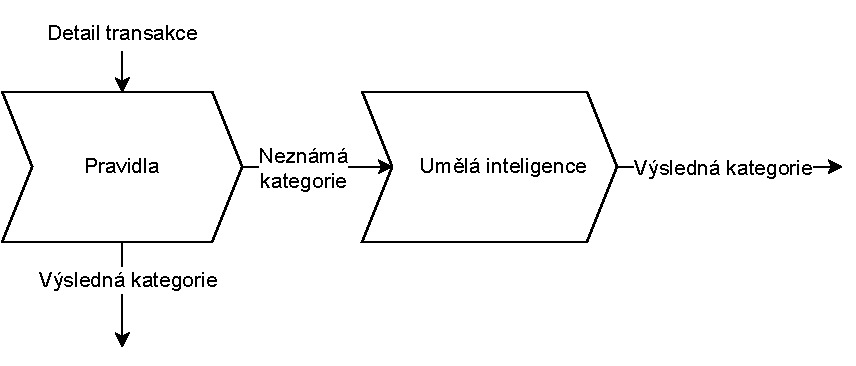
\includegraphics[width=\textwidth]{obrazky-figures/vrstvy.pdf}
\caption{Vrstvená implementace kategorizace.}
\label{fig:vrstvenaimplementace}
\end{figure}
Z~experimentu vyšlo najevo následující: Pokud použijeme testovací sadu, úspěšnost je velmi dobrá, neboť z~původních transakcí se hodně obchodních společností opakuje a~tak už byly zařazeny do pravidel. Můžeme říct, že pokud část transakce byla v~pravidlech, je úspěšnost 100 \%, pokud transakce nebyla kategorizována pravidly, je úspěšnost 70 \%. Z~toho vyplývá kombinovaná úspěšnost 85 \% ve dvouvrstvé architektuře. Uvažujeme, že v~běžném výpisu je průměrně 20-25 \% transakcí, kterou nerozezná systém pravidel a~pouze v~těchto případech bude potřeba spouštět model umělé inteligence. Tyto data jsem dostal po datové analýze mých testovacích výpisů.

\subsection{Závěr}
Po provedení těchto tří experimentů jsem došel k~závěru, že nejlepší je použit dvouvrstvou architekturu, protože předchozí experimenty ukázaly, že použití umělé inteligence ke kategorizaci transakcí nedávalo uspokojivé výsledky. V~prvním experimentu měl model obtíže s~identifikací správné kategorie, zejména pokud byl v~popisu transakce uveden pouze název nebo adresa. V~druhém experimentu, i~když si model vedl lépe po vyčištění dat, stále docházelo k~chybám při klasifikaci transakcí na základě místa. Z~experimentů vyšlo najevo, že dvouvrstvá architektura nám zajistí nejlepší výsledky a~zároveň server bude méně zatížen tím, že se nebude muset tak často provádět výpočet podobnosti v~modelu umělé inteligence.

Při každém experimentu jsem si vedl poznámky k~tomu, která kategorie byla nejčastěji špatně zařazena. Při prvním experimentu se nejčastěji netrefil u~kategorie Nákupy. V~této kategorii chyboval celkově 8krát. Ve druhém experimentu byly nejčastěji chybně zařazeny transakce kategorie Nákupy (8krát). Na rozdíl od prvního experimentu zde se zdvojnásobila chybovost u~kategorie Potraviny. Můžeme konstatovat, že pokud model nevěděl, zkoušel neznámé položky zařadit mezi kategorie, které byly zastoupeny v~datasetu častěji. Na základě těchto informací víme, že model se po úpravě datasetu choval víc předvídavě a~nesnažil se výsledky více roztrousit jak tomu bylo u~prvního experimentu. Toto chování by mohlo být považováno za významné zlepšení, neboť v~případě, že v~rámci transakce není správně rozpoznán význam určitého slova, existuje vysoká pravděpodobnost, že tato transakce spadá do kategorie nákupů či potravin, kde se vyskytuje mnoho malých prodejců.
    
\chapter{Testování}
Testování softwaru je důležitý proces při vývoji softwarových aplikací. Jeho účelem je ověřit, zda aplikace funguje tak, jak by měla, a~zda splňuje požadované specifikace a~funkční požadavky~\cite{singh2012software}. V~následujících kapitolách rozeberu jakým způsobem byla aplikace testována.
\section{Testování API}
Testování probíhalo pomocí aplikace Postman\footnote{\url{https://www.postman.com/}}. Tato aplikace umožňuje vývojářům snadno otestovat API a~získat informace o~jeho funkcích a~chování. Tato aplikace mně velmi pomohla ve zjištění, jak má API správně fungovat a~reagovat na různé požadavky. Aplikace umožňuje si předpřipravit všechny endpointy a~při každé změně v~API jedním kliknutím vyzkoušet, zda jejich odpověď odpovídá změně chování, která byla provedena. Tímto způsobem probíhalo testování API po celou dobu vývoje.
\section{Testování šablon}
Aktuálně aplikace podporuje 5 českých bank (Komerční banka, ČSOB, Moneta, AirBank, Fio). Testovací výpisy pro tyto banky se mně podařilo získat od třech na sobě nezávislých osob pro každou banku. Provedl jsem analýzu výpisu a~zaměřil se na to jak nejlépe vyextrahovat data z~těchto šablon. Následně probíhalo testování na testovacích výpisech, výpisy ve všech třech vydání se shodovali ve své specifikaci a~tak bylo testování úspěšné.
\section{Uživatelské testování}
Uživatelské testování probíhalo ve třech experimentech. Podmínkou pro účast v~testování bylo vlastnit účet u~jedné z~podporovaných bankovních společností. Podařilo se mi najít 3 testovací subjekty, každý tvořil zástupce ze své věkové kategorie (18--30 let, 30--50 let, 50+ let). Testovací subjekty jsem označil jako Testovací subjekt 1 (18--30 let), Testovací subjekt 2 (30--50 let) a~Testovací subjekt 3 (50+ let).
\subsection{Experiment č.1}
V~prvním experimentu měly testovací subjekty za úkol: Vytvořit si účet a~nahrát výpis z~minulého měsíce. U~testovacích subjektů 1 a~2 jsem nenarazil na žádnou chybu a~vše probíhalo hladce. Oba si přirozeným způsobem vytvořili účet a~nahráli své výpisy, které si dopředu stáhli z~internetového bankovnictví. U~třetího testovacího subjektu byl mírný problém s~jazykovou bariérou aplikace je celá v~angličtině a~tak starší člověk může mít problém s~jazykem, po vysvětlení základních slovíček již bylo vše v~pořádku a~experiment pokračoval. Nakonec i~třetí testovací subjekt zvládl dokončit úkol.
Na základě výsledku experimentu lze konstatovat, že experiment lze považovat za úspěšný a~základní úkol aplikace můžeme charakterizovat jako snadno zvládnutelný, jak potvrzují výsledky úspěšného absolvování úkolu všemi třemi testovacími subjekty.
\subsection{Experiment č.2}
Druhý experiment spočíval v~upravení dat na profilu a~úpravou měsíce v~daném výpisu. V~tomto experimentu splnil obě části úkolu bez nápovědy pouze testovací subjekt č.1. Následně subjekty 2 a~3 dokázaly bez problému upravit výpis. U~subjektu 2 a~3 nastaly komplikace v~hledání jak upravit profil uživatele. Po asi 2 minutách hledání jsem daným subjektům poradil, kde hledat. Tyto výsledky mě velmi překvapily a~při návrhu jsem očekával, že bude stačit informace \uv{Profile} při najetí na ikonu myší. 
Na základě výsledků druhého experimentu můžeme tvrdit, že umístnění tlačítka pro úpravu profilu není vhodné pro starší ročníky. To by se dalo změnit např. velkým navigačním tlačítkem \uv{Edit Profile}. 
%\subsection{Experiment č.3}
\subsection{Závěr}
Na základě výsledků provedených experimentů lze konstatovat, že základní principy aplikace jsou snadno zvládnutelné. Účastníci první testovací úkol zvládli bez problému, s~výjimkou jazykové bariéry u~staršího uživatele, které však byly úspěšně překonány. V~rámci druhého experimentu bylo zjištěno, že umístění tlačítka pro úpravu profilu není vhodné pro starší uživatele. Tato skutečnost pravděpodobně nezpůsobí nepoužitelnost aplikace jako celku. Celkově lze tedy říci, že aplikace v~uživatelském testování obstála a~plní svůj účel.
\chapter{Závěr}
Cílem práce bylo navrhnout a~vytvořit webovou aplikaci, která bude analyzovat transakce a~řadit je do předem určených kategorií. Hlavní myšlenkou byla snaha pomoci uživatelovi se lépe orientovat ve svých financích. Významným úspěchem v~kategorizaci transakcí je použití přístupu dvouvrstvé architektury, která dosahuje úspěšnosti 85 \%. Před samotným začátkem vývoje proběhla hloubková analýza webových frameworků a~také byly prozkoumány formáty výpisů konkrétních bankovních společnosti. Následovalo hledání vhodného způsobu jak automaticky kategorizovat transakce a~testování různých přístupů k~automatické klasifikaci. Před implementační částí práce jsem provedl návrh celé aplikace pomocí ER diagramu a~Diagramu případů užití. Dále jsem vyvinul aplikaci, ve které si uživatel vytvoří účet a~nahraje své bankovní výpisy. Tyto výpisy zařadí umělá inteligence do různých kategorií a~uživatelovi se zobrazí graf, ve kterém může pozorovat své výdaje v~různých kategorií. Uživatel může procházet již nahrané výpisy a~porovnávat grafy z~různých měsíců.

Práce mi dala nové poznatky ohledně webových frameworků na straně serveru i~klienta a~také jsem se naučil pracovat s~umělou inteligencí v~jazyce Python. Při vývoji byl kladen důraz na jednoduchost a~uživatelskou přívětivost aplikace. Také jsem se snažil zúročit všechny zkušenosti, které jsem získal v~mém studiu.

V~této práci bych chtěl dále pokračovat, protože je zde mnoho věcí ke zlepšení. Nabízí se zde možnost aplikaci obohatit o~co nejvíce bankovních společností jak z~České republiky tak ze zahraničí. Toto vylepšení je snadné na implementaci (kapitola \ref{chap:addbank}), ale časově náročné na získání informací o~struktuře výpisů a~získání testovacích výpisů. Další vylepšení by se nabízelo napojení na API bank, toto by vyžadovalo nastudovaní a~zjištění, které banky nabízí API a~zda by takový přístup byl možný v~ČR, z~důvodů smluvních podmínek bankovních společností. Dále se nabízí rozšíření o~automatické značení opakovaných plateb a~výplat. V~budoucnosti má tato práce šanci se stát oblíbenou nekomerční aplikaci pro masovou společnost. 
\\
Aplikace je dostupná online na \url{moneytracker.petrhybl.com}.
  \fi
  
  % Kompilace po částech (viz výše, nutno odkomentovat a zakomentovat input výše)
  % Compilation piecewise (see above, it is necessary to uncomment it and comment out input above)
  %\subfile{chapters/projekt-01-uvod-introduction}
  % ...
  %\subfile{chapters/projekt-05-zaver-conclusion}

  % Pouzita literatura / Bibliography
  % ----------------------------------------------
\ifslovak
  \makeatletter
  \def\@openbib@code{\addcontentsline{toc}{chapter}{Literatúra}}
  \makeatother
  \bibliographystyle{bib-styles/Pysny/skplain}
\else
  \ifczech
    \makeatletter
    \def\@openbib@code{\addcontentsline{toc}{chapter}{Literatura}}
    \makeatother
    \bibliographystyle{bib-styles/Pysny/czplain}
  \else 
    \makeatletter
    \def\@openbib@code{\addcontentsline{toc}{chapter}{Bibliography}}
    \makeatother
    \bibliographystyle{bib-styles/Pysny/enplain}
  %  \bibliographystyle{alpha}
  \fi
\fi
  \begin{flushleft}
  \bibliography{projekt-20-literatura-bibliography}
  \end{flushleft}

  % vynechani stranky v oboustrannem rezimu
  % Skip the page in the two-sided mode
  \iftwoside
    \cleardoublepage
  \fi

  % Prilohy / Appendices
  % ---------------------------------------------
  \appendix
\ifczech
  \renewcommand{\appendixpagename}{Přílohy}
  \renewcommand{\appendixtocname}{Přílohy}
  \renewcommand{\appendixname}{Příloha}
\fi
\ifslovak
  \renewcommand{\appendixpagename}{Prílohy}
  \renewcommand{\appendixtocname}{Prílohy}
  \renewcommand{\appendixname}{Príloha}
\fi
%  \appendixpage

% vynechani stranky v oboustrannem rezimu
% Skip the page in the two-sided mode
%\iftwoside
%  \cleardoublepage
%\fi
  
\ifslovak
%  \section*{Zoznam príloh}
%  \addcontentsline{toc}{section}{Zoznam príloh}
\else
  \ifczech
%    \section*{Seznam příloh}
%    \addcontentsline{toc}{section}{Seznam příloh}
  \else
%    \section*{List of Appendices}
%    \addcontentsline{toc}{section}{List of Appendices}
  \fi
\fi
  \startcontents[chapters]
  \setlength{\parskip}{0pt} 
  % seznam příloh / list of appendices
  % \printcontents[chapters]{l}{0}{\setcounter{tocdepth}{2}}
  
  \ifODSAZ
    \setlength{\parskip}{0.5\bigskipamount}
  \else
    \setlength{\parskip}{0pt}
  \fi
  
  % vynechani stranky v oboustrannem rezimu
  \iftwoside
    \cleardoublepage
  \fi
  
  % Přílohy / Appendices
  \ifenglish
    % This file should be replaced with your file with an appendices (headings below are examples only)

% For compilation piecewise (see projekt.tex), it is necessary to uncomment it and change
%\documentclass[../projekt.tex]{subfiles}
%\begin{document}

% Placing of table of contents of the memory media here should be consulted with a supervisor
%\chapter{Contents of the included storage media}

%\chapter{Manual}

%\chapter{Configuration file}

%\chapter{Scheme of RelaxNG configuration file}

%\chapter{Poster}

\chapter{How to use this template}
\label{jak}

This chapter describes individual parts of the template, followed by a brief instructions on how to use it. If you have any questions, comments etc, feel free to email them to \texttt{sablona@fit.vutbr.cz}.

\section*{Template parts description}

Once you extract the template, you will find the following files and directories:
\begin{DESCRIPTION}
  \item [bib-styles] Literature styles (see below). 
  \item [obrazky-figures] Directory for your images. Currently contains \texttt{placeholder.pdf} (a.k.a TODO image -- see below) and image keep-calm.png to demonstrate inserting raster images (you don't submit these images with your thesis). It is advised to use shorter directory name, so that it is only in your chosen language.
  \item [template-fig] Template images (BUT logo).
  \item [fitthesis.cls] Template (design definition).
  \item [Makefile] Makefile used to compile the project, count standard pages etc. (see below).
  \item [projekt-01-kapitoly-chapters-en.tex] File for Your text (replace it's contents).
  \item [projekt-20-literatura-bibliography.bib] Reference list (see below).
  \item [projekt-30-prilohy-appendices-en.tex] File for your appendices (replace it's contents).
  \item [projekt.tex] Main project file -- definitions of formal parts.
\end{DESCRIPTION}

The style of literature in the template is from Ing. Radek Pyšný \cite{Pysny}, whose work was improved by prof. Adam Herout, dr. Jaroslav Dytrych and Mr. Karel Hanák to comply with the norm and support all frequently used types of citations. Its documentation can be found in the appendix

Aside from compilation to PDF, the Makefile also offers additional functions:
\begin{itemize}
  \item rename files (see below),
  \item count standard pages,
  \item run a wave that adds unbreakable spaces,
  \item compress (zip) the result, ready to be sent to your supervisor and checked (make sure that all the files you've added are included, if not, add them manually).
\end{itemize}

Keep in mind that the wave is not perfect. You always need to check whether or not there is something inappropriate at the end of a line manually -- see Online language handbook\footnote{Internetová jazyková příručka \url{http://prirucka.ujc.cas.cz/?id=880}}.

Similar rules apply also in English - see eg. article Run Ragged\footnote{Run Ragged\url{https://24ways.org/2013/run-ragged/}}, according to which there should be no prepositions, dash or short words (2--3 letters) at the end of the lines, the two lines following each other should not end with a comma and line break should not be also in the phrases from 2-3 words.

\paragraph {Pay attention to page numbering!} If the table of contents is 2 pages long and the second page contains only \uv{Enclosures} and \uv{List of enclosures} (but there is no enclosure), the page numbering is changed by 1 (table of contents and contents \uv{mismatch}). The same thing happens if the second or third page contains only \uv{References} and there's a chance that this can occur in other situations too. There are multiple solutions to this (from editing the table of contents, setting the page counter all the way to more sophisticated methods). \textbf{Check the page numbering before you submit your thesis!}

\section*{Recommendations for working with the template}

\begin{enumerate}
  \item \textbf{Make sure you have the latest version of template.} If you have a template from last year, there should be a newer version (updated information, fixed errors etc.) available at the faculty or study advisor web pages.  
  \item \textbf{Choose a language}, that you want to use for your technical report (czech, slovak or english) and consult your supervisor about your choice (unless it was agreed upon in advance). If your language of choice is not czech, set the respective template parameter in file projekt.tex (e.g.: \verb|document|\verb|class[english]{fitthesis}| and translate the declaration and acknowledgement to english or slovak).
  \item \textbf{Rename the files.} When you extract the files, there should be a file named projekt.tex. If you compile it, it will create a PDF with technical report named projekt.pdf. If multiple students send their supervisor projekt.pdf to have it checked, they have to rename them. For that reason, it is advised to rename the file so that it contains your login and (if needed, abbreviated) work topic. Avoid using spaces, diacritic and special symbols. An appropriate name for your file can look like this: \uv{xlogin00-Cleaning-and-extraction-of-text.tex}. You can use the included Makefile to rename it: 
\begin{verbatim}
make rename NAME=xlogin00-Cleaning-and-extraction-of-text
\end{verbatim}
  \item Fill in the required information in file, that was originally named projekt.tex, that means type, year (of submission), thesis title, author's name, department (according to specification), supervisor's titles and name, abstract, keywords and other formal requirements.
  \item Replace the contents of thesis chapters, references and enclosures files with the contents of your technical report. Individual enclosures or thesis chapters can be saved to separate files -- if you choose this approach, it is advised to comply with the file naming convention, and the number will be followed by the chapter title.
  \item If you don't need enclosures, comment the respective part in projekt.tex and erase everything from the corresponding file or delete it. Don't try to come up with an aimless enclosures just to have something in that file. An appropriate enclosure can be the contents of included memory medium.
  \item Delete the chapter and attachment files for a language you haven't used (with or without \texttt{-en}).
  \item Assignment that you download in PDF from BUT IS (link \uv{Thesis assignment}) save to file \texttt{zadani.pdf} and enable its insertion into work by appropriate template parameter (\verb|document|\verb|class[zadani]{fitthesis}|) in \texttt{projekt.tex}.
  \item If you don't want to print references in color (i cannot recommend this without consulting your supervisor), you'll need to create a second PDF for printing and set the template printing parameter:\\ (\verb|document|\verb|class[english,zadani,print]{fitthesis}|). Colored logo must not be printed in black and white.
  \item The binder templace where the thesis will be typeset can be generated in faculty IS at specification. Can be enabled for dissertation using the \tt cover \rm parameter in template.
  \item Don't forget that source files and (both versions) PDF has to be on a CD or other medium included in the technical report.
\end{enumerate}

\subsection*{Instructions for double-sided printing}
\begin{itemize}
\item \textbf{It is advised to consult your supervisor about double-sided printing.}
\item If you used double-sided printing for your thesis and it's thickness is smaller than the thickness of the binder, it doesn't look too good.
\item Enabled using the following template parameter:\\ \verb|\document|\verb|class[twoside]{fitthesis}|
\item After printing a double-sided sheet, make sure that the canon of page construction is in the same position on both pages. Inferior printers with duplex printing unit usually cause a shift by 1--3 mm. This can be solved with some printers. Print the odd pages first, put them back into the same tray and print the even pages.
\item Leave a blank page after title page, table of contents, references, list of tables, list of appendices and other lists to make sure that the following part starts on an odd page (\texttt{\textbackslash cleardoublepage}).
\item Check the final result thoroughly.
\end{itemize}

\subsection*{Paragraph style}

Paragraphs have justified alignment and there are multiple methods for formatting them. In Czech paper literature, a paragraph indentation method is common, where each paragraph of the text have the first line of a paragraph indented by about one to two quads, that is, about two widths of the capital letter M of the base text (always about the same preselected value). In this case, the last line of the previous paragraph and the first line of the following paragraph are not separated by a vertical space. The interleaving between these lines is the same as the interleaving inside the paragraph \cite{fitWeb}.

Another method is indenting paragraphs, which is common for electronic typesetting and for English texts. In this method, the first line of a paragraph is not indented and a vertical space of approximately half of a line is inserted between the paragraphs. Both methods can be used in the thesis, however, the latter method is often more suitable. Methods should not be combined.

One of the above methods is set as the default in the template, the other can be selected by the template parameter \uv{\tt odsaz\rm }.


\subsection*{Useful tools} 
\label{nastroje}

The following list is not a list of all useful tools. If you have experience with a certain tool, feel free to use it. However, if you don't know which tool to choose, consider the ones listed below:

\begin{description}
	\item[\href{http://miktex.org/download}{MikTeX}] \LaTeX{} for Windows -- a distribution with simple installation and great automated package downloading. MikTeX even has it's own editor, but I highly recommend TeXstudio.
	\item[\href{http://texstudio.sourceforge.net/}{TeXstudio}] Portable opensource GUI for \LaTeX{}. Ctrl+click switches between source text and PDF. Integrated spell checker\footnote{Spell checker for czech version can be installed from \url{https://extensions.openoffice.org/de/project/czech-dictionary-pack-ceske-slovniky-cs-cz}}, syntax highlighter etc. To use this tool, you need to first install MikTeX or another \LaTeX{} distribution.
    \item[\href{http://www.winedt.com/}{WinEdt}] A good combination for Windows is WinEdt + MiKTeX. WinEdt is a GUI for Windows, and if you want to use it, you need to first install \href{http://miktex.org/download}{MikTeX} or \href{http://www.tug.org/texlive/}{TeX Live}.
    \item[\href{http://kile.sourceforge.net/}{Kile}] Editor for KDE (Linux) desktop environment. Real-time preview. To use this tool, you need to have \href{http://www.tug.org/texlive/}{TeX Live} and Okular installed.
	\item[\href{http://jabref.sourceforge.net/download.php}{JabRef}] Neat and simple Java program for bibliography (references) file management. No need to learn anything -- provides a simple window and a form for entry editing.
	\item[\href{https://inkscape.org/en/download/}{InkScape}] Portable opensource vector graphic (SVG and PDF) editor. Excellent tool to use to create images for technical text. Difficult to master, but the results are worth it.
	\item[\href{https://git-scm.com/}{GIT}] Great tool for teamwork when it comes to projects, but can be incredibly useful even to a single author. Simple version control system, backup options and transfer between multiple computers.
	\item[\href{http://www.overleaf.com/}{Overleaf}] Online \LaTeX{} tool. A real-time compilation of source text that allows for simple collaboration (supervisor can continuously keep an eye on the progress made), move to a place in source file just by clicking in the PDF preview, spell checker etc. There are some limitations to what you can do if you want to use it for free (some people are comfortable with it for dissertation, others can run into it while they write a~bachelor's thesis) and it is rather slow for long texts. FIT BUT has for students and employees of a license, which can be activated on \url{https://www.overleaf.com/edu/but}.
\end{description}

Note: Overleaf does not use template Makefile -- to get compilation to work, you need to go to the menu and select \tt projekt.tex \rm as s Main document.

\chapter{Writing english texts}
\label{anglicky}
This chapter is taken from web pages of Jan Černocký \cite{CernockyEnglish}.

A lot of people write their technical reports in english (which is good!), but they make a~lot of unnecesary mistakes (which is bad!). I'm not an english export myself, but I've been using this language for a while now to write, read and even communicate -- this chapter contains a handful of important things. If you want to be certain that your thesis or article is 100\,\% correct, your best bet is to hire a native speaker (preferably someone who is technically capable and understands what you write about \ldots).


\section*{In general}

\begin{itemize}
  \item{Before you jump into it head first, I suggest you read a handful of technical articles written in english and try to remember or preferably understand how you should approach writing one yourself.}
  \item{Always use a spell checking tools -- built in tools in Word, or in OpenOffice. If you work on Linux, I suggest you use ISPELL. Some spell checking (I think it's the one in PSPad) are not very good and ignore a lot of mistakes.}
  \item{Use grammer checking tools. I'm not entirely sure if there is one available for Linux, but the one in Word is fairly decent and if it underlines anything with green color, it's probably wrong. You can even copy and paste Latex source code here, fix any and all grammar errors and save it as a clean text again. If you use vim, there's a~built in grammar checking tool too, and it's capable of detecting typos and errors in basic grammar. Write this in the first line of your thesis tex file:
  \begin{verbatim}
    % vim:spelllang=en_us:spell
  \end{verbatim}
  (alternatively \texttt{en\_gb} for OED english) \textit{Editor's note:} There is a very good online tool Grammarly\footnote{\url{https://www.grammarly.com/}}, with free basic version.
  }
  \item{Online dictionaries are good, but don't rely on them in every situation. Usually you get multiple choices and not all of them are correct for the given context.}
  \item{\begin{samepage}You can probably figure out what the correct option is by looking each option up and seeing the context in which they're used, example given: ``advantage/privilege/facility of approach''. Online dictionaries give you a handful of results. Look them up one by one using google search:
  \begin{verbatim}
    "advantage of this approach" 1100000 hits
    "privilege of this approach" 6 hits
    "facility of this approach"  16 hits
  \end{verbatim}
  I'm not saying it's 100\,\% correct, but at least you have something to go on. This can be used to find the correct connectives (e.g. ``among two cases'' or ``between two cases''?)\end{samepage}}
\end{itemize}
       
\section*{SVOMPT and concord}

The structure of an english sentence is SVOPMT: SUBJECT VERB OBJECT MANNER PLACE TIME and there's no other way around it. It is not a flexible structure. There are possibly exceptions in things like a theater play, where something needs to be emphasized. Subject must be present in every single single sentence, people tend to forget as some languages have a sentence structure where the subject can be implicit and not mentioned. SVOMPT applies to dependent clauses too!
\begin{verbatim}
  BAD: We have shown that is faster than the other function. 
  GOOD: We have shown that it is faster than the other function. 
\end{verbatim}

\noindent Concord or grammatical agreement between two words in a sentence -- it sounds silly, but people make countless mistakes here.

\begin{verbatim}
  he has 
  the users have 
  people were 
\end{verbatim}

\section*{Articles}

Articles in english are a nightmare and almost all of us fail to use them correctly. The basic rule is, that if there's a particular noun, it's preceeded by ``the''. Definite articles must be in following phrases:
\begin{verbatim}
  the first, the second, ...
  the last
  the most (superlatives and adverbs) ...
  the whole 
  the following 
  the figure, the table. 
  the left, the right - on the left pannel, from the left to the right ... 
\end{verbatim}

\noindent On the contrary, there can't be an article when you're referring to a specific figure, chapter, etc.
\begin{verbatim}
  in Figure 3.2
  in Chapter 7
  in Table 6.4
\end{verbatim}

\begin{samepage}
\noindent The use of ``a'' and ``an'' is based on the pronounciation, rather than how the word is written:
\begin{verbatim}
  an HMM
  an XML
  a universal model
  a user
\end{verbatim}
\end{samepage}

\section*{Verbs}

Passive voice can be tricky -- regular verbs are usually not a problem, irregular verbs however are a common source of errors, typically
\begin{verbatim}
  packet was sent (rather than send)
  approach was chosen (rather than choosed)
\end{verbatim}
\noindent \ldots most of the time, the spell checker will correct it, but it's not guaranteed.

Tenses are a mess at times. If something just is in general, use present tense. If you did something, use past tense. If you got results that already exist and you just discuss them, use present tense. Try to avoid complicated tenses such as present perfect or worse past perfect if you're not 100\,\% sure.
\begin{verbatim}
  JFA is a technique that works for everyone in speaker recognition. 
  We implemented it according to Kenny's recipe in \cite{Kenny}. 
  12000 segments from NIST SRE 2006 were processed. When compared 
  with a GMM baseline, the results are completely bad. 
\end{verbatim}

\section*{Sentence length and structure}

\begin{itemize}
  \item{Try to write shorter sentences. If you sentence is 5 lines long, it's probably a pain to read, if it can even be done.}
  \item{Comma is a powerful tool and you should use it for your sentence structure. Use a~comma to seperate the initial dependent clause from the main independent clause. Sometimes it is appropriate to put a comma just before ``and'' (unlike other languages)!}
\end{itemize}
\begin{verbatim}
  In this chapter, we will investigate into ... 
  The first technique did not work, the second did not work as well, 
  and the third one also did not work. 
\end{verbatim}

\section*{The specifics of a technical text}

When writing a technical text, don't use common phrases such as
\begin{verbatim}
  he's
  gonna
  Petr's working on ...
\end{verbatim}
\noindent and others. The only tolerated thing is ``doesn't'', but you can never go wrong with ``does not''.

\begin{samepage}
\noindent Technical texts utilize passive voice a lot more than active voice: 
\begin{verbatim}
  BAD: In this chapter, I describe used programming languages. 
  GOOD: In this chapter, used programming languages are described.
\end{verbatim}
\end{samepage}

If you want to use active voice, it's more common to use ``we'', even though you work alone. ``I'', ``my'', etc. are only used when you need to emphasize that you are the person of utmost importance, for example in the conclusion or when discussing ``original claims'' in disertation.


\paragraph{Common erros in words}

\begin{itemize}
  \item{Pay attention to his/hers, it's not ``it's'' but ``its''}
  \item{Image is not picture, it's figure.}
  \item{The connective is ``than'', not ``then'' -- bigger than this, smaller than this \ldots very common error! ``Then'' is used in the context of time.}
\end{itemize}


\chapter{Checklist}
\label{checklist}
This checklist was taken from a template for academic work, that is available on Adam Herout's blog \cite{Herout}, based on the ideas of Igor Szöke\footnote{\url{http://blog.igor.szoke.cz/2017/04/predstartovni-priprava-letu-neni.html}}, with their permission.

A big part of the safety of air transport are checklists. They have checklists for basically anything and everything, even the most cut-and-dry procedures. If a pilot can get over the tedious process of marking off every single checkbox of a procedure, you can as well. Make a checklist of your own before you submit your thesis. \bf Yes, really: \rm print it, grab a pencil and check every single item on the list. It will make your life easier –- avoid unnecessary errors that can be fixed within a couple minutes –- as well as others', at very least your supervisor and reviewer of your thesis.

\subsection*{Structure}
\begin{checklist}
	\item You can tell that the assignment was completed just by looking at the chapter titles as well as their structures.
    \item There is no chapter with less than four pages (except for introduction and conclusion). And if so, I discussed this with my supervisor and they gave me a green light.
\end{checklist}

\subsection*{Figures and charts}
\begin{checklist}
	\item Every single image and table was checked and their position is close to the text that references them. In other words, they’re easy to find.
    \item Every single image and table has a good enough caption, to ensure that the figure makes sense on it’s own, without the necessity to read the text. (There’s no harm in a long caption.)
    \item If an image is taken from somewhere, it is mentioned in the caption: “Taken from [X].”
    \item Texts in all images have a font size similar to the surrounding text (neither signifficantly larger, nor signifficantly smaller).
    \item Charts and schemes are vector graphics (eg. in PDF).
    \item Screenshots don‘t use lossy compression (they‘re in PNG).
    \item All images are referenced in the text.
    \item Axes in charts have their captions (name of the axis, units of measurement, values) and a grind if need be.
\end{checklist}

\subsection*{Equations}
\begin{checklist}
	\item Identifiers and their indexes in equations are single letters (except for rather uncommon cases like $t_{max}$).
    \item Equations are numbered.
    \item All the variables and functions that haven‘t been explained yet are explained below (or rarely above) the equation.
\end{checklist}

\subsection*{Citations}
\begin{checklist}
	\item \bf All used sources are cited. \rm
	\item URL adresses referencing services, projects, sources, github, etc. are referenced using \verb|\footnote{\url{…}}|.
    \item URL adresses in citations are only present, if necessary – article is cited like an article (author, title, where and when was it published), not using URL.
    \item Citations have author, title, publisher (conference title), year of publishing. If a~citation does not have either of these, there is a good explanation for this special case and my supervisor agreed.
    \item If there is anything taken over from some other work in the program source code, it is properly cited therein in conformance with the license.
	\item If an essential part of the source code of the program is taken over, this is mentioned in the text of the thesis and the source is cited.
\end{checklist}

\subsection*{Typography}
\begin{checklist}
	\item No line extends past the right margin.
    \item There is no single-letter preposition at the end of a line (fixed using unbreakable space \verb|~|).
    \item Number of image, table, equation, citation is never a first item of a new line (fixed using unbreakable space \verb|~|).
    \item There is no space before a numeric reference to a footnote (like this\footnote{footnote example}, not like this \footnote{another footnote example}).
\end{checklist}

\subsection*{Language}
\begin{checklist}
	\item I used spellchecker and there were no typos in the text.
    \item I had someone else read my thesis (at least one person), that knows czech / slovak / english well.
    \item Someone who knows english well checked the abstract  in a czech or slovak written abstract thesis.
    \item No part of the text is written in second person (you).
    \item If first person is used (i, we), a subjective matter is being described (i decided, i~designed, i focused on, i found out, etc.).
    \item There are no colloquialisms in the text.
    \item There are no {\it default} words in the text.
\end{checklist}

\subsection*{Result is on a data medium, i.e. software}
\begin{checklist}
	\item I have a non-rewritable data medium ready.
    \begin{itemize}
    	\item CD-R,
        \item DVD-R,
        \item DVD+R in ISO9660 format (with RockRidge and/or Jolliet extension) or UDF,
        \item SD (Secure Digital) card in FAT32 or exFAT format, the card is set to write-protected mode
    \end{itemize}
    \item If the result is online (service, application, …), URL is visible in introduction and conclusion.
    \item The medium contains the following mandatory items:
    \begin{itemize}
    	\item source codes (e.g. Matlab, C/C++, Python, \ldots)
        \item libraries necessary for compilation,
        \item compiled solution,
        \item PDF containing a technical report,
        \item text source code (\LaTeX{}),
    \end{itemize}
    and the following optional items after consulting your supervisor:
    \begin{itemize}
    	\item relevant (e.g. testing) data,
        \item demo video,
        \item poster in PDF
        \item \ldots
    \end{itemize}
    \item Source codes are refactorized, commented and labelled with an authorship header so that others can tell what they actually are.
    \item Any and all snippets of code taken from another sources are properly cited -- differentiated using a opening and in case of multiple lines of code a closing comment. Comments contain everything that the license on web (always try to find out what the license is -- for example, Stack Overflow\footnote{\url{https://stackoverflow.blog/2009/06/25/attribution-required/}} has a very strict citation policy).
\end{checklist}

\subsection*{Submission}
\begin{checklist}
	\item Do I want to delay (by at most 3 years) the publication ? If so, I will submit an application (in IS) at least a month prior to the submission of the academic work, and I'll include attitude of the company that the intellectual property belongs to and needs to be protected.
    \item I have at least minimum number of standard pages (can be calculated using Makefile and by adding number of pages that images translate to). If I'm just under the minimum, I consulted my supervisor about it.
   	\item If I want a two-sided print, I consulted my supervisor about it and I've used correct template settings for two-sided printing. Chapters begin on odd pages.
    \item Technical report is bound in a bookbindery (at least one print, both prints if I'm delaying the publishing).
    \item Title page is followed by the specification (in other words, downloaded from IS and inserted into the template)
    \item Abstract and keywords are uploaded in IS.
      \begin{itemize}
        \item There are no \verb|~| characters for non-breaking spaces in the abstract and keywords in IS.
      \end{itemize}     
    \item PDF of thesis (with clickable links) is in IS.
    \item Both prints are signed.
    \item One (both if I'm delaying the publishing) of the prints contains a data medium with my login written on it using a CD marker (CD marker can be borrowed in library, at Student affairs or when I'm submitting the work).
\end{checklist}

\chapter{\LaTeX{} for beginners}
\label{latex}

This chapter contains commonly used \LaTeX{} packages and commands, that you might need when you're developing a thesis.

\subsection*{Useful packages}

Students usually encounter the same issues. Some of them can be solved using the following \LaTeX{} packages:

\begin{itemize}
  \item \verb|amsmath| -- additional equation typesetting options,
  \item \verb|float, afterpage, placeins| -- image placement,
  \item \verb|fancyvrb, alltt| -- change the properties of Verbatim environment, 
  \item \verb|makecell| -- additional table options,
  \item \verb|pdflscape, rotating| -- rotate a page by 90 degress (for image or table),
  \item \verb|hyphenat| -- change how words break,
  \item \verb|picture, epic, eepic| -- direct image drawing.
\end{itemize}

Some packages are used in this very template (in the lower section of fitthesis.cls file). It is also advised to read the documentation for individual packages.

A table column aligned to left with a fixed width is defined as "L" in the template (used as "p").

To reference a place within text, use command \verb|\ref{label}|. Depending on the placement of this label, it will be a number of chapter, subchapter, image, table or a similar numbered element. If you want to reference a specific page, use command \verb|\pageref{label}|. To cite a literature reference, use command \verb|\cite{identifier}|. To reference an equation, you can use command \verb|\eqref{label}|.

Symbol -- (dash) is used generated using two minus signs (like this: \verb|--|) in \LaTeX.

\subsection*{Commonly used \LaTeX{} commands}
\label{sec:Fragments}

I highly recommend you check the source text of this chapter and see how the following examples are created. The source text even contains helpful comments.

% A left-aligned, fixed-width column is defined in the template as "L" (used as p).

Example table:
\begin{table}[H]
	\vskip6pt
	\caption{Assessment table}
    \vskip6pt
	\centering
	\begin{tabular}{llr}
		\toprule
		\multicolumn{2}{c}{Name} \\
		\cmidrule(r){1-2}
		Name & Surname & Assessment \\
		\midrule
		Jan & Novák & $7.5$ \\
		Petr & Novák & $2$ \\
		\bottomrule
	\end{tabular}
	\label{tab:ExampleTable}
\end{table}

% Ohraničení lze upravit dle potřeby:
% http://latex-community.org/forum/viewtopic.php?f=45&t=24323
% http://tex.stackexchange.com/questions/58163/problem-with-multirow-and-table-cell-borders
% http://tex.stackexchange.com/questions/79369/formatting-table-border-and-text-alignment-in-latex-table

\noindent Example equation:
\begin{equation}
\cos^3 \theta =\frac{1}{4}\cos\theta+\frac{3}{4}\cos 3\theta
\label{rovnice2}
\end{equation}
and two horizontally aligned equations: % znak & řídí zarovnání
\begin{align} \label{eq:soustava}
	3x &= 6y + 12 \\
	x &= 2y + 4 
\end{align}

If you need to reference an equation from the text, you can use command \verb|\eqref|. For example, to reference the equations above \eqref{rovnice2}. If you want to align the equation number vertically, you can use command \texttt{split}:

\begin{equation} \label{eq:soustavaSrovnana}
\begin{split}
	3x &= 6y + 12 \\
	x &= 2y + 4
\end{split}
\end{equation}

Mathematical symbols ($\alpha$) and expressions can be placed even in text $\cos\pi=-1$ and can also be in a footnote%
\footnote{Formula in a footnote: $\cos\pi=-1$}.

Image~\ref{sirokyObrazek} displays a wide image comprised of multiple smaller images. Standard raster image is inserted in the same way as image \ref{keepCalm}.

% Využití \begin{figure*} způsobí, že obrázek zabere celou šířku stránky. Takový obrázek dříve mohl být pouze na začátku stránky, případně na konci s využitím balíčku dblfloatfix (případné [h] se ignorovalo a [H] obrázek odstraní). Nové verze LaTeXu už umí i [h].
\begin{figure*}[h]\centering
  \centering
  \includegraphics[width=\linewidth,height=1.7in]{obrazky-figures/placeholder.pdf}\\[1pt]
  \includegraphics[width=0.24\linewidth]{obrazky-figures/placeholder.pdf}\hfill
  \includegraphics[width=0.24\linewidth]{obrazky-figures/placeholder.pdf}\hfill
  \includegraphics[width=0.24\linewidth]{obrazky-figures/placeholder.pdf}\hfill
  \includegraphics[width=0.24\linewidth]{obrazky-figures/placeholder.pdf}
  \caption{\textbf{Wide image.} Image can be comprised of multiple smaller images. If you want to address the partial images from text, use packagae \texttt{subcaption}.}
  \label{sirokyObrazek}
\end{figure*}

% Uncomment this to switch to landscape oriented A3 paper
% \eject \pdfpagewidth=420mm

\begin{figure}[hbt]
	\centering
	\includegraphics[width=0.3\textwidth]{obrazky-figures/keep-calm.png}
	\caption{Good text is a bad text, that has been changed countless times. You have to start somewhere.}
	\label{keepCalm}
\end{figure}

Sometimes it is necessary to attach a diagram that does not fit on an A4 page. Then it is possible to insert one A3 page and fold it into the thesis (so-called Engineering fold, similar to Z-fold, where two folds are created -- face down and face up). Switching is performed as follows: \texttt{\textbackslash{}eject \textbackslash{}pdfpagewidth=420mm} (210mm to switch it back).

Other frequently used commands can be found above in the text, because a single practical example of correct use is better than ten pages of examples.

% Uncomment this to switch back to A4
% \eject \pdfpagewidth=210mm


% newline command
\newcommand{\odradkovani}{\\[0.3em]}

\chapter{Examples of bibliographic citations}
\label{priloha-priklady-citaci}
The czplain style is based on the style created by mr. Pyšný \cite{Pysny}. This appendix contains a set of supported type of citations with specific examples of bibliograhpic citations.

The next pages of the appendix contain examples of bibliographic citations of the following pubplications and their parts:
\begin{itemize}
   \item Article in a periodical literature (magazine) (str. \pageref{pr-casopis-clanek}),
   \item monographic publication (str. \pageref{pr-monografie}),
   \item conference proceedings (str. \pageref{pr-sbornik}),
   \item conference proceedings entry or book chapter (str. \pageref{pr-kapitola}),
   \item manual, documentation, technical report and unpublished materials (str. \pageref{pr-manual}),
   \item academic work (str. \pageref{pr-thesis}),
   \item web page (str. \pageref{pr-webpage}),
   \item and web site (str. \pageref{pr-website}).
\end{itemize}

\noindent Items are color-coded depending on whether or not they are required or optional:
\begin{itemize}
    \item required element according to the standard
    \item \textcolor{blue}{optional element according to the standard}
    \item \textcolor{magenta}{required element for online information sources according to the standard}
    \item \textcolor{red}{element that is not specified in the standard, but is available and optional within the template's bibliographic style}
\end{itemize}
Required items are only stated if they exist.

\newpage
The bibliography file contains records in the following form:
\begin{verbatim}
@Article{Doe:2020,
   author               = "Doe, John",
   title                = "How to cite",
   subtitle             = "Article citation",
   journal              = "Writing theses and dissertations",
   journalsubtitle      = "Formal aspects",
   howpublished         = "online",
   address              = "Brno",
   publisher            = "Brno University of Technology, 
                          Faculty of information technology",
   contributory         = "Translated by Jan NOVÁK",
   edition              = "1",
   version              = "version 1.0",
   month                = 2,
   year                 = "2020",
   revised              = "revised 12. 2. 2020",
   volume               = "4",
   number               = "24",
   pages                = "8--21",
   cited                = "2020-02-12",
   doi                  = "10.1000/BC1.0",
   issn                 = "1234-5678",
   note                 = "This a made up citation",
   url                  = "https://merlin.fit.vutbr.cz"
}
\end{verbatim}


%-------------------------------------------------------------------------------
\newpage
\section*{Article in a periodical literature -- @Article}
\label{pr-casopis-clanek}
\noindent \textbf{Record items}

\medskip

\begin{tabularx}{0.95\linewidth}{>{\raggedright\arraybackslash}X X >{\raggedright\arraybackslash}X}
    Element & BibTeX item & Example\\\hline
    Author & author & Doe, John\\
    Article title & title & How to cite\\
    \textcolor{blue}{Article subtitle} & \textcolor{blue}{subtitle} & \textcolor{blue}{Article citation}\\
    Periodical literature title & journal & Writing theses and dissertations\\
    \textcolor{blue}{Periodical literature subtitle} & \textcolor{blue}{journalsubtitle} & \textcolor{blue}{Formal aspects}\\
    \textcolor{magenta}{Type of medium} & \textcolor{magenta}{howpublished} & \textcolor{magenta}{online}\\
    Edition & edition & 1\\
    Version & version & version 1.0\\
    \textcolor{blue}{Secondary author(s)} & \textcolor{blue}{contributory} & \textcolor{blue}{Translated by Jan NOVÁK}\\
    Place of publication & address & Brno\\
    Publisher & publisher & Brno University of Technology, Faculty of information technology\\
    Month & month & 2\\
    Year & year & 2020\\
    Volume & volume & 4\\
    Number & number & 24\\
    Pages & pages & 8-21\\
    Revision & revised & revised 12. 2. 2020\\
    \textcolor{magenta}{Date of citation} & \textcolor{magenta}{cited} & \textcolor{magenta}{2020-02-12}\\
    Series title & series & Guidelines for writing theses and dissertations\\
    Number in series & editionnumber & 42\\
    \textcolor{magenta}{Digital object identifier} & \textcolor{magenta}{doi} & \textcolor{magenta}{10.1000/BC1.0}\\
    Standard number & issn & 1234-5678\\
    \textcolor{red}{Notes} & \textcolor{red}{note} & \textcolor{red}{This is a made up citation}\\
    \textcolor{magenta}{Availability} & \textcolor{magenta}{url} & \textcolor{magenta}{https://merlin.fit.vutbr.cz}
\end{tabularx}

\bigskip

\noindent \textbf{Bibliographic citation}

\medskip

\noindent \textsc{Doe}, J. How to cite: Article citation. \textit{Writing theses and dissertations: Formal aspects} [online]. 1st ed., version 1.0. Translated by Jan NOVÁK. Brno: Brno University of Technology, Faculty of information technology. February 2020, vol. 4, num. 24, p. 8–21, revised 12. 2. 2020, [cit. 2020-02-12]. Guidelines for writing theses and dissertations, no. 42. DOI: 10.1000/BC1.0. ISSN 1234-5678. This is a made up citation. Available at: \url{https://merlin.fit.vutbr.cz}

%-------------------------------------------------------------------------------
\newpage
\section*{Monographic publication -- @Book, @Booklet (brochure)}
\label{pr-monografie}
\noindent \textbf{Record items}

\medskip

\begin{tabularx}{0.95\linewidth}{>{\raggedright\arraybackslash}X X >{\raggedright\arraybackslash}X}
    Element & BibTeX item & Example\\\hline
    Author & author & John von Doe\\
    Title & title & How to cite\\
    \textcolor{blue}{Subtitle} & \textcolor{blue}{subtitle} & \textcolor{blue}{Monographic publication citation}\\
    \textcolor{magenta}{Type of medium} & \textcolor{magenta}{howpublished} & \textcolor{magenta}{online}\\
    Edition & edition & 1\\
    \textcolor{blue}{Secondary author(s)} & \textcolor{blue}{contributory} & \textcolor{blue}{Translated by Jan NOVÁK}\\
    Place of publication & address & Brno\\
    Publisher & publisher & Brno University of Technology, Faculty of information technology\\
    Month & month & 2\\
    Year & year & 2020\\
    Revision & revision & revised 12. 2. 2020\\
    \textcolor{magenta}{Date of citation} & \textcolor{magenta}{cited} & \textcolor{magenta}{2020-02-12}\\
    \textcolor{red}{Pages} & \textcolor{red}{pages} & \textcolor{red}{220}\\
    Series title & series & Guidelines for writing theses and dissertations\\
    Number in series & editionnumber & 2\\
    Standard number & isbn & 01-234-5678-9\\
    \textcolor{red}{Notes} & \textcolor{red}{note} & \textcolor{red}{This is a made up citation}\\
    \textcolor{magenta}{Availability} & \textcolor{magenta}{url} & \textcolor{magenta}{https://merlin.fit.vutbr.cz}\\
\end{tabularx}

\bigskip

\noindent \textbf{Bibliographic citation}

\medskip

\noindent \textsc{von Doe}, J. \textit{How to cite: Monographic publication citation} [online]. 1st ed. Translated by Jan NOVÁK.
Brno: Brno University of Technology, Faculty of information technology, February 2020, revised 12. 2. 2020 [cit. 2020-02-12]. 220 p. Guidelines for writing theses an dissertations, no. 2. ISBN 01-234-5678-9. This is a made up citation. Available at: \url{https://merlin.fit.vutbr.cz}
%-------------------------------------------------------------------------------
\newpage
\section*{Conference proceedings -- @Proceedings}
\label{pr-sbornik}
\noindent \textbf{Record items}

\medskip

\begin{tabularx}{0.95\linewidth}{X X >{\raggedright\arraybackslash}X}
    Element & BibTeX item & Example\\\hline
    \textcolor{red}{Author*} & \textcolor{red}{author} & \textcolor{red}{Čechmánek, Jan}\\
    \textcolor{red}{Editor*} & \textcolor{red}{editor} & \textcolor{red}{Čechmánek, Jan}\\
    Title & title & How to cite\\
    \textcolor{blue}{Subtitle} & \textcolor{blue}{subtitle} & \textcolor{blue}{Conference proceedings citation}\\
    \textcolor{magenta}{Type of medium} & \textcolor{magenta}{howpublished} & \textcolor{magenta}{online}\\
    Edition & edition & 1\\
    \textcolor{blue}{Secondary author(s)} & \textcolor{blue}{contributory} & \textcolor{blue}{Translated by Jan NOVÁK}\\
    Place of publication & address & Brno\\
    Publisher & publisher & Brno University of Technology, Faculty of information technology\\
    Month & month & 2\\
    Year & year & 2020\\
    Volume & volume & 4\\
    Number & number & 24\\
    Pages & pages & 8-21\\
    \textcolor{magenta}{Revision} & \textcolor{magenta}{revised} & \textcolor{magenta}{revised 12. 2. 2020}\\
    \textcolor{magenta}{Date of citation} & \textcolor{magenta}{cited} & \textcolor{magenta}{2020-02-12}\\
    Series title & series & Guidelines for writing theses and dissertations\\
    Number in series & editionnumber & 2\\
    \textcolor{magenta}{Digital object identifier} & \textcolor{magenta}{doi} & \textcolor{magenta}{10.1000/BC1.0}\\
    Standard number & isbn or issn & 01-234-5678-9\\
    \textcolor{red}{Notes} & \textcolor{red}{note} & \textcolor{red}{This is a made up citation}\\
    \textcolor{magenta}{Availability} & \textcolor{magenta}{url} & \textcolor{magenta}{https://merlin.fit.vutbr.cz}
\end{tabularx}

*Either author or editor is stated.

\bigskip

\noindent \textbf{Bibliographic citation}

\medskip

\noindent \textsc{Čechmánek}, J. \textit{How to cite: Conference proceedings citation} [online]. 1st ed. Translated by Jan NOVÁK.
Brno: Brno University of Technology, Faculty of information technology, February 2020, vol. 4, num. 24, p. 8–21, revised 12. 2. 2020 [cit. 2020-02-12]. Guidelines for writing theses and dissertations, no. 2. DOI: 10.1000/BC1.0. ISBN 01-234-5678-9. This is a made up citation. Available at: \url{https://merlin.fit.vutbr.cz}
%-------------------------------------------------------------------------------
\newpage
\section*{Conference proceedings entry or book chapter -- @InProceedings, @InCollection, @Conference, @InBook}
\label{pr-kapitola}
\noindent \textbf{Record items}

\medskip

\begin{tabularx}{0.95\linewidth}{>{\raggedright\arraybackslash}X X >{\raggedright\arraybackslash}X}
    Element & BibTeX item & Example\\\hline
    Author & author & John von Doe\\
    Entry title & title & How to cite\\
    \textcolor{blue}{Entry subtitle} & \textcolor{blue}{subtitle} & \textcolor{blue}{Article citation}\\
    Parent document author & editor or organisation & Smith, Peter\\
    Parent document title & booktitle & Conference proceedings on writing theses and dissertations\\
    \textcolor{blue}{Parent document subtitle} & \textcolor{blue}{booksubtitle} & \textcolor{blue}{Formal aspects}\\
    \textcolor{magenta}{Type of medium} & \textcolor{magenta}{howpublished} & \textcolor{magenta}{online}\\
    Edition & edition & 1\\
    Version & version & version 1.0\\
    \textcolor{blue}{Parent document secondary author(s)} & \textcolor{blue}{contributory} & \textcolor{blue}{Translated by Jan NOVÁK}\\
    Place of publication & address & Brno\\
    Publisher & publisher & Brno University of Technology, Faculty of information technology\\
    Month & month & 2\\
    Year & year & 2020\\
    Volume & volume & 4\\
    Number & number & 24\\
    \textcolor{blue}{Chapter} & \textcolor{blue}{chapter} & \textcolor{blue}{5}\\
    Pages & pages & 8-21\\
    Revision & revised & revised 12. 2. 2020\\
    \textcolor{magenta}{Date of citation} & \textcolor{magenta}{cited} & \textcolor{magenta}{2020-02-12}\\
    Series title & series & Guidelines for writing theses and dissertations\\
    Number in series & editionnumber & 2\\
    Standard number & isbn or issn & 1234-5678\\
    \textcolor{red}{Notes} & \textcolor{red}{note} & \textcolor{red}{This is a made up citation}\\
    \textcolor{magenta}{Availability} & \textcolor{magenta}{url} & \textcolor{magenta}{https://merlin.fit.vutbr.cz}\\
\end{tabularx}

\bigskip

\noindent \textbf{Bibliographic citation}

\medskip

\noindent \textsc{Doe}, J. How to cite: Article citation.
In: \textsc{Smith}, P., ed. \textit{Conference proceedings on writing theses and dissertations: Formal aspects} [online]. 1st ed., version 1.0. Translated by Jan NOVÁK. Brno: Brno University of Technology, Faculty of information technology, February 2020, vol. 4, num. 24, chap. 5, p. 8–21, revised 12. 2. 2020 [cit. 2020-02-12]. Guidelines for writing theses and dissertations, no. 2. ISSN 1234-5678. This is a made up citation. Available at: \url{https://merlin.fit.vutbr.cz}
%-------------------------------------------------------------------------------
\newpage
\section*{Manual, documentation, technical report and unpublished \\materials -- @Manual, @TechReport, @Unpublished}
\label{pr-manual}
\noindent \textbf{Record items}

\medskip

\begin{tabularx}{0.95\linewidth}{>{\raggedright\arraybackslash}X X >{\raggedright\arraybackslash}X}
    Element & BibTeX item & Example\\\hline
    Author (person or organisation) & author & Brno University of Technology, Faculty of information technology\\
    Title & title & Manual for writing theses and dissertations\\
    \textcolor{blue}{Subtitle} & \textcolor{blue}{subtitle} & \textcolor{blue}{Manual citation}\\
    \textcolor{magenta}{Type of medium} & \textcolor{magenta}{howpublished} & \textcolor{magenta}{online}\\
    \textcolor{red}{Document type} & \textcolor{red}{type} & \textcolor{red}{User manual}\\
    \textcolor{red}{Document number} & \textcolor{red}{number} & \textcolor{red}{3}\\
    Edition & edition & 1\\
    \textcolor{blue}{Secondary author(s)} & \textcolor{blue}{contributory} & \textcolor{blue}{Edited by Jan NOVÁK}\\
    Place of publication & address & Brno\\
    Organisation or institution & organization or institution & Brno University of Technology, Faculty of information technology\\
    Month & month & 2\\
    Year & year & 2020\\
    Revision & revised & revised 12. 2. 2020\\
    \textcolor{magenta}{Date of citation} & \textcolor{magenta}{cited} & \textcolor{magenta}{2020-02-12}\\
    \textcolor{red}{Pages} & \textcolor{red}{pages} & \textcolor{red}{220}\\   
    \textcolor{red}{Notes} & \textcolor{red}{note} & \textcolor{red}{This is a made up citation}\\
    \textcolor{magenta}{Availability} & \textcolor{magenta}{url} & \textcolor{magenta}{https://merlin.fit.vutbr.cz}\\
\end{tabularx}

\bigskip

\noindent \textbf{Bibliographic citation}

\medskip

\noindent \textsc{Brno University of Technology, Faculty of information technology}. \textit{Manual for writing theses and dissertations: Manual citation} [online]. User manual 3, 1st ed. Edited by Jan NOVÁK.
Brno: Brno University of Technology, Faculty of information technology, February 2020, revised 12. 2. 2020 [cit. 2020-02-12]. 220 p. This is a made up citation. Available at: \url{https://merlin.fit.vutbr.cz}
%-------------------------------------------------------------------------------
\newpage
\section*{Academic work -- @BachelorsThesis, @MastersThesis, \\@PhdThesis, @Thesis}
\label{pr-thesis}
\noindent \textbf{Record items}

\medskip

\begin{tabularx}{0.95\linewidth}{X X >{\raggedright\arraybackslash}X}
    Element & BibTeX item & Example\\\hline
    Author & author & Brno University of Technology, Faculty of information technology\\
    Title & title & BiBTeX style for ČSN ISO 690 and ČSN ISO 690-2\\
    \textcolor{blue}{Subtitle} & \textcolor{blue}{subtitle} & \\
    \textcolor{magenta}{Type of medium} & \textcolor{magenta}{howpublished} & \textcolor{magenta}{online}\\
    \textcolor{red}{Document type} & \textcolor{red}{type} & \textcolor{red}{Dissertation}\\
    Place of publication & address or location & Brno\\
    School & school & Brno University of Technology, Faculty of information technology\\
    Year & year & 2020\\
    \textcolor{magenta}{Date of citation} & \textcolor{magenta}{cited} & \textcolor{magenta}{2020-02-12}\\
    \textcolor{red}{Pages} & \textcolor{red}{pages} & \textcolor{red}{220}\\
    \textcolor{red}{Appendices} & \textcolor{red}{inserts} & \textcolor{red}{20}\\
    Standard number & isbn & 01-234-5678-9\\
    \textcolor{red}{Supervisor} & \textcolor{red}{supervisor} & \textcolor{red}{Dytrych, Jaroslav}\\
    \textcolor{red}{Notes} & \textcolor{red}{note} & \textcolor{red}{This is a made up citation}\\
    \textcolor{magenta}{Availability} & \textcolor{magenta}{url} & \textcolor{magenta}{https://www.fit.vut.cz/\-study/theses}\\
\end{tabularx}

\bigskip

\noindent \textbf{Bibliographic citation}

\medskip

\noindent \textsc{Novák}, J. \textit{BiBTeX style for ČSN ISO 690 and ČSN ISO 690-2} [online]. Brno, CZ, 2020. [cit. 2020-02-12]. 80 p., 20. p. apps. Dissertation. Brno University of Technology, Faculty of information technology. ISBN 01-2345-678-9. Supervisor \textsc{Dytrych}, J. This is a made up citation. Available at: \url{https://www.fit.vut.cz/study/theses}
%-------------------------------------------------------------------------------
\newpage
\section*{Web page -- @Webpage}
\label{pr-webpage}
\noindent \textbf{Record items}

\medskip

\begin{tabularx}{0.95\linewidth}{X X >{\raggedright\arraybackslash}X}
    Element & BibTeX item & Example\\\hline
    Author & author & Nováková, Jana\\
    Page title & secondarytitle & Post citation\\
    Site title & title & Web on writing theses and dissertations\\
    \textcolor{blue}{Site subtitle}  &  \textcolor{blue}{subtitle} & \\
    \textcolor{magenta}{Type of medium} & \textcolor{magenta}{howpublished} & \textcolor{magenta}{online}\\
    \textcolor{blue}{Secondary author(s)} & \textcolor{blue}{contributory} & \textcolor{blue}{Edited by Jan NOVÁK}\\
    \textcolor{red}{Version} & \textcolor{red}{version} & \textcolor{red}{version 1.0}\\
    \textcolor{red}{Place of publication} & \textcolor{red}{address} & \textcolor{red}{Brno}\\
    \textcolor{red}{Publisher} & \textcolor{red}{publisher} & \textcolor{red}{Brno University of Technology, Faculty of information technology}\\
    Day & day & 12\\
    Month & month & 2\\
    Year & year & 2020\\
    \textcolor{blue}{Time of publication} & \textcolor{blue}{time} & \textcolor{blue}{14:00}\\
    Revision & revised & revised 12. 2. 2020\\
    \textcolor{magenta}{Digital object identifier} & \textcolor{magenta}{doi} & \textcolor{magenta}{10.1000/BC1.0}\\
    Standard number & issn & 1234-5678\\
    \textcolor{red}{Notes} & \textcolor{red}{note} & \textcolor{red}{This is a made up citation}\\
    Availability & url & https://merlin.fit.vutbr.cz\\
    Path & path & Home; Art; The art of citation
\end{tabularx}

\bigskip

\noindent \textbf{Bibliograpic citation}

\medskip

\noindent \textsc{Nováková}, J. Post citation. \textit{Web on writing theses and dissertations} [online]. Edited by Jan NOVÁK. version 1.0. Brno: Brno University of Technology, Faculty of information technology, 2. february 1998 14:10. revised 12. 2. 2020 [cit. 2020-02-12]. DOI: 10.1000/BC1.0. ISSN 1234-5678. This is a made up citation. Available at: \url{https://merlin.fit.vutbr.cz} Path: Home; Art; The Art of Citation.
%-------------------------------------------------------------------------------
\newpage
\section*{Web site -- @Website}
\label{pr-website}
\noindent \textbf{Record items}

\medskip

\begin{tabularx}{0.95\linewidth}{X X >{\raggedright\arraybackslash}X}
    Element & BibTeX item & Example\\\hline
    Author (person or organisation) & author & Nováková, Jana\\
    Site title & title & Web on writing theses and citations\\
    \textcolor{blue}{Site subtitle} &  \textcolor{blue}{subtitle} & \\
    \textcolor{magenta}{Type of medium} & \textcolor{magenta}{howpublished} & \textcolor{magenta}{online}\\
    \textcolor{blue}{Secondary author(s)} & \textcolor{blue}{contributory} & \textcolor{blue}{Edited by Jan NOVÁK}\\
    \textcolor{red}{Version} & \textcolor{red}{version} & \textcolor{red}{version 1.0}\\
    \textcolor{red}{Place of publication} & \textcolor{red}{address} & \textcolor{red}{Brno}\\
    \textcolor{red}{Publisher} & \textcolor{red}{publisher} & \textcolor{red}{Brno University of Technology, Faculty of information technology}\\
    \textcolor{blue}{Day} & \textcolor{blue}{day} & \textcolor{blue}{12}\\
    \textcolor{blue}{Month} & \textcolor{blue}{month} & \textcolor{blue}{2}\\
    Year & year & 2020\\
    \textcolor{blue}{Time of publication} & \textcolor{blue}{time} & \textcolor{blue}{14:00}\\
    Revision & revised & revised 12. 2. 2020\\
    Date of citation & cited & 2020-02-12\\
    \textcolor{magenta}{Digital object identifier} & \textcolor{magenta}{doi} & \textcolor{magenta}{10.1000/BC1.0}\\
    Standard number & issn & 1234-5678\\
    \textcolor{red}{Notes} & \textcolor{red}{note} & \textcolor{red}{This is a made up citation}\\
    Availability & url & https://merlin.fit.vutbr.cz
\end{tabularx}

\bigskip

\noindent \textbf{Bibliographic citation}

\medskip

\noindent \textsc{Nováková}, J. \textit{Web on writing theses and dissertations} [online]. Edited by Jan NOVÁK. version 1.0. Brno: Brno University of Technology, Faculty of information technology, 2. february 1998 14:10. revised 12. 2. 2020 [cit. 2020-02-12]. DOI: 10.1000/BC1.0. ISSN 1234-5678. This is a made up citation. Available at: \url{https://merlin.fit.vutbr.cz}.

% For compilation piecewise (see projekt.tex), it is necessary to uncomment it
%\end{document}

  \else
    \input{projekt-30-prilohy-appendices}
  \fi
  
  % Kompilace po částech (viz výše, nutno odkomentovat)
  % Compilation piecewise (see above, it is necessary to uncomment it)
  %\subfile{projekt-30-prilohy-appendices}
  
\end{document}
